\chapter{Introduction}\label{sec:introduction}

The ability to recognise familiar faces, to understand spoken language and to distinguish types of vegetables comes naturally to humans, although these processes of pattern recognition and classification are inherently complex. Machine learning (ML), a subdiscipline of artificial intelligence, is concerned with the development of algorithms that perform these types of tasks, thus enabling computers to find and recognise patterns in data and classify unknown inputs based on previous training data. Such algorithms make the core of e.g. human speech recognition and recommendation engines as used by Amazon \cite{graves2013speech,linden2003amazon}.
% and algorithms that can predict heart disease from real-time electrocardiograms \citep{acharya2015integrated, pazzani2007content}.

According to \citeA{bigdata}, approximately 2.5 quintillions (${10}^{18}$) bytes of digital data are created every day. This growing number implies that many areas dealing with data will eventually require advanced algorithms that can make sense of data content, retrieve patterns and reveal correlations. However, most ML algorithms involve the execution of computationally expensive operations and doing so on large data sets inevitably takes a lot of time \cite{bekkerman2011scaling}. Thus, it becomes increasingly important to find efficient ways of dealing with big data.
%and/or reduce the computational complexity of the algorithms.

A promising solution is the use of quantum computation which has been researched intensively in the last few decades. Quantum computers (QCs) use quantum mechanical systems and their unique properties to manipulate and process information in ways that are impossible for classical computers. Analogous to a classical computer manipulating bits, a quantum computer makes use of so-called quantum bits (qubits). Bits and qubits are both binary entities meaning they can only take the values 0 and 1. However, a non-probabilistic classical bit can only take one of these values at a time whereas a qubit can also be found in a linear superposition of the two states.

%\begin{equation}
%\label{equ: simplequbit}
%\ket{q} = \alpha \ket{0} + \beta \ket{1}
%\end{equation}
%where $\alpha$ and $\beta$ are complex numbers and often referred to as amplitudes. When measuring qubit $\ket{q}$ it will take the value \0 with a probability of ${|\alpha|}^{2}$ and \1 with a probability of ${|\beta|}^{2}$. Since the total probability has to sum to unity, the normalization condition ${|\alpha|}^{2} + {|\beta|}^{2} =  1$ must be satisfied at all times.

This property gives rise to quantum parallelism, which enables the execution of certain operations on many quantum states at the same time. Despite this advantage, the difficulty in quantum computation lies in the retrieval of the computed solution since a measurement of a qubit collapses it into a single classical bit and thereby destroys information about its previous superposition. Several quantum algorithms have been proposed that provide exponential speedups when compared to their classical counterparts with Shor's prime factorization algorithm being the most famous \cite{shor1994}.
%As another example, Grover's quantum database search algorithm enables finding a single element in a list of $N$ elements within roughly $\sqrt{N}$ quantum mechanical steps instead of $N$ classical steps \citep{grover}.
Thus, quantum computation has the potential to improve computational power, speed up the processing of big data and possibly solve certain problems that are practically unsolvable on classical computers e.g. computationally-exhaustive optimisation problems such as the well-known travelling salesman problem with more than 1000 cities \cite{kieu2006quantum}.

%for the QML toolbox to be complete a quantum algorithm to solve systems of linear equations is needed since most ML algorithms rely on solving those.

Considering these advantages, the combination of quantum computation and classical ML into the new field of quantum machine learning (QML) seems almost natural. More specifically, one speaks of quantum-enhanced machine learning when quantum computation is used to improve classical ML algorithms. Yet, both fields are mutually beneficial to each other since classical ML can also be used to improve aspects of quantum computation. For example, \citeA{las2016genetic} showed that a classical genetic algorithm can be used to reduce the experimental error in quantum logic gates. However, this thesis will only focus on the field of quantum-enhanced machine learning.

%There are currently two main ideas on how to merge quantum computation with ML, namely a) running the classical algorithm on a classical computer and outsourcing only the computationally intensive task to a QC or b) executing the quantum version of the entire algorithm on a QC. Current QML research mostly focusses on the latter approach by developing quantum algorithms that tap into the full potential of quantum parallelism.

\section{Motivation}
\label{sec:motivation}

Classical ML is a very practical topic since it can be directly tested, verified and implemented on any commercial classical computer. So far, QML has been of almost entirely theoretical nature since the required computational resources are not yet in place. To yield reliable solutions QML algorithms often require a huge number of error-correcting qubits and some quantum data storage such as the proposed quantum random access memory (qRAM) \cite{qRAM}. However, to date the maximum number of e.g. superconducting qubits reportedly used for calculation is nine, the D-Wave II quantum annealing device delivers 1152 qubits but can only solve a narrow class of problems, and a qRAM has not been developed yet \cite{hydrogensimulation, dwave2}. Furthermore, qubit error-correction is still a very active research field, and most of the described preliminary QCs deal with non-error-corrected qubits with short lifetimes and are, thus, impractical for large QML implementations.

Until now there have been only a few experimental verifications of QML algorithms that establish proof-of-principle. \citeA{Li2015} successfully distinguished handwritten digits using a quantum support vector machine on a four-qubit nuclear magnetic resonance test bench. In addition, \citeA{Cai2015} were first to experimentally demonstrate quantum machine learning on a photonic QC and showed that the distance between two vectors and their inner product can indeed be computed quantum mechanically. Lastly, \citeA{Riste2015} solved a learning parity problem with five superconducting qubits and found that a quantum advantage can already be observed in non-error-corrected systems.

%Consequently,
Considering the gap between the number of proposed QML algorithms and the few experimental realisations, it becomes important to find QML problems which can already be implemented on small-scale QCs. Hence, the purpose of this research is to provide proof-of-principle implementations and simulations of selected QML algorithms on small datasets. For this purpose, the $k$-nearest neighbour algorithm, one of the simplest ML algorithms, was chosen as a good minimal example for implementation and quantum simulation. This is a necessary step in the attempt to shift QML from a purely theoretical research area to a more applied field such as classical ML.

\section{Research question}
\label{sec:researchquestion}


%Don't know where this should go!

%Matthias Troyer citation for this part:

%Finding optimal ways of compiling a given quantum algorithm as well as designing a high-level programming language or environment similar to that of classical computer code editors is called \emph{quantum software engineering}.

In light of the theoretical nature of current QML research and the small number of experimental realisations, this research will address the following question:

%NARROW DOWN THE RESEARCH QUESTION!
\centering\textbf{How can a k-nearest neighbour quantum machine learning algorithm be implemented on small-scale quantum computers?}

%Alternatives:
%Is it possible to experimentally demonstrate that two QML algorithms proposed by \cite{Schuld2014, Schuld2016} can already solve a small ML problem using classical simulation or IBMs quantum processor?
%Is it possible to already implement and solve a small ML problem on IBMs publicly available quantum computer?

\justify
The following sections will introduce the necessary theoretical foundations, and the tools used to answer this research question. 

\chapter{Theoretical Foundations}\label{sec:theory}
\emph{Please note that all concepts introduced in Section~\ref{subsec:qubits} and Section~\ref{subsec:quantumlogicgates} can be found in any standard textbook on quantum information and will, therefore, not be referenced individually. Both of these sections are mainly based on the textbook by \citeA{nielsen2010quantum}.}
\section{Quantum bits}
\label{subsec:qubits}
\subsection{Single-qubit systems}
\label{subsubsec:qubits}

Classical computers manipulate bits, whereas quantum computer's most fundamental unit is called a \emph{quantum bit}, often abbreviated as \emph{qubit}. Instead of 0 and 1, qubit states are denoted \0 and \1 for reasons that will be outlined later.
%A non-probabilistic classical bit is a binary entity and can take either the value 0 or 1. Qubits are also binary entities but they can also be in a superposition of the two states. In contrast to classical bits, the two fundamental qubit states are denoted \0 and \1 for reasons outlined later.

A good example of a physical implementation of a qubit is the single electron of a hydrogen atom sketched in Fig.~\ref{img:qubitatom}. Usually, the electron is found in its ground state which one can define as the \0 state of the qubit. By using a laser pulse, the electron can be excited into the next higher valence shell which one can define as the \1 state of the qubit. After some time $t$ the electron will decohere to its ground state \0 which is called the \emph{longitudinal coherence} or \emph{amplitude damping time} and is an important parameter for measuring qubit lifetimes \cite{chuanglecturenotes}.

\begin{figure}[!ht]
       \centering
       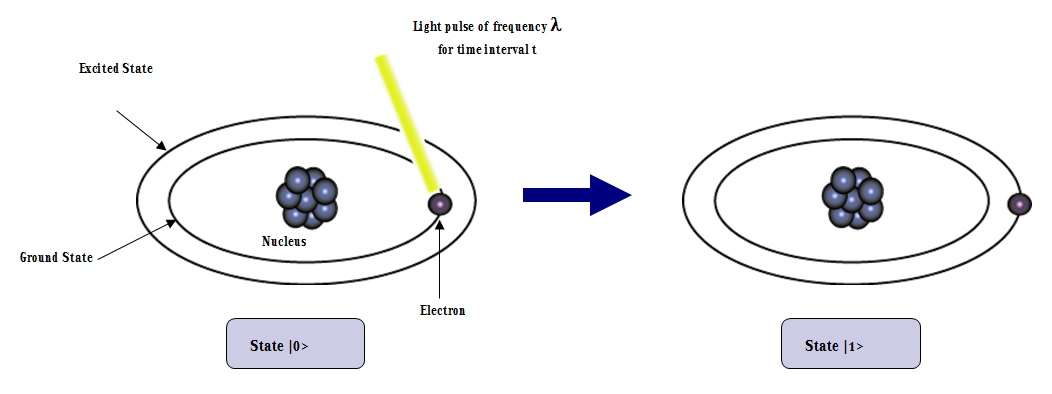
\includegraphics[scale=0.35]{img/qubitimplementation.jpeg}
       \caption[]{\label{img:qubitatom} A simple example of a physical qubit using the single valence electron of a hydrogen atom. Thereby, the electron's ground state can be defined as the \0 state of the qubit. By using a laser pulse, the electron can be excited into the next higher valence shell which can be defined as the qubit's \1 state. \textsuperscript{1}}
\end{figure}
\footnotetext[1]{Reprinted from RF Wireless World, n.d., Retrieved December 23, 2016, from \url{http://www.rfwireless-world.com/Terminology/Difference-between-Bit-and-Qubit.html}. Copyright 2012 by RF Wireless World.}

\pagebreak
A classical non-probabilistic bit can only take one of the two possible values at once. In contrast, qubits obey the laws of quantum mechanics, which gives rise to the important property that - besides being a definite \0 or \1 - they can also be in a superposition of the two states. Mathematically this is expressed as the linear combination of the states \0 and \1:
\begin{equation}
\label{equ: simplequbit}
\ket{\psi} = \alpha \ket{0} + \beta \ket{1}\, ,
\end{equation}
where $\alpha$ and $\beta$ are complex coefficients ($\alpha, \beta \in \mathbb{C}$) and are often referred to as amplitudes. Any amplitude $\eta$ can be further subdivided into a complex phase factor $e^{i\phi}$ and a non-negative real number $e$ such that
\begin{equation}
\label{equ: amplitude}
\eta = e^{i\phi}e\, .
\end{equation}
 
In Eq.~\ref{equ: simplequbit}, \0 is the Dirac notation for the qubit being in state 0 and can be represented as a two-dimensional vector in a complex two-dimensional vector space (called Hilbert space $\mathcal{H}_{2}$). First defined by \citeA{dirac1939new}, the object
\begin{equation}
\ket{\phi}\, ,
\end{equation}
is called a \emph{ket} and its Hermitian conjugate
\begin{equation}
\ket{\phi}^\dagger = \bra{\phi}\, ,
\end{equation}
is called a \emph{bra}. The Hermitian conjugate, denoted with a dagger ($\dagger$), of some e.g. two-dimensional column vector $c$ with complex entries $c_1$ and $c_2$:
\begin{equation}
c = \colvec{c_1\\c_2}\, ,
\end{equation}
is obtained by complex conjugating each entry and then transposing vector $c$:
\begin{equation}
c^\dagger = \colvec{c_1\\c_2}^\dagger = \begin{pmatrix}c_1^* & c_2^*\end{pmatrix}\, ,
\end{equation}
where complex conjugates are denoted with an asterisk ($*$). The Hermitian conjugate is defined for vectors as well as square matrices.

The inner product of a bra and a ket is called a \emph{bra-ket} and is written
\begin{equation}
\braket{\phi|\phi}
\end{equation}
Note that all later sections will make heavy use of this \emph{bra-ket notation}.

The quantum states \0 and \1 are called the computational basis states and they constitute an orthonormal basis of $\mathcal{H}_{2}$. When a qubit is expressed in terms of the two states \0 and \1 it is said to be in its \emph{standard basis}. For the sake of clarity, \0 and \1 can be represented as the 2-D vectors
\begin{equation}
\label{equ: 0and1kets}
\ket{0} \doteq  \colvec{1\\0} \quad \mathrm{and} \quad \ket{1} \doteq \colvec{0\\1} \, .
\end{equation}

Note that a ket and its vector representation are not the same object since a well-defined vector requires a basis whereas a ket does not demand specification of a basis. This thesis will make use of the $\doteq$ symbol when switching between the two different ways of representing a ket. Substituting the vectors from Eq.~\ref{equ: 0and1kets} into Eq.~\ref{equ: simplequbit} yields the vector representation of $\ket{\psi}$:
\begin{equation}
\label{equ: simplequbitvector}
\ket{\psi} \doteq \alpha \colvec{1\\0} + \beta \colvec{0\\1} = \colvec{\alpha\\\beta}\, .
\end{equation}

In the cases $\alpha = 1$ or $\beta = 1$ the qubit is not in a superposition but in the definite state \0 or \1 respectively. However, if for example $\alpha = \frac{1}{\sqrt{2}}$ and $\beta = \frac{i}{\sqrt{2}}$ the qubit is in a quantum superposition, impossible to achieve with a classical computer. This leads to another important qubit lifetime parameter - the \emph{transversal coherence} or \emph{phase damping time}. It is measured by preparing the equal superposition $\frac{\ket{0}+\ket{1}}{\sqrt{2}}$ and due to unavoidable interaction with the environment after some time $t$ the quantum behaviour will be lost, and the state will either be a definite \0 or \1 \cite{chuanglecturenotes}. The process of losing quantum behaviour is called \emph{decoherence}.

However, even though a qubit can be in a superposition of \0 and \1, when measured it will take the value \0 with a probability of
\begin{equation}
\label{equ:bornrule0}
\mathrm{Prob}(\ket{0}) = {|\alpha|}^{2}\, ,
\end{equation}
and \1 with a probability of 
\begin{equation}
\label{equ:bornrule1}
\mathrm{Prob}(\ket{1}) = {|\beta|}^{2}\, .
\end{equation}

The fact that the probability of measuring a particular state is equal the absolute value squared of the respective amplitude was first postulated by \cite{born1954statistical} and, thus, is called Born rule. Since the total probability of measuring any value has to be 1, the normalisation condition
\begin{equation}
\label{equ: normalization}
{|\alpha|}^{2} + {|\beta|}^{2} =  1\, ,
\end{equation}
must be satisfied. Therefore, a qubit is inherently probabilistic but when measured it collapses into a single classical bit (0 or 1). It follows that a measurement destroys information about the superposition of the qubit (the values of $\alpha$ and $\beta$). This constitutes one of the main difficulties when designing quantum algorithms since only limited information can be obtained about the final states of the qubits in the quantum computer.

Using spherical polar coordinates, a single qubit can be visualised on the so-called Bloch sphere by parameterising $\alpha$ and $\beta$ in Eq.~\ref{equ: simplequbit} as follows:
\begin{equation}
\label{equ: blochqubit}
\ket{\psi} = \cos\frac{\theta}{2} \ket{0} + e^{i \phi} \sin\frac{\theta}{2} \ket{1}\, .
\end{equation}
The Bloch sphere has a radius of 1 and is, therefore, a unit sphere. The \0 qubit state is defined to lie along the positive $\hat{z}$-axis and the \1 state is defined to lie along the negative $\hat{z}$-axis as labelled in Fig.~\ref{fig:blochsphere}. At this point, it is important to note that these two states are mutually orthogonal in $\mathcal{H}_{2}$ even though they are not orthogonal on the Bloch sphere. 

Qubit states on the Bloch equator such as the $\hat{x}$ and $\hat{y}$ coordinate axes represent equal superpositions where \0 and \1 both have measurement probabilities equal to $0.5$. The $\hat{x}$-axis for example represents the equal superposition $\ket{q} = \frac{1}{\sqrt{2}} \ket{0} + \frac{1}{\sqrt{2}} \ket{1}$. As illustrated in Fig.~\ref{fig:blochsphere} any arbitrary 2-D qubit state $\ket{\psi}$ can be decomposed into the polar angles $\theta$ and $\phi$ and visualised as a vector on the Bloch sphere. Such an object is called the Bloch vector of the qubit state $\ket{\psi}$. The Bloch sphere will be the main visualisation tool for qubit manipulations in this thesis.

\begin{figure}[!ht]
       \centering
       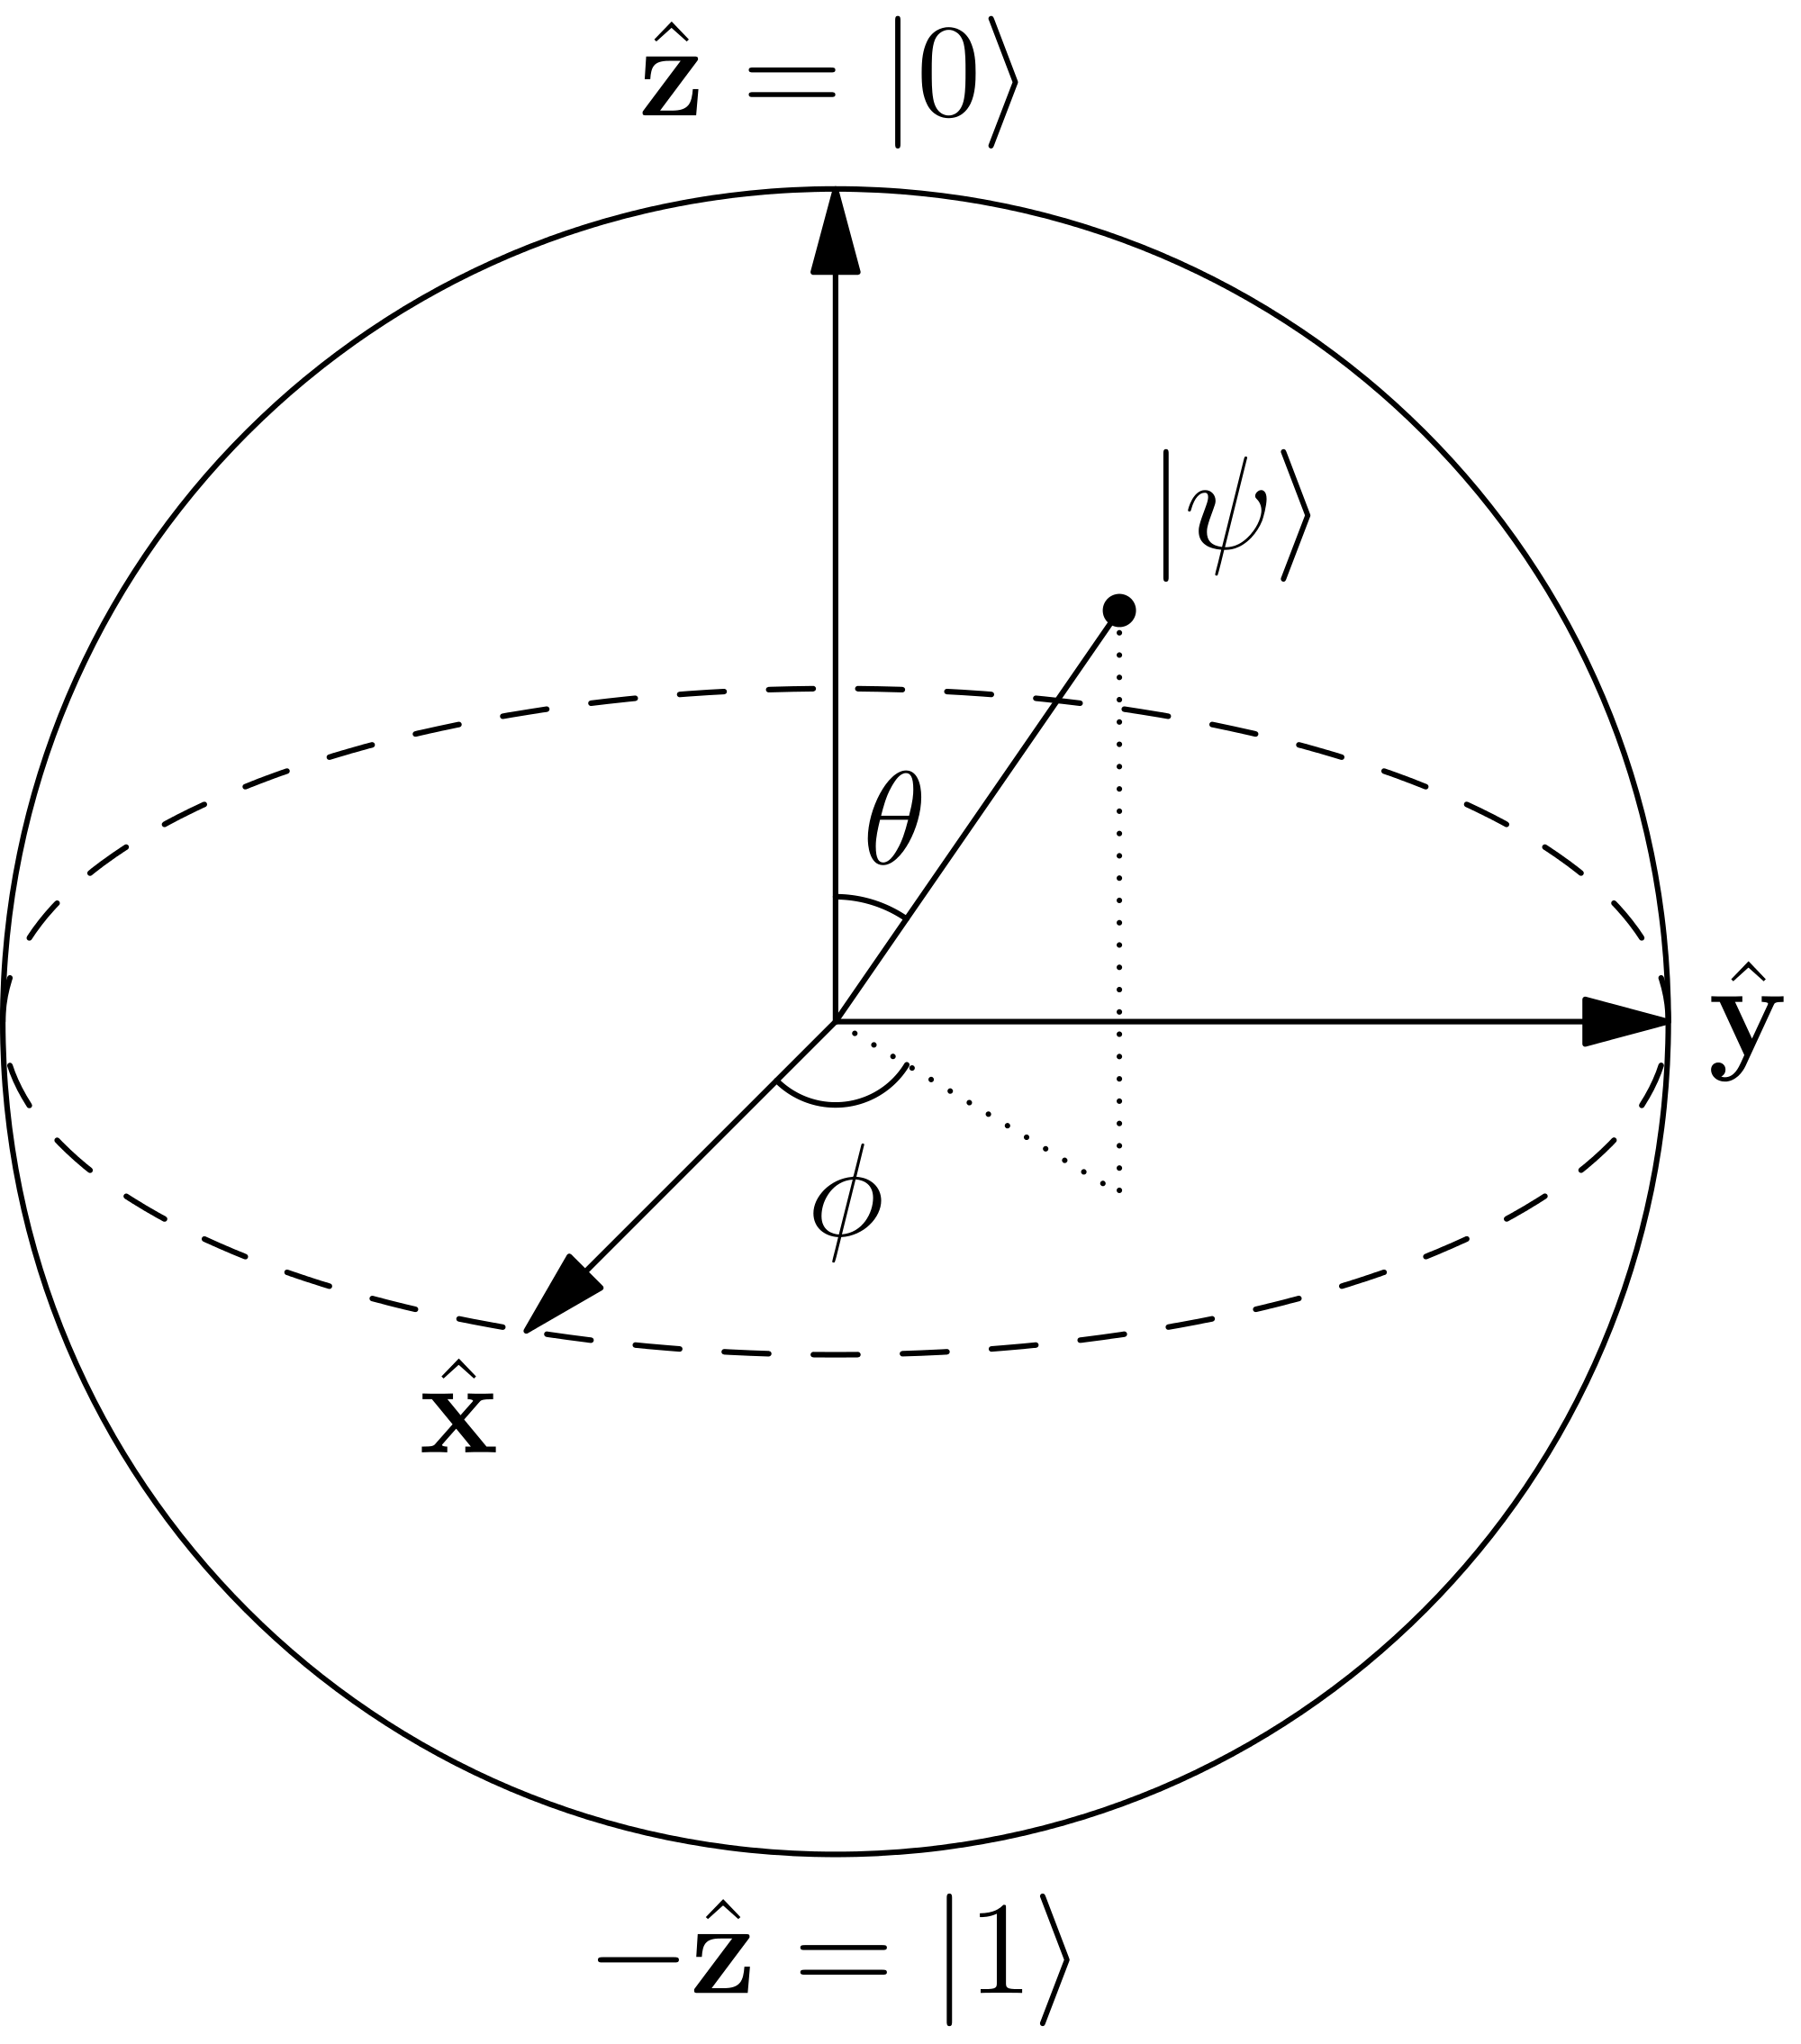
\includegraphics[scale=0.11]{img/blochsphere.png}
       \caption[]{\label{fig:blochsphere} An arbitrary single-qubit state $\ket{\psi} = \alpha \ket{0} + \beta \ket{1}$ can be visualised on the Bloch sphere by parameterising $\alpha = \cos\frac{\theta}{2}$ and $\beta = e^{i \phi} \sin\frac{\theta}{2}$ where $\theta$ is the polar and $\phi$ the azimuthal angle in spherical polar coordinates.\footnotemark[2]}
\end{figure}
\footnotetext[2]{Reprinted from Wikipedia, n.d., Retrieved September 7, 2016, from \url{https://en.wikipedia.org/wiki/Bloch_Sphere}. Copyright 2012 by Glosser.ca.}
\newpage

Similar to logic gates in a classical computer, a QC manipulates qubits, by means of quantum logic gates which will be introduced in detail in Section~\ref{subsec:quantumlogicgates}. Generally, an arbitrary quantum logic gate $U$ acting on a single qubit state is a unitary transformation which can be represented as a $2\times2$ matrix:
\begin{equation}
\label{equ:generalquantumgate}
U \doteq \begin{pmatrix}
 a & b \\ 
 c & d
 \end{pmatrix}\, ,
\end{equation}
whose action on $\ket{\psi}$ is defined as:
\begin{equation}
\label{equ:unitarytransformation}
U \ket{\psi} \doteq \begin{pmatrix}
 a & b \\ 
 c & d
 \end{pmatrix} \colvec{\alpha\\\beta} = \colvec{a\alpha+b\beta\\c\alpha+d\beta}\, .
\end{equation}

The matrix $U$ must be unitary which means that its determinant must equal unity:
\begin{equation}
\label{equ:unitarydef1}
\mid \mathrm{det}(U) \mid = 1\, ,
\end{equation}
and its Hermitian conjugate $U^\dagger$ must be equal to its inverse:
\begin{equation}
\label{equ:unitarydef2}
UU^\dagger = U^\dagger U = \mathbb{1} = UU^{-1} = U^{-1}U\, .
\end{equation} 

All quantum logic gates must be unitary since this preserves the normalisation of the qubit state it is acting on. The set of all two-dimensional complex unitary matrices with determinant one is called the special unitary group $\mathrm{SU}(2)$ and all single-qubit quantum gates are therefore elements of $\mathrm{SU}(2)$. Furthermore, a gate set $G$ consisting of $m$ quantum-gates $g_1,g_2,...,g_m$ is called a \emph{universal quantum gate set} when it is a dense subset of $\mathrm{SU}(2)$ as defined in the red box below.
\vspace{0.5cm}
\begin{redbox}
\textbf{Definition: Dense Subset of $\mathbf{SU(2)}$}\\
\newline
The gate set $G$ is a dense subset of $\mathrm{SU}(2)$ when given any quantum gate $W \in \mathrm{SU}(2)$ and any accuracy $\epsilon > 0$ there exists a product $J$ of gates from $G$ which is an $\epsilon$-approximation to $W$ \cite{dawson2005solovay}.
\end{redbox}
%\pagebreak
\subsection{Multi-qubit systems}
\label{subsec:multiqubitsystems}

A classical computer with one bit of memory is not particularly useful, and equally, a QC with one qubit is rather useless. To be able to perform large and complicated computations many individual qubits need to be combined to create a large QC. When moving from single to multi-qubit systems a new mathematical tool, the so-called tensor product (symbol $\otimes$), is needed. A tensor product of two qubits is written as
\begin{equation}
\label{equ:tensor}
\ket{\psi_1} \otimes \ket{\psi_2} = \ket{\psi_1}\ket{\psi_2} = \ket{\psi_1\psi_2}\, ,
\end{equation}
where the two last expressions omit the $\otimes$ symbol and are shorthand for a tensor product between two qubits.

A \emph{quantum register} of size $j$ is an alternative way of referring to a tensor product of $j$ qubits. For example, the state in Eq.~\ref{equ:tensor} is a quantum register consisting of two qubits. In QML algorithms, large quantum states are usually subdivided into several quantum registers fulfilling different purposes e.g. storing data or class labels. Consider, for example, a quantum state $\ket{\Phi}$ that is subdivided into two different quantum registers, a data ($d$) register with $n$ qubits and a class ($c$) register with two qubits. The state $\ket{\Phi}$ is then written
\begin{equation}
\label{equ:quantumregister}
\ket{\Phi} = \ket{d;c} = \ket{d_1,...,d_n;c_1,c_2}\, ,
\end{equation}
where semicolons are used to separate quantum registers.

In the vector representation a tensor product of two \0 kets (\textcolor{red}{red} and \textcolor{emerald}{green}) is defined as:
\begin{equation}
\label{equ:tensor2qubits}
\ket{\textcolor{red}{0}\textcolor{emerald}{0}} = \textcolor{red}{\ket{0}} \otimes \textcolor{emerald}{\ket{0}} \doteq \textcolor{red}{\colvec{1\\0}} \otimes \textcolor{emerald}{\colvec{1\\0}} = \colvec{\textcolor{red}{1}*\textcolor{emerald}{\colvec{1\\0}}\\\textcolor{red}{0}*\textcolor{emerald}{\colvec{1\\0}}} = \colvec{1\\0\\0\\0}\, .
\end{equation}

The last expression in Eq.~\ref{equ:tensor2qubits} shows that the two-qubit state $\ket{00}$ is no longer two but four-dimensional. Hence, it lives in a four-dimensional Hilbert space $\mathcal{H}_{4}$. A quantum gate acting on multiple qubits can therefore not have the same dimensions as a single-qubit gate (Eq.~\ref{equ:generalquantumgate}) which demands a new gate formalism for multi-qubit systems.

Consider aiming to apply an arbitrary single-qubit gate $U$ (Eq.~\ref{equ:generalquantumgate}) to the first qubit in the two-qubit state $\ket{00}$. The second qubit in the state $\ket{00}$ shall remain unchanged which, in other words, means applying the $2\times2$ identity matrix $\mathbb{1}$ to it. To perform these operations, one defines the tensor product of two single-qubit gates as
\begin{equation}
\label{equ:matrixtensorproduct}
\textcolor{red}{U} \otimes \textcolor{emerald}{\mathbb{1}} \doteq \textcolor{red}{\begin{pmatrix}
 a & b \\ 
 c & d
 \end{pmatrix}} \otimes \textcolor{emerald}{\begin{pmatrix}
 1 & 0 \\ 
 0 & 1
 \end{pmatrix}} = \begin{pmatrix}
 \textcolor{red}{a}*\textcolor{emerald}{\begin{pmatrix}
 1 & 0 \\ 
 0 & 1
 \end{pmatrix}} & \textcolor{red}{b}*\textcolor{emerald}{\begin{pmatrix}
 1 & 0 \\ 
 0 & 1
 \end{pmatrix}} \\ 
 \textcolor{red}{c}*\textcolor{emerald}{\begin{pmatrix}
 1 & 0 \\ 
 0 & 1
 \end{pmatrix}} & \textcolor{red}{d}*\textcolor{emerald}{\begin{pmatrix}
 1 & 0 \\ 
 0 & 1
 \end{pmatrix}}
 \end{pmatrix} = \begin{pmatrix}
 a & 0 & b & 0 \\ 
 0 & a & 0 & b \\ 
 c & 0 & d & 0 \\ 
 0 & c & 0 & d 
 \end{pmatrix}\, .
\end{equation}

Thus, the result of the tensor product $U \otimes \mathbb{1}$ can be represented as a unitary $4\times4$ matrix that can now be used to transform the $4\times1$ vector representing the $\ket{00}$ state in Eq.~\ref{equ:tensor2qubits}:
\begin{equation}
\label{equ:2qubitlineartransform1}
U \otimes \mathbb{1} \ket{00} \doteq \begin{pmatrix}
 a & 0 & b & 0 \\ 
 0 & a & 0 & b \\ 
 c & 0 & d & 0 \\ 
 0 & c & 0 & d 
 \end{pmatrix} \colvec{1\\0\\0\\0} = \colvec{a\\0\\c\\0}\, .
\end{equation}

One can also first perform the single qubit operations on the respective qubits, followed by the tensor product of the two resulting vectors:
\begin{equation}
\label{equ:2qubitlineartransform2}
(U \otimes \mathbb{1})(\ket{0} \otimes \ket{0})= U\ket{0} \otimes \mathbb{1}\ket{0} \doteq \begin{pmatrix}
 a & b \\ 
 c & d
 \end{pmatrix} \colvec{1\\0} \otimes \begin{pmatrix}
 1 & 0 \\ 
 0 & 1
 \end{pmatrix} \colvec{1\\0} = \colvec{a\\c} \otimes \colvec{1\\0} = \colvec{a\\0\\c\\0}\, .
\end{equation}

This formalism can be extended to any number of qubits, and the use of tensor products leads to an exponential increase in the dimensionality of the Hilbert space. Hence, $n$ qubits live in a $2^n$-dimensional Hilbert space ($\mathcal{H}_{2}^{\otimes n}$) and can store the content of $2^n$ classical bits. As an example, only 33 qubits can store the equivalent of $2^{33} = 8,589,934,592$ bits (= 1 gigabyte) which clearly bears the potential for enormous speedups in computations as will be demonstrated later.

When considering multi-qubit systems one will encounter quantum states that can or cannot be factorised. For example, consider reexpressing the last expression in Eq.~\ref{equ:2qubitlineartransform2} as
\begin{equation}
\label{equ:2qubitreexpressed}
\colvec{a\\0\\c\\0} = a\colvec{1\\0\\0\\0} + 0\colvec{0\\1\\0\\0} + c \colvec{0\\0\\1\\0} + 0\colvec{0\\0\\0\\1} \doteq  a\ket{00} + 0 \ket{01} + c \ket{10} + 0\ket{11}\, ,
\end{equation}
which can be factorised into the tensor product
\begin{equation}
\label{equ:2qubitfactorised}
a\ket{00} + c \ket{10} = (a\ket{0} + c \ket{1})\otimes \ket{0}\, .
\end{equation}

In contrast, consider one of the four famous Bell states:
\begin{equation}
\label{equ:2qubitnonfactorised}
\ket{\Psi^+} = \frac{\ket{01} + \ket{10}}{\sqrt{2}}\, .
\end{equation}
It is straightforward to verify that the two-qubit state $\ket{\Psi^+}$ cannot be factorised into a tensor product of two single-qubit states. Now imagine, that the two people Andile and Buhle are given two electrons prepared in the quantum state $\ket{\Psi^+}$. Andile keeps the first electron in the lab, and Buhle takes the second electron to her house. After some time $t$, Andile gets interested in measuring if his electron is in the $\ket{0}$ or $\ket{1}$ state and performs a measurement along the standard basis. By applying Born's rule to the quantum state $\ket{\Psi^+}$, Andile knows that he will measure his electron in either state \0 or \1 with equal probabilities of 0.5. Note that even though the exact state vector $\ket{\Psi^+}$ is known, the outcome of the measurement is still uncertain. By measuring his electron, he finds it to be in the $\ket{1}$ state. From Eq.~\ref{equ:2qubitnonfactorised} and knowing that measurement collapses a superposition, the post-measurement (PM) state $\ket{\Psi^+}_{PM}$ is
\begin{equation}
\label{equ:2qubitcollapsed}
\ket{\Psi^+}_{PM} = \ket{1_A0_B}\, ,
\end{equation}
where the subscripts indicate which electron belongs to Andile (A) and Buhle (B). Looking at this expression tells Andile that Buhle's electron must be in state $\ket{0}$ without having measured her electron! At her house, Buhle measures her electron one second after Andile has performed his measurement and indeed finds it to be in state $\ket{0}$. Note that the second electron was nowhere close to Andile and he was still able to determine its state by only measuring his electron. After repeating this experiment one thousand times, Andile and Buhle find perfect correlations in their results: whenever Andile measured his electron in state $\ket{0}$, Buhle found her electron in state $\ket{1}$ and vice versa.

Non-local correlations between qubit measurement outcomes is a peculiar quantum property of non-factorising quantum states and is called \emph{quantum entanglement}. It is an integral part of quantum computation and Section~\ref{subsubsubsec:cnotgate} will give a concrete example of how to create an entangled state in a QC.
%\pagebreak
\section{Quantum Logic Gates}
\label{subsec:quantumlogicgates}
Until this point, most introduced concepts came from the field of pure quantum theory. However, this section marks the important transition from quantum theory to the field of \emph{quantum information processing}. A classical computer processes information and performs computations by systematically manipulating bits through the application of logic gates e.g. NOT or XOR gates. Analogously, a quantum computer processes information and performs \emph{quantum computations} by manipulating qubits using \emph{quantum logic gates}, often just called \emph{quantum gates}. Usually, a sequence of such quantum gates is required to perform a certain task or solve a particular problem on a quantum computer. Such a sequence of quantum gates is called a \emph{quantum algorithm}. 

There are many different ways of realising a QC such as using trapped ions, photons or superconducting Josephson junctions, etc. \cite{clarke2008superconducting,haffner2008quantum,o2007optical}. Depending on the chosen substrate, different sets of quantum logic gates can be implemented and in order to run a quantum algorithm it has to be mapped to the available quantum hardware. Thus, quantum algorithms have to be translated (compiled) into a series of gates consisting only of quantum gates from the available universal gate set. This is referred to as \emph{quantum compiling}. 

The following subsections will introduce some major single and multi-qubit quantum logic gates that will be used extensively in the later sections of this thesis.
%In order to perform quantum computations, tools, analogous to the classical logic gates, are needed for qubit manipulation. 

\subsection{Single-qubit gates}
\label{subsubsec:singlequbitgates} 
%\subsubsection{Qubit flip (X) gate}
%\label{subsubsubsec:xgate}
%The quantum equivalent of the classical NOT logic gate is called X gate and is given by the 1\textsuperscript{st} Pauli matrix:
Quantum logic gates acting on single qubits can be represented as $2\times2$ unitary matrices (see Eq.~\ref{equ:generalquantumgate}) whose actions on a qubit can be visualised as rotations on the Bloch sphere. How a single-qubit quantum gate acts on a qubit, its properties and matrix representation will be illustrated using the example of the quantum equivalent of the classical NOT logic gate: the so-called X gate. The X gate can be represented by the $2\times2$ unitary matrix
\begin{equation}
X \doteq \begin{pmatrix}
 0 & 1 \\ 
 1 & 0
 \end{pmatrix}\, .
\end{equation}

The action of the X gate on the arbitrary qubit state $\ket{\psi}$ (Eq.~\ref{equ: simplequbitvector}) can be analysed using the gate's matrix and the qubit's vector representation. Applying some straightforward linear algebra yields
\begin{equation}
\label{equ:xverification1}
X \ket{\psi} = X (\alpha \ket{0} + \beta \ket{1}) \doteq \begin{pmatrix}
 0 & 1 \\ 
 1 & 0
 \end{pmatrix} \begin{pmatrix}
 \alpha  \\ 
 \beta
 \end{pmatrix} = \begin{pmatrix}
 \beta  \\ 
 \alpha
 \end{pmatrix} \doteq \beta \ket{0} + \alpha \ket{1}\, .
\end{equation}
Thus, applying the X gate to qubit state $\ket{\psi}$ swaps the amplitudes of the \0 and \1 states. More specifically, applying X to the \0 state results in the \1 state:
\begin{equation}
\label{equ:xverification2}
X \ket{0} \doteq \begin{pmatrix}
 0 & 1 \\ 
 1 & 0
 \end{pmatrix} \begin{pmatrix}
 1  \\ 
 0
 \end{pmatrix} = \begin{pmatrix}
 0  \\ 
 1 \end{pmatrix} \doteq  \ket{1}\, .
\end{equation}
In terms of the example with the valence electron of a hydrogen atom shown in Fig.~\ref{img:qubitatom} an X gate can be implemented by exciting the electron from the ground state $\ket{0}$ into the next higher electron valence shell, defined to be the $\ket{1}$ state, using a controlled laser pulse.
%consider the qubit initially being in state \0. Applying an X gate will flip the qubit into the \1 state which can be implemented in the lab by exciting the electron into the next highest electron valence shell using a controlled laser pulse.

The \0 state is recovered when applying X again to the \1 state:
\begin{equation}
\label{equ:xverification3}
X \ket{1} \doteq \begin{pmatrix}
 0 & 1 \\ 
 1 & 0
 \end{pmatrix} \begin{pmatrix}
 0  \\ 
 1
 \end{pmatrix} = \begin{pmatrix}
 1  \\ 
 0 \end{pmatrix} \doteq  \ket{0}\, .
\end{equation}

On the Bloch sphere, the X gate corresponds to an anti-clockwise $\pi$ rotation around the $\hat{x}$-axis as shown in Fig.~\ref{img:blochxgate}.

\begin{figure}[ht]
   \centering
   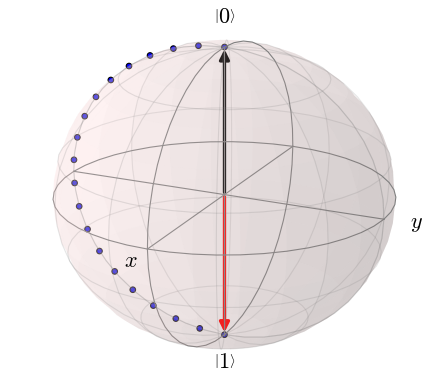
\includegraphics[width=0.75\textwidth]{img/blochxgate.png}
   \caption{Visualisation of the X gate action on the Bloch sphere. The figure shows the X gate transforming the \0 state (black $+\hat{z}$-axis) into the \1 state (red $-\hat{z}$-axis) by means of an anti-clockwise $\pi$ rotation around the $\hat{x}$-axis.}
   \label{img:blochxgate}
\end{figure}

From Eq.~\ref{equ:xverification1},~\ref{equ:xverification2} and~\ref{equ:xverification3} it follows that X is its own inverse as well as its own Hermitian conjugate:
\begin{align}
XX &= XX^\dagger = \mathbb{1}\, , \\
X &= X^{-1} = X^\dagger\, .
\end{align}

Based on the textbook by \citeA{nielsen2010quantum}, the action, circuit \& matrix representation and Bloch sphere visualisation for some of the most important single-qubit quantum logic gates are summarised in Table~\ref{tab:singlequbitgates}.

\begin{table}[H]
\caption{Table of some major single-qubit quantum logic gates.}\vspace{0.15em}
\label{tab:singlequbitgates}
\begin{tabular}{ C{0.3cm}  C{2cm}  C{1.5cm}  C{1.5cm} C{2.5cm} C{2cm} C{3.5cm}}\hline
Gate & Name & Circuit representation & Matrix & Description & Rotation & Bloch sphere \\ \midrule
$\mathbb{1}$ & Identity & 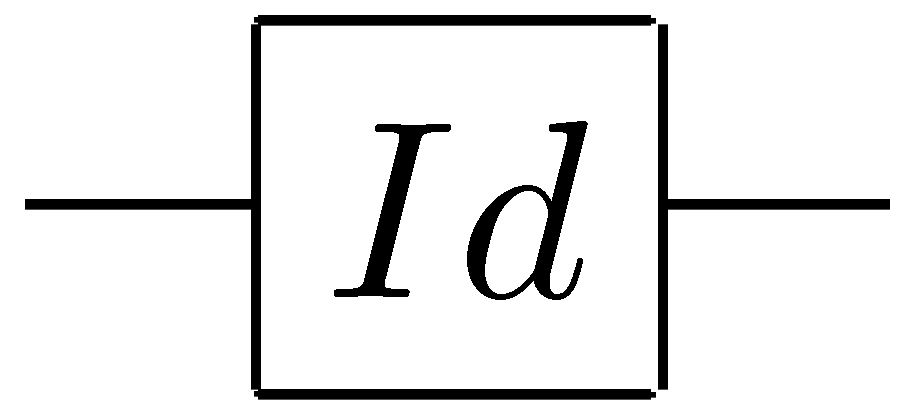
\includegraphics[width=0.1\textwidth]{img/identitycircuit.png} & $\begin{pmatrix}
 1 & 0 \\ 
 0 & 1
 \end{pmatrix}$ & Idle or waiting gate & - & - \\\midrule
X & Qubit flip & 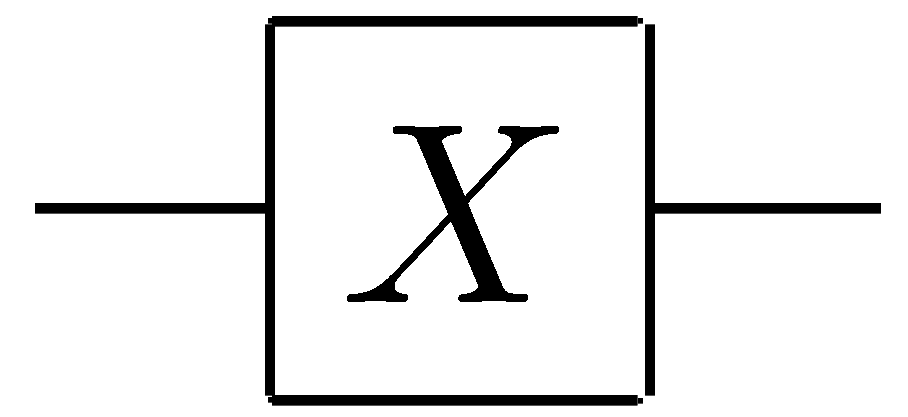
\includegraphics[width=0.1\textwidth]{img/xcircuit.png}  & $\begin{pmatrix}
 0 & 1 \\ 
 1 & 0
 \end{pmatrix}$ & Swaps amplitudes of \0 and \1 & $\pi$ rotation around $\hat{x}$ & 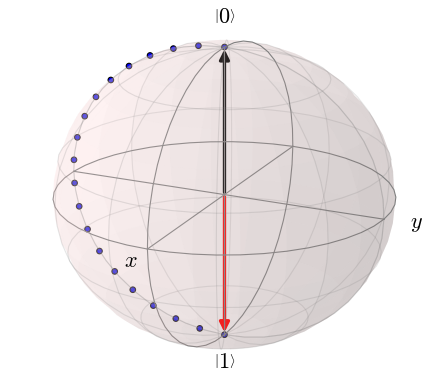
\includegraphics[width=0.2\textwidth]{img/blochxgate.png}\\\midrule
Y & Qubit \& phase flip & 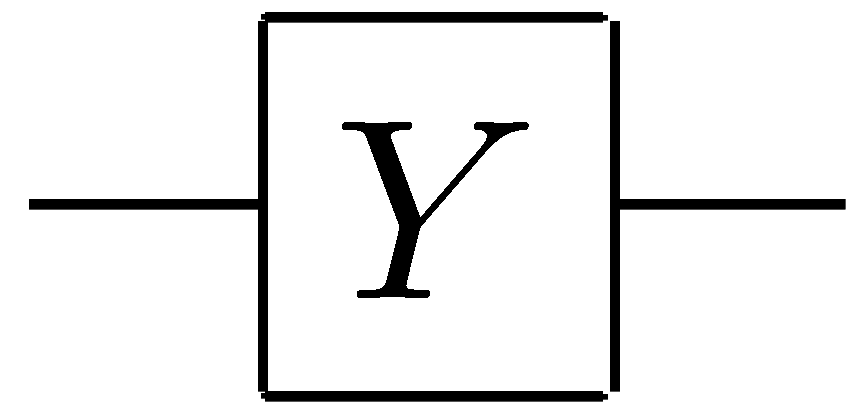
\includegraphics[width=0.1\textwidth]{img/ycircuit.png}  & $\begin{pmatrix}
 0 & -i \\ 
 i & 0
 \end{pmatrix}$ & Swaps amplitudes and introduces phase factor of $\pi$ (negative sign) to the \0 state & $\pi$ rotation around $\hat{y}$ &  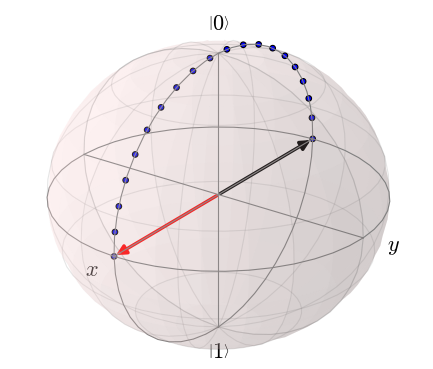
\includegraphics[width=0.2\textwidth]{img/blochygate.png}\\\midrule
Z & Phase flip & 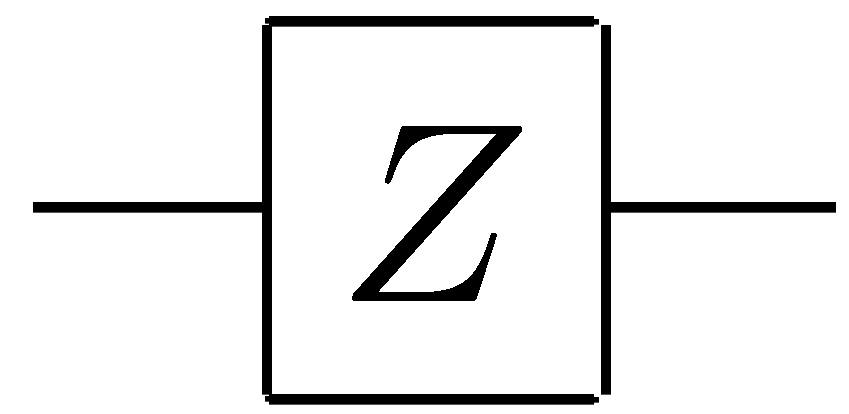
\includegraphics[width=0.1\textwidth]{img/zcircuit.png} & $\begin{pmatrix}
 1 & 0 \\ '
 0 & -1
 \end{pmatrix}$ & Introduces phase factor of $\pi$ (negative sign) to the \1 state & $\pi$ rotation around $\hat{z}$ & 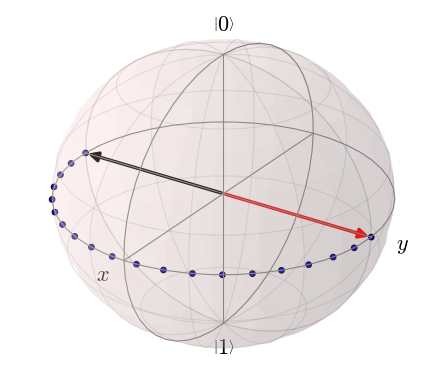
\includegraphics[width=0.2\textwidth]{img/blochzgate.png} \\\midrule 
H & Hadamard & 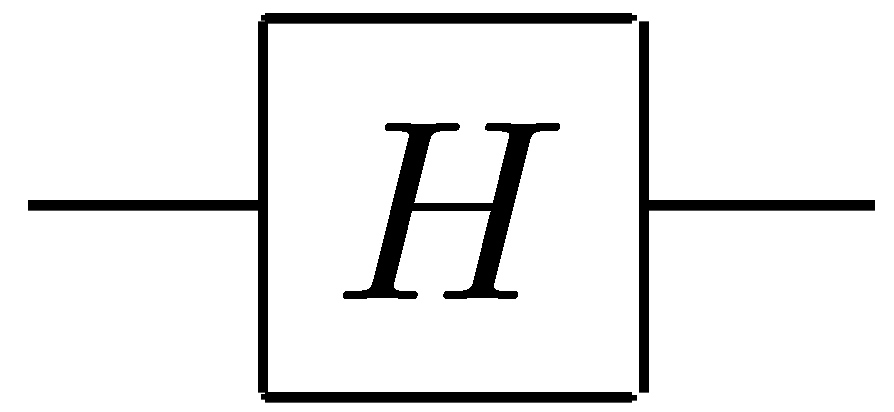
\includegraphics[width=0.1\textwidth]{img/hcircuit.png}  & $\begin{pmatrix}
 \frac{1}{\sqrt{2}} & \frac{1}{\sqrt{2}} \\ 
 \frac{1}{\sqrt{2}} & -\frac{1}{\sqrt{2}}
 \end{pmatrix}$ & Creates equal superposition & $\frac{\pi}{2}$ rotation around $\hat{y}$ and $\pi$ rotation around $\hat{x}$ & 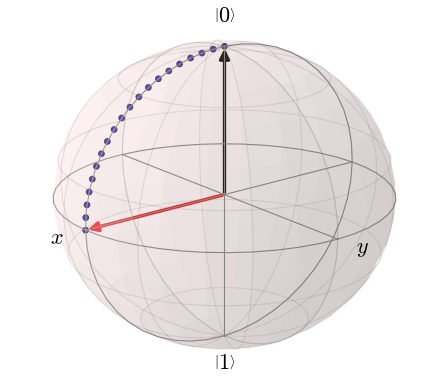
\includegraphics[width=0.2\textwidth]{img/blochhadamard.png}\\\midrule
S & $\frac{\pi}{2}$ rotation gate & 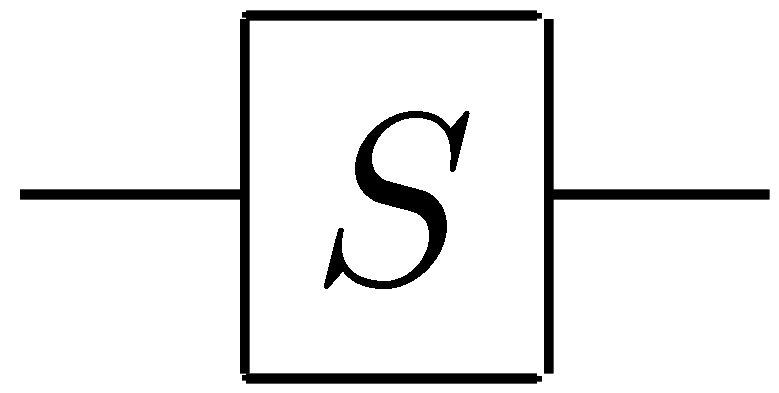
\includegraphics[width=0.1\textwidth]{img/scircuit.png} & $\begin{pmatrix}
 1 & 0 \\ 
 0 & i
 \end{pmatrix}$ & $\sqrt{Z}$ & $\frac{\pi}{2}$ rotation around $\hat{z}$ &  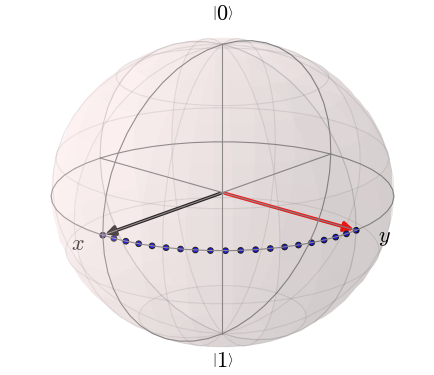
\includegraphics[width=0.2\textwidth]{img/blochsgate.png}\\\midrule
S$^\dagger$ & $-\frac{\pi}{2}$ rotation gate & 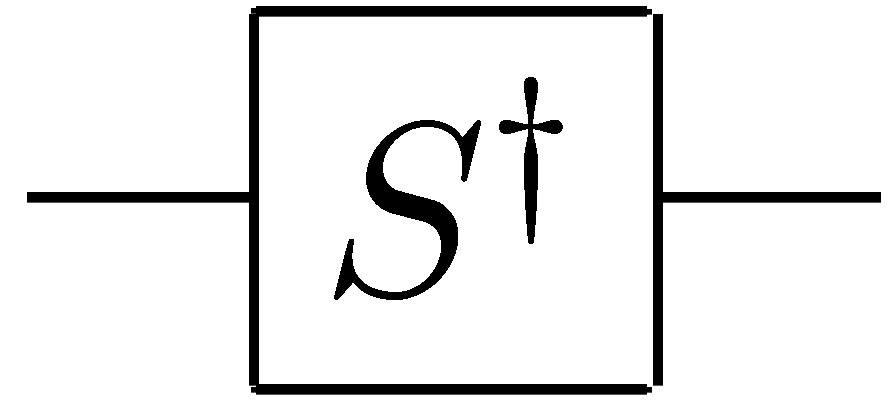
\includegraphics[width=0.1\textwidth]{img/sdcircuit.png} &  $\begin{pmatrix}
 1 & 0 \\ 
 0 & -i
 \end{pmatrix}$ & Hermitian conjugate of S & $-\frac{\pi}{2}$ rotation around $\hat{z}$ & \\\midrule
T & $\frac{\pi}{4}$ rotation gate & 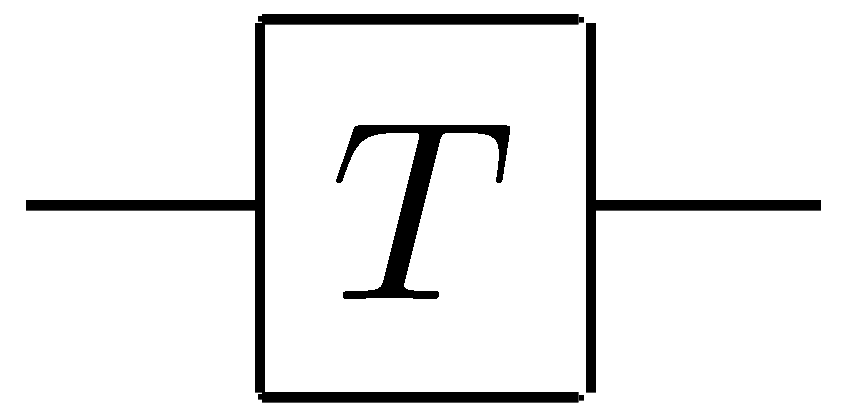
\includegraphics[width=0.1\textwidth]{img/tcircuit.png} & $\begin{pmatrix}
 1 & 0 \\ 
 0 & e^{\frac{i\pi}{4}}
 \end{pmatrix}$ & $\sqrt{S}$ & $\frac{\pi}{4}$ rotation around $\hat{z}$ & 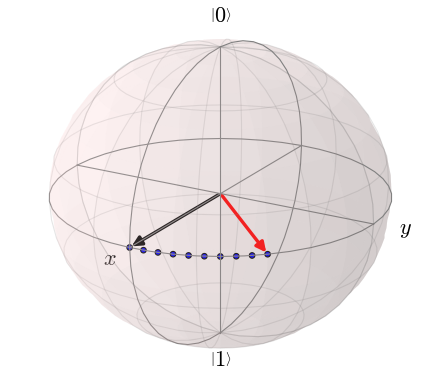
\includegraphics[width=0.2\textwidth]{img/blochtgate.png}\\\midrule
T$^\dagger$ & $-\frac{\pi}{4}$ rotation gate & 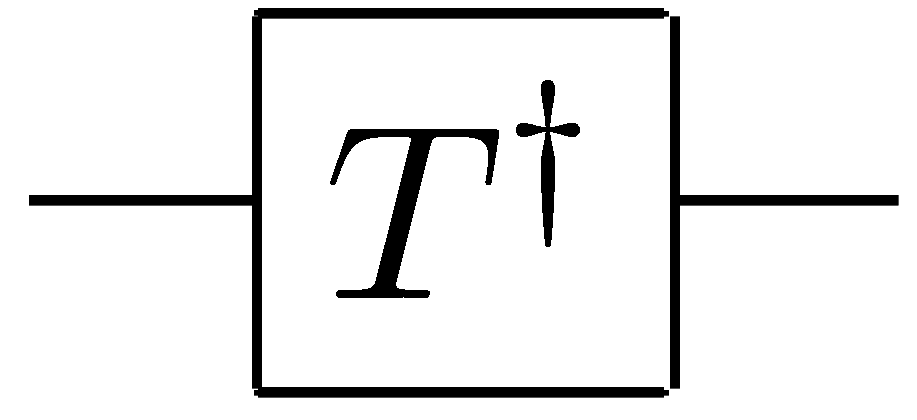
\includegraphics[width=0.1\textwidth]{img/tdcircuit.png} & $\begin{pmatrix}
 1 & 0 \\ 
 0 & e^{-\frac{i\pi}{4}}
 \end{pmatrix}$ & Hermitian conjugate of T & $-\frac{\pi}{4}$ rotation around $\hat{z}$ & \\\midrule
ZM & Z-basis measurement & 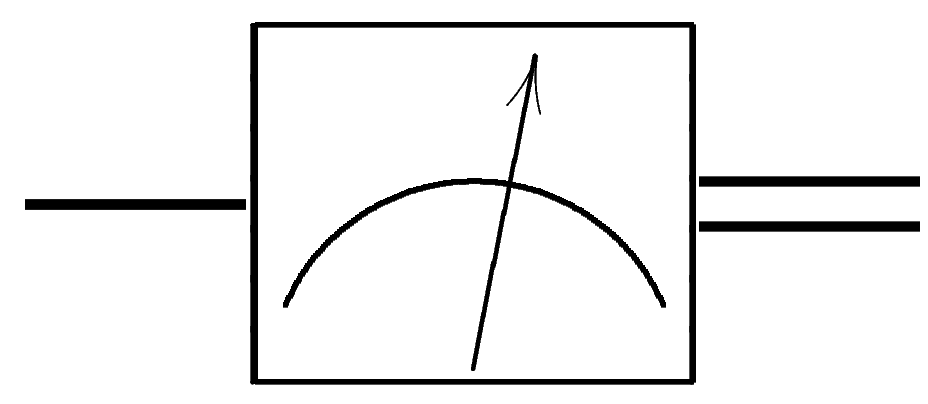
\includegraphics[width=0.1\textwidth]{img/measurecircuit.png} & - & Measurement in standard basis & Collapses the state & - \\
%\midrule
%BM & Bloch measurement & 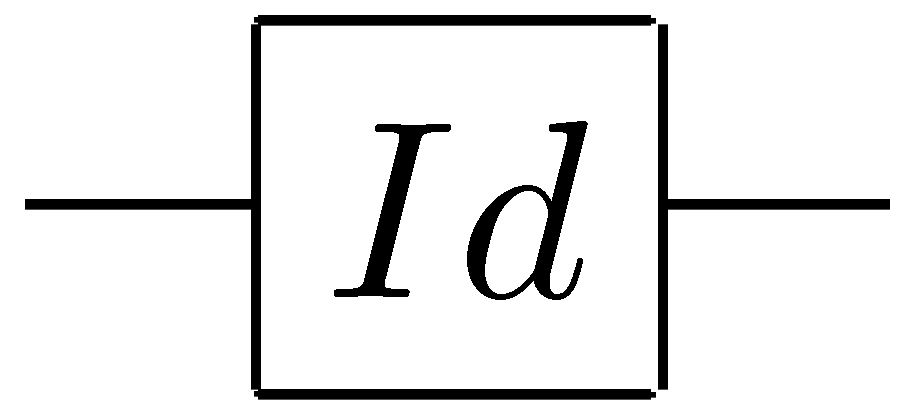
\includegraphics[width=0.1\textwidth]{img/identitycircuit.png} & - & Quantum state tomography & Collapses the state  & -\\
\end{tabular}
\end{table}


%%%%% SUBSECTION: MULTIPLE Q LOGIC GATES
\subsection{Multi-qubit gates}
\label{subsubsec:multiqubitgates}
\begin{table}[H]
\begin{center}
\begin{tabular}{l|lccc}\hline
Input & Output \\ \hline
00 & 00 \\
01 & 01 \\
10 & 11 \\
11 & 10 \\ \hline
\end{tabular}
\end{center}
\caption{Truth table for the CNOT quantum gate with the first qubit as control and the second qubit as target.}\vspace{1ex}
\label{tab:cnottruthtable}
\end{table}
%\subsubsection{Controlled-NOT gate}
%\label{subsubsubsec:cnotgate}
Multi-qubit quantum logic gates act on at least two qubits at the same time. Similar to single-qubit gates, an $n$-qubit quantum gate can be represented as a $2^n\times2^n$ unitary matrix. Since they involve multiple qubits, the Bloch sphere cannot longer be used to visualise their action. The two-qubit controlled NOT quantum gate will be used to demonstrate the properties, matrix representation and action of a two-qubit quantum gate. This can then easily be generalised to $n$-qubit quantum gates.

The controlled NOT or CNOT gate is given by the following $4\times4$ matrix:
\begin{equation}
\mathrm{CNOT} \doteq \begin{pmatrix}
 \mathbb{1} & 0 \\ 
 0 & X
 \end{pmatrix} = \begin{pmatrix}
 1 & 0 & 0 & 0 \\ 
 0 & 1 & 0 & 0 \\
 0 & 0 & 0 & 1 \\
 0 & 0 & 1 & 0 \\
 \end{pmatrix}\, .
\end{equation}

The CNOT gate takes two qubits, a control and a target qubit, as input. If and only if the control qubit is in the \1 state, the NOT (X) quantum gate is applied to the target qubit. In equations, the CNOT will always be followed by parentheses containing the control (c) qubit followed by the target (t) qubit: CNOT(c,t). The input-output relation, called truth table, for the CNOT gate is given in Table~\ref{tab:cnottruthtable} at the top of the page.

To demonstrate the usefulness of the CNOT gate consider starting with two unentangled qubits both in the \0 state,
\begin{equation}
\ket{\phi_0} = \ket{0} \otimes \ket{0} = \ket{00}\, .
\end{equation}
Applying the H gate onto the first qubit yields the following (still unentangled) state:
\begin{equation}
\ket{\phi_1} = (H \otimes \mathbb{1}) \ket{\phi_0} = (H \otimes \mathbb{1}) \ket{00} = \frac{1}{\sqrt{2}} \ket{00} + \frac{1}{\sqrt{2}} \ket{10}\, .
\end{equation}
Now consider applying the CNOT gate to the state $\ket{\phi_1}$ whereby the control qubit is coloured in \textcolor{red}{red} and the target qubit is coloured in \textcolor{emerald}{green}:

\begin{equation}
\label{equ:cnotexamples}
CNOT(\textcolor{red}{0},\textcolor{emerald}{1}) (\frac{1}{\sqrt{2}} \ket{\textcolor{red}{0}\textcolor{emerald}{0}} + \frac{1}{\sqrt{2}} \ket{\textcolor{red}{1}\textcolor{emerald}{0}}) = \frac{1}{\sqrt{2}} \ket{\textcolor{red}{0}\textcolor{emerald}{0}} + \frac{1}{\sqrt{2}} (\textcolor{red}{\mathbb{1}} \otimes \textcolor{emerald}{X}) \ket{\textcolor{red}{1}\textcolor{emerald}{0}} = \frac{1}{\sqrt{2}} \ket{\textcolor{red}{0}\textcolor{emerald}{0}} + \frac{1}{\sqrt{2}} \ket{\textcolor{red}{1}\textcolor{emerald}{1}}\, .
\end{equation}
The last expression in Eq.~\ref{equ:cnotexamples} is one of the famous Bell states which are a set of four maximally entangled quantum states. Another Bell state was used in the entanglement example in Section~\ref{subsec:multiqubitsystems}. Thus, this example demonstrates how the CNOT gate is crucial for the generation of entangled states since it applies the X gate to a target qubit depending on the state of a second control qubit.
%was used as an example (Eq.~\ref{equ:2qubitnonfactorised}) for entanglement in Section~\ref{subsec:multiqubitsystems} and it 

The three most important multi-qubit quantum gates CNOT, Toffoli and nCNOT are characterised in Table~\ref{tab:multiqubitgates}.

\begin{table}[H]
\caption{Table containing some major multi-qubit quantum logic gates where $c_j$ stands for the j\textsuperscript{th} control qubit and $\mathbb{1}_k$ for the kxk identity matrix.}\vspace{1em}
\label{tab:multiqubitgates}
\begin{tabular}{ c  C{1.8cm}  C{2cm}  c C{3cm}}\hline
Gate & Name & Circuit representation & Matrix & Description \\ \midrule
CNOT & Controlled NOT & 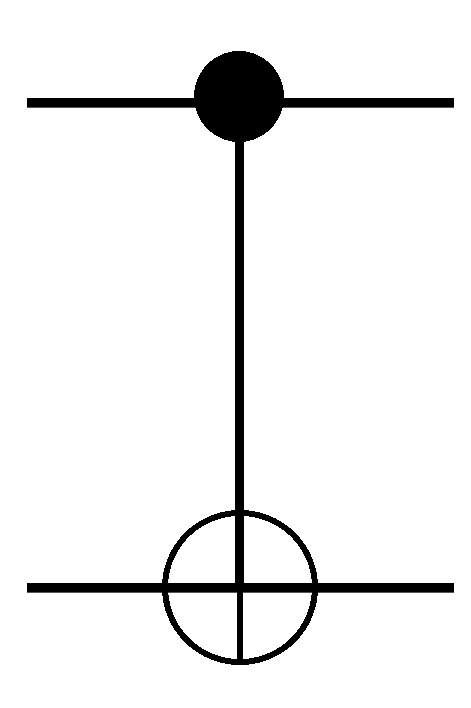
\includegraphics[width=0.1\textwidth]{img/cnotcircuit.png} & $\begin{pmatrix}
 \mathbb{1} & 0 \\ 
 0 & X
 \end{pmatrix} = \begin{pmatrix}
 1 & 0 & 0 & 0 \\ 
 0 & 1 & 0 & 0 \\
 0 & 0 & 0 & 1 \\
 0 & 0 & 1 & 0 \\
 \end{pmatrix}$ & CNOT($c_1$, target) \\\midrule
Toffoli & Controlled controlled NOT & 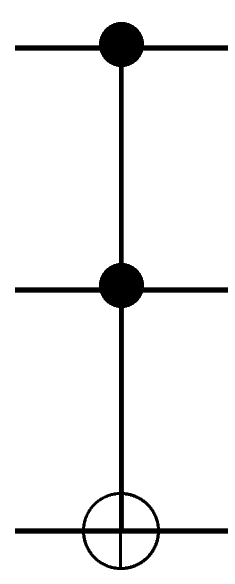
\includegraphics[width=0.1\textwidth]{img/ccnotcircuit.png}  & $\begin{pmatrix}
 \mathbb{1}_6 & 0 \\ 
 0 & X
 \end{pmatrix} = \begin{pmatrix}
 1 & 0 & 0 & 0 & 0 & 0 & 0 & 0 \\ 
 0 & 1 & 0 & 0 & 0 & 0 & 0 & 0 \\ 
 0 & 0 & 1 & 0 & 0 & 0 & 0 & 0 \\ 
 0 & 0 & 0 & 1 & 0 & 0 & 0 & 0 \\ 
 0 & 0 & 0 & 0 & 1 & 0 & 0 & 0 \\ 
 0 & 0 & 0 & 0 & 0 & 1 & 0 & 0 \\
 0 & 0 & 0 & 0 & 0 & 0 & 0 & 1 \\ 
 0 & 0 & 0 & 0 & 0 & 0 & 1 & 0 \\ 
 \end{pmatrix}$ & CCNOT($c_1$, $c_2$, target)\\\midrule
nCNOT & n-controlled NOT & -  & $\begin{pmatrix}
 \mathbb{1}_{2^n-2} & 0 \\ 
 0 & X
 \end{pmatrix}$ & nCNOT($c_1$,..,$c_n$, target) \\\midrule
\end{tabular}
\end{table}

%%%%% SECTION: MACHINE LEARNING

\section{Classical machine learning}
\label{subsec:classicalmachinelearning}

Machine learning (ML), a subfield of artificial intelligence, is aiming to enable computers to learn from data without a human explicitly programming its actions. It can be subdivided into the three major fields supervised \& unsupervised machine learning and reinforcement learning. The three areas can be most readily understood by considering the following three colloquial sentences:

\begin{redbox}
Supervised ML\\
- Based on \emph{input} and \emph{output} data\\
"I know how to classify this data, but I need an algorithm to do the computations for me."
\end{redbox}
\begin{greenbox}
Unsupervised ML\\
- Based on \emph{input} data only\\
"I have no clue how to classify this data, can the algorithm create a classifier for me?"
\end{greenbox}
\begin{bluebox}
Reinforcement learning\\
- Based on \emph{input} data only\\
"I have no clue how to classify this data, can the algorithm classify this data and I'll give it a reward if it's correct or I'll punish it if it's not."
\end{bluebox}

This thesis, specifically, is focusing on quantum-enhancements in the field of supervised machine learning only. The following section will introduce a well-known algorithm from the subfield of supervised ML: the $k$-nearest neighbour algorithm.

\subsection{Classical $k$-nearest neighbour algorithm}
\label{subsubsec:knearestneighbour}

Understanding the quantum version of the distance weighted $k$-nearest neighbour (kNN) algorithm as proposed by \citeA{Schuld2014} requires prior knowledge of the classical version of the algorithm that will be introduced in this subsection.

Imagine working for a search engine company and you are given the task of classifying unknown pictures of fruits as either apples or bananas. To train your classification algorithm, you are given five different pictures of apples and five different pictures of bananas. This will be called the \emph{training data set} ${D}_{T}$. The pictures in ${D}_{T}$ may be taken from various angles, in varying light settings and include different coloured apples and bananas. Two examples of such images are shown in Fig.~\ref{img:appleandbanana}. 

\begin{figure}[H]
  \begin{minipage}[t]{0.48\textwidth}
    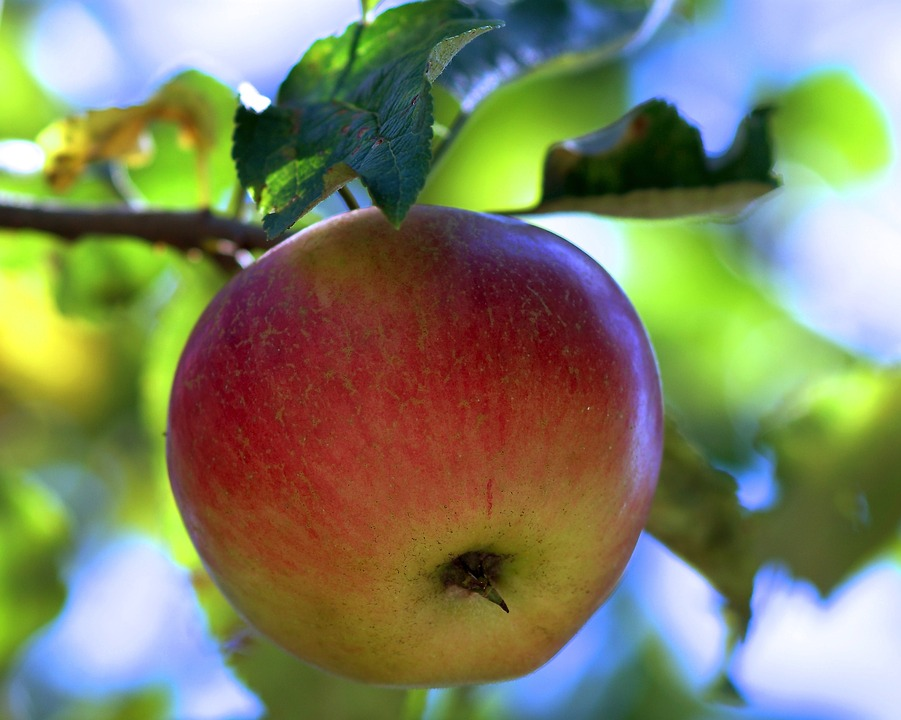
\includegraphics[width = \textwidth]{img/apple.jpg}
  \end{minipage}
  \hfill
  \begin{minipage}[t]{0.48\textwidth}
    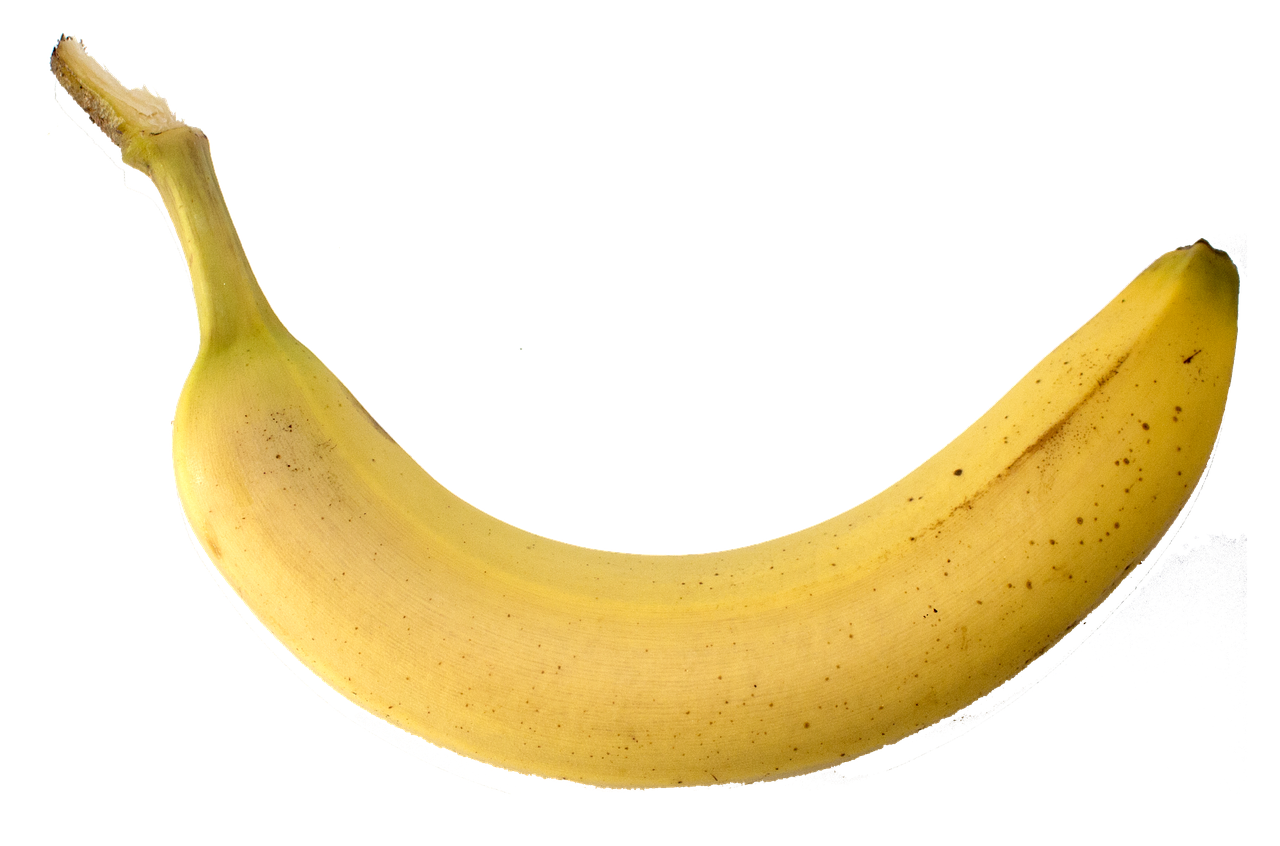
\includegraphics[width = \textwidth]{img/banana.png}
  \end{minipage}
  \caption[]{Pictures of apple and banana from training data set ${D}_{T}$.\footnotemark[3]}
  \label{img:appleandbanana}
\end{figure}

\footnotetext[3]{Reprinted from Pixabay, Retrieved December 24, 2016, from \url{https://pixabay.com/en/apple-red-fruit-frisch-vitamins-1632016/} and \url{https://pixabay.com/en/banana-fruit-yellow-1504956/}. Creative Commons Licence 2016 by Pixabay.}

Most of the time, using the full pixel representation of each picture for classification does not lead to optimal results. Therefore, the next step is to select a certain number of characteristic \emph{features} extracted from the pictures in the training set that can be used to differentiate apples from bananas. Such a feature might be the RGB value of the most frequent pixel colour since bananas and apples have different colour spectra. Using a measure of the curvature of the main object in the picture is another possibility since an apple is almost spherical whereas a banana looks more like a bend line.

By selecting and extracting features, the dimensionality of the training data set is drastically reduced from a few thousand pixels to a handful of features. The $m$ extracted features for the j\textsuperscript{th} picture are stored in the $m$-dimensional \emph{feature vector} $\vec{v}_{j}$. Mathematically, the training data set ${D}_{T}$ consists of ten feature vectors $\vec{v}_{0}, \vec{v}_{1},..,\vec{v}_{10}$ that are each assigned to either class $A$ (apple) or $B$ (banana). The training vectors are visualised as yellow and purple circles in Fig.~\ref{fig:knnconcept}.

Given a new picture of either a banana or an apple, you first extract the same $m$ features from it and store it in the input vector $\vec{x}$. From many algorithms, you decide to use the kNN algorithm since it is a non-parametric classifier meaning it makes no prior assumption about the class of the new picture. Given a new unclassified input vector $\vec{x}$ (red star in Fig.~\ref{fig:knnconcept}), the algorithm considers the $k$ nearest neighbours within the training set (using a predefined measure of distance) and classifies $\vec{x}$, based on a majority vote, as either $A$ or $B$. Thereby, $k$ is a positive integer, usually chosen to be small and its value determines the classification outcome. Namely, in the case $k = 3$ in Fig.~\ref{fig:knnconcept}, vector $\vec{x}$ will be classified as class B (purple) but in the case $k = 6$ it will be labelled class A (yellow).

\begin{figure}[H]
      \centering
       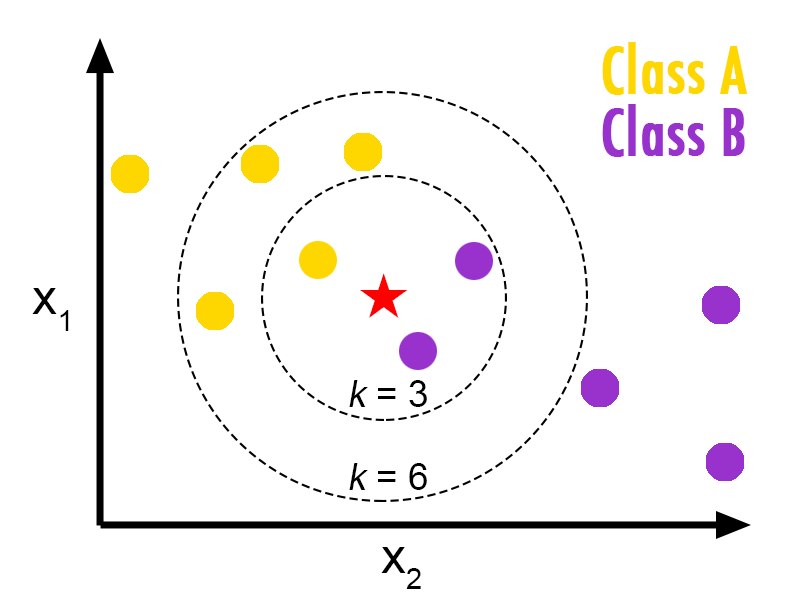
\includegraphics[scale=0.8]{img/knn-concept.png}
       \caption[]{\label{fig:knnconcept} Visualisation of a kNN classifier\footnotemark[4]}
\end{figure}

\footnotetext[4]{Reprinted from GitHub, Burton de Wilde, Retrieved September 13, 2016, from \url{http://bdewilde.github.io/blog/blogger/2012/10/26/classification-of-hand-written-digits-3/}. Copyright 2012 by Burton de Wilde.}

In the case of $k = 10$, $\vec{x}$ would simply be assigned to the class with the most members. In this case, the training vectors should be given distance-dependent weights (such as $\frac{1}{distance}$) to increase the influence of closer vectors over more distant ones.

\subsection{Algorithmic time complexity: Big-O notation}
\label{subsubsec:algcomplexity}

%\subsubsection{Big-O notation}
%\label{subsubsubsec:bigO}
In the fields of computer science and quantum information, the so-called \emph{Big-O notation}, first described by \citeA{bachmann1894analytische}, is often used to describe how the runtime of an algorithm depends on variables such as the desired accuracy, the number of input vectors or their size. Hence, this is a way of quantifying the \emph{algorithmic time complexity} of a quantum algorithm. In the later sections of this thesis, the Big-O notation will be used as a tool to quantify possible quantum speedups in kNN quantum machine learning algorithms.

\begin{redbox}
\textbf{Definition: Big-O $\mathcal{O}$}\\
\newline
For any monotonic functions $t(n)$ and $g(n)$ defined on a subset of the real numbers (${\rm I\!R}$), one says that $t(n) = \mathcal{O}(g(n))$ if and only if when there exists constants $c \geq 0$ and $n_0 \geq 0$ such that

\begin{equation}
\mid t(n) \mid \quad \leq \quad c\text{ }\mid g(n) \mid\, , \quad \text{for all } n \geq n_0\, .
\end{equation}
\end{redbox}
\begin{redbox}
\begin{figure}[H]
      \centering
       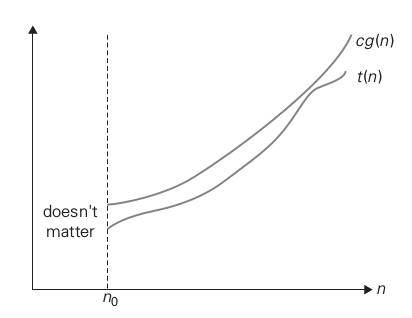
\includegraphics[scale=0.3]{img/asymptoticupperbound.png}
       \caption[]{\label{fig:upperasym} Visualisation of $c\text{ }g(n)$ being an upper asymptotic bound for the function $t(n)$\footnotemark[5]}
\end{figure}

\footnotetext[5]{Reprinted from Anany Levitin and Soumen Mukherjee. Introduction to the Design \& Analysis of Algorithms. Reading, MA: Addison-Wesley, 2003. Copyright 2012 by Levitin \& Mukherjee.}

This implies that the function $t(n)$ does not grow at a faster rate than $g(n)$, or in other words that some constant multiple of the function $g(n)$ is an upper asymptotic bound for the function $t(n)$, for all $n\rightarrow \infty$.
\end{redbox}

Fig.~\ref{fig:algcomplexities} provides a good visual comparison between common algorithmic complexity classes regarding their relation to the input size $n$. It can be seen that the best possible algorithmic time complexity is constant time, $\mathcal{O}(1)$, that is being independent of the size of the input data e.g. determining if a binary number is even or odd. An algorithm is still considered excellent if it runs in logarithmic time $\mathcal{O}(log(n))$. Linear search algorithms, for example, are linear in time expressed as $\mathcal{O}(n)$. More complex sort algorithms like "bubble sort" have a higher time complexity and often run in quadratic time ($\mathcal{O}(n^2)$). Furthermore, algorithms with complexity $\mathcal{O}(n^c)$ are said to run in polynomial time for some $c > 2$. If an algorithm has time complexity $\mathcal{O}((log(n))^c)$ for some $c \geq 1$ it is called polylogarithmic. The highest complexity classes are exponential $\mathcal{O}(c^n)$ with $c \geq 1$ and factorial time $\mathcal{O}(n!)$. 
%For example, solving the travelling salesman problem using brute-force search runs in factorial time.

\begin{figure}[H]
      \centering
       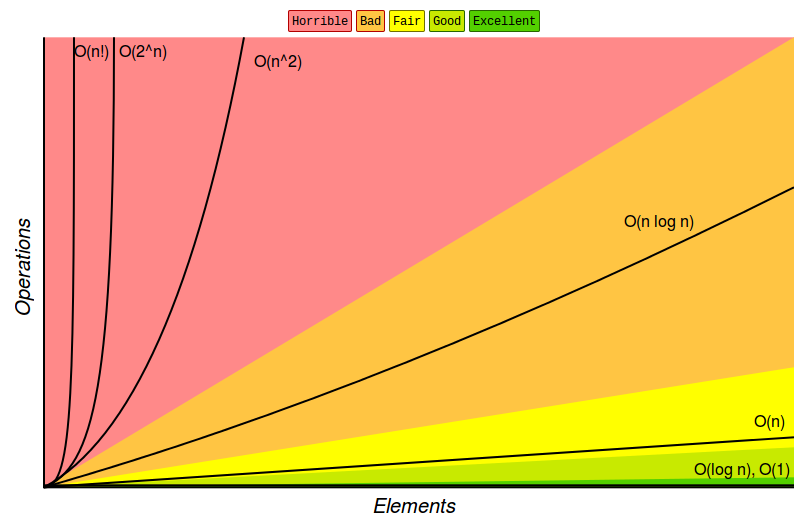
\includegraphics[scale=0.35]{img/bigocomplexity.png}
       \caption[]{\label{fig:algcomplexities} Overview of some major algorithmic complexity classes. In the figure, the number of operations (vertical axis) is plotted against the number of elements $n$ in the input data vector (horizontal axis). Based on colour coding defined on top of the table the following algorithmic time complexity classes are illustrated: constant time $\mathcal{O}(1)$, logarithmic time $\mathcal{O}(log(n))$, linear time $\mathcal{O}(n)$, linearithmic time $\mathcal{O}(n log(n))$, quadratic time $\mathcal{O}(n^2)$, exponential time $\mathcal{O}(2^n)$ and factorial time $\mathcal{O}(n!)$.\footnotemark[6]}
\end{figure}
\footnotetext[6]{Reprinted from Big-O Cheatsheet, Retrieved December 28, 2016, from \url{http://bigocheatsheet.com/}. Copyright 2016 by Big-O Cheatsheet.}

%TRANSITION TO NEXT SECTION NEEDED!

\chapter{Methods}\label{sec:methods}

The entirety of the research for this thesis is performed with pen and paper and a computer running the Linux operating system Ubuntu. The programming language Python, with its very intuitive syntax and extensive libraries for scientific computing and plotting, was used for the calculations and most of the plots for this thesis. More specifically, the open-source QuTiP library\footnotemark[7] for Python was used to create the Bloch sphere plots. All function plots were embedded directly into \LaTeX  by using the pgfplots package\footnotemark[8].

\footnotetext[7]{The open-source QuTiP library for Python may be downloaded from \url{http://qutip.org/}.}
\footnotetext[8]{The \LaTeX  pgfplots package may be downloaded from \url{https://www.ctan.org/pkg/pgfplots}.}

For the implementation of the quantum kNN algorithm, there are two fundamentally different ways: Running it a) by simulating a QC or b) by actually executing it on a real QC. The required tools for both possibilities will be explained in the following subsections.

\section{Liqui$\ket{}$}
\label{subsec:simulation}

Classical computers can be used to simulate the behaviour of small quantum computers. As outlined in Section~\ref{subsec:multiqubitsystems}, a QC with $n$ qubits can store the equivalent of $2^n$ classical bits in its $2^n$ amplitudes. It follows, that using a classical computer to simulate a QC with $n$ qubits requires storing all the $2^n$ amplitude values. Each amplitude has a complex and real part, hence, requiring two floating-point numbers to be stored. A floating-point number is encoded into 32 bits and storing each amplitude, thus, requires at least 64 classical bits of memory \cite{lambropoulos2007fundamentals}. As a result, a classical computer with at least $2^n\cdot64$ classical bits of random-access memory (RAM) is required to simulate an $n$-qubit quantum computer. As an example, only around two gigabytes (GB) of classical RAM are needed to simulate 25 qubits. Yet, the simulation of a QC with 44 qubits would require the world's fastest supercomputer Sunway TaihuLight with more than one petabyte of classical RAM \cite{chinasupercomputer}. Thus, simulating a quantum computer is associated with exponential computational costs thereby limiting the number of simulated qubits. Although, since current state-of-the-art quantum technology uses around ten qubits, a classical computer can still be used for simulation.

For the quantum computing simulations in this thesis the quantum simulation toolsuite Liqui$\ket{}$ developed by \citeA{liquid} will be used. Liqui$\ket{}$ is based on the functional programming language F\# and allows for simulation of up to 30 qubits \cite{microsoftresearch}. It comes with a large palette of predefined single and multi-qubit quantum logic gates and allows for custom-defined quantum gates such as nCNOT and rotation gates controlled by $n$ qubits which are crucial for some of the work done in this thesis. A short piece of example code from Liqui$\ket{}$ written in F\# is shown in Fig.~\ref{fig:liquidsnippet}. For all quantum simulations in this thesis, a Lenovo ThinkPad T450 with an Intel i5 processor (2 cores) and 8GB RAM is used.

\begin{figure}[H]
      \centering
       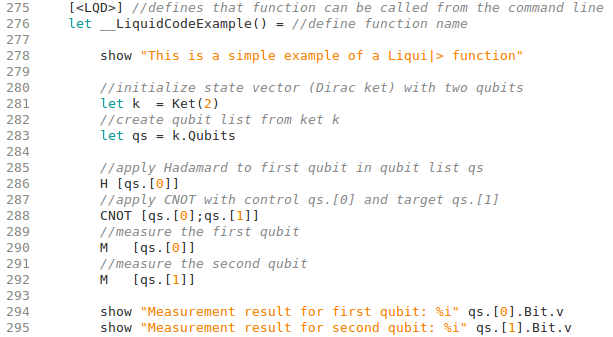
\includegraphics[scale=0.6]{img/liquidcodesnippet.png}
       \caption{\label{fig:liquidsnippet} F\# code snippet from Microsoft's quantum simulation toolsuite Liqui$\ket{}$. First, the code initialises two qubits in state $\ket{00}$ and applies an H gate to the first qubit leading to the state $\frac{\ket{00}+\ket{10}}{\sqrt{2}}$. Next, a CNOT gate, using the first and second qubit as control and target respectively, is applied. This leads to the maximally entangled state $\frac{\ket{00}+\ket{11}}{\sqrt{2}}$. Subsequently, both qubits are measured and the resulting bit values are displayed in the console.}
\end{figure}

\section{IBM Quantum Experience}
\label{subsec:ibmqc}

Since May 2016, IBM has enabled public cloud access to their experimental quantum processor containing five non-error-corrected superconducting qubits located at the IBM Quantum Lab at the Thomas J Watson Research Center in Yorktown Heights, New York \cite{ibmquantumcomputer}. Instead of only simulating on classical hardware, this opens up the possibility of executing the QML kNN algorithm on actual quantum hardware.

The so-called IBM Quantum Experience\footnotemark[9] provides the user with access to their \emph{quantum composer} which is the main tool for algorithm design. The quantum composer shown in Fig.~\ref{fig:composer} consists of 5 horizontal lines, one for each qubit, and enables the user to choose from a universal gate set (bottom of Fig.~\ref{fig:composer}) consisting of the following 10 quantum logic gates: $\mathbb{1}$, X, Y, Z, H, S, S$^\dagger$, T, T$^\dagger$ and CNOT. Additionally, there are two different types of measurement:
\begin{enumerate}[(a)]
\item A measurement in the standard basis, resulting in a probability distribution over the \0 and \1 state.
\item A Bloch measurement that visually projects the state onto the Bloch sphere. This is achieved by performing so-called \emph{quantum state tomography}\footnotemark[10] on the qubit while ignoring possible entanglement with other qubits \cite{ibmqetomo}.
\end{enumerate}
Through simple drag and drop the user can move any of those quantum logic and measurement gates into the quantum composer to create a quantum algorithm. However, the current version of the IBM Quantum Experience only allows the application of up to 40 quantum logic and measurement gates per qubit in the composer.
\footnotetext[9]{The IBM Quantum Experience can be accessed via \url{https://quantumexperience.ng.bluemix.net/qstage/}.}
\footnotetext[10]{A detailed explanation of quantum state tomography exceeds the scope of this thesis. The interested reader is referred to \citeA{altepeter649quantum}.}

\begin{figure}[H]
      \centering
       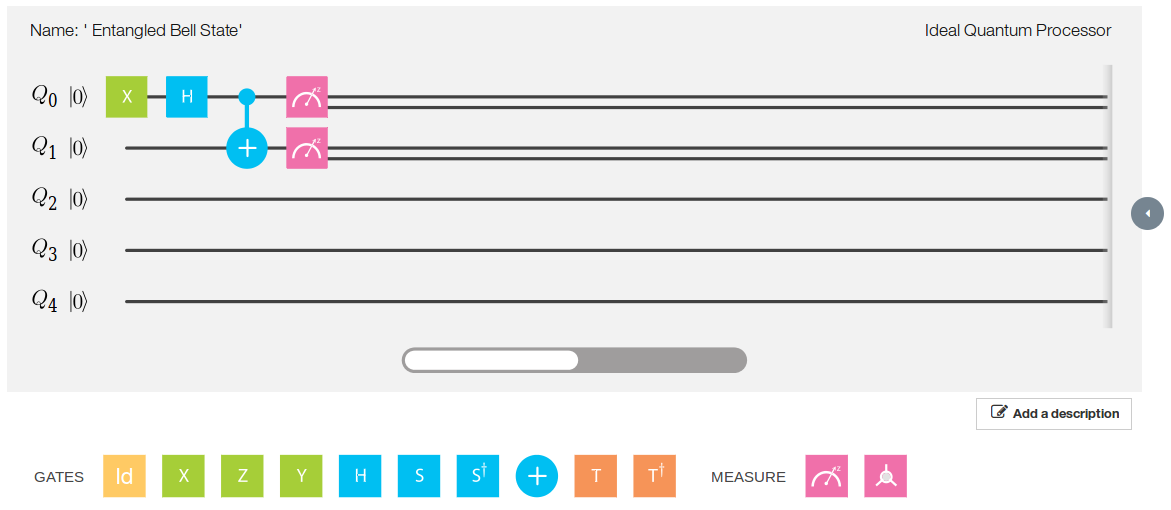
\includegraphics[scale=0.36]{img/ibmcomposer.png}
       \caption[]{\label{fig:composer} Screenshot showing the IBM Quantum Composer. For each of the five qubits $Q_0$,...,$Q_4$ there is a horizontal line with 40 available quantum gate slots. Quantum gates chosen from the universal gate set at the bottom can be dragged and dropped into the quantum composer to create a quantum algorithm.\footnotemark[11]}
\end{figure}
\footnotetext[11]{Screenshot was taken from \url{https://quantumexperience.ng.bluemix.net/qstage/#/editor}.}

After registration, each user receives a limited number of units that are required to execute algorithms on the real quantum processor. A minimum of three units is required to send the gate sequence of a composed algorithm to IBM's QC in New York. Then, depending on the waiting queue and the availability of the QC the results will be send back via email within a few minutes or days. The IBM Quantum Experience also allows for free quantum simulations under ideal or real conditions which provide a great tool for experimentation without spending user units.

The main limitation of the IBM Quantum Experience are the qubit decoherence times since they restrict the maximum number of possible operations before the qubits lose their quantum behaviour and their quantum information. Therefore, the number of quantum gates per qubit is currently limited to only 40 which essentially means 39 logic gates and one measurement gate. According to the qubit calibration results shown in Fig.~\ref{fig:calibration}, the amplitude damping times of the five qubits range from \SI{52.3}{\micro\second} to \SI{81.5}{\micro\second}. Furthermore, the phase damping times range from \SI{60.9}{\micro\second} to \SI{112.4}{\micro\second}. Currently, the implementation of a single qubit quantum logic gate takes 130ns and applying a CNOT gate takes 500ns \cite{ibmgatetimes}.

\begin{figure}[H]
      \centering
       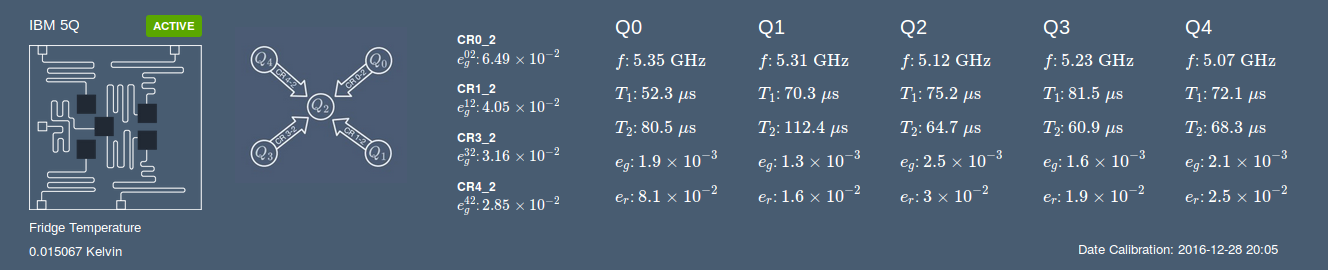
\includegraphics[scale=0.33]{img/ibmcalibration.png}
       \caption[]{\label{fig:calibration} Screenshot of IBM quantum processor calibration results showing the chip architecture, qubit arrangements, decoherence times and qubit error rates (28. December 2016 - 20:05).\footnotemark[12]}
\end{figure}
\footnotetext[12]{Screenshot was taken from \url{https://quantumexperience.ng.bluemix.net/qstage/#/editor}.}

\chapter{Literature Review: Quantum-enhanced Machine Learning}\label{sec:qml}

Classical machine learning takes classical data as input and learns from it using classical algorithms executed on classical computers: \citeA{aimeur2006machine} refer to this as C/C (classical data with classical algorithm). One enters the field of quantum machine learning when either \emph{quantum data} or quantum algorithms are combined with ideas from classical machine learning. Thus, \citeA{aimeur2006machine} divide the field of quantum machine learning into three different subfields: 1) C/Q - classical data with quantum algorithm, 2) Q/C - quantum data with classical algorithm and 3) Q/Q - quantum data with quantum algorithm. Thereby, quantum data includes any data describing a quantum mechanical system such as e.g. the Hamiltonian or state vector of a quantum system.

The subfield Q/C processes quantum data with classical machine learning algorithms. For example, \citeA{carrasquilla2016machine} used Google's deep learning library TensorFlow to identify the current phase of and phase transitions in quantum systems. Subfield Q/Q  is the union of C/Q and Q/C and deals with the processing of quantum data using quantum algorithms e.g. learning the Hamiltonian of a quantum system using quantum machine learning algorithms.

The topic of this thesis is embedded within the subfield C/Q that aims to develop quantum algorithms for machine learning tasks involving classical data. This subfield is also called \emph{quantum-enhanced machine learning} since smart algorithm design can harness quantum parallelism and quantum interference to speed up classical machine learning algorithms. The following sections will introduce some main concepts from the field of quantum-enhanced machine learning. More specifically, Section~\ref{subsec:quantumknearestneighbour} presents the quantum version of the classical $k$-nearest neighbour algorithm whose quantum simulation will be discussed extensively in Section~\ref{subsec:qubitKNNresults}. However, since a quantum algorithm is a sequence of quantum gates, it can only manipulate quantum and not classical bits. Therefore, the next section will first outline how classical data can be transferred into quantum states that can then be used for quantum computations.

%WRITE ANOTHER PARAGRAPH HERE!

\newpage
\section{Quantum state preparation}
\label{subsec:quantumstatepreparation}

\emph{Quantum state preparation} is the process of preparing a quantum state that accurately represents a vector containing classical (normalised) data. In order to apply any quantum machine learning algorithm to classical data, quantum state preparation always needs to be performed first. Therefore, the reader needs to be familiar with the concepts of quantum state preparation in later sections of this thesis. There are two fundamentally different ways of encoding classical data into quantum states which are both equally important for the work in this thesis. First, Section~\ref{subsubsec:classicaldataqubits} will focus on encoding classical data into the qubit states \0 and \1 and outline an important quantum state preparation routine by \citeA{Trugenberger2001}. Next, Section~\ref{subsubsec:classicaldataqubits} will introduce the concept of encoding classical data into the $2^n$ amplitudes of a $n$-qubit system. As an example for the next two subsections, consider the classical data represented by the two-dimensional vector $v$:
\begin{equation}
\label{equ:v}
v = \begin{pmatrix}0.6 \\ 0.4 \end{pmatrix}\, .
\end{equation}

\subsection{Encoding classical data into qubits}
\label{subsubsec:classicaldataqubits}
%speed-up not very clear since the \# of qubits increases linearly with the \# of classical bits
The most straightforward type of quantum state preparation only uses the definite \0 or \1 qubit states to store binary information in a multi-qubit system. The general idea is to translate a classical binary $k$-bit string $b_1,b_2,...,b_k$ into a corresponding binary $k$-qubit state $\ket{q_1,q_2,...,q_k}$. The following example will show how this can be achieved using the classical vector $v$ from Eq.~\ref{equ:v} as a demonstration.

Multiply vector $v$ by ten such that the normalized entries can easily be represented in binary:
\begin{equation}
\begin{pmatrix}
 \textcolor{blue}{0.6} \\ 
 \textcolor{emerald}{0.4}
 \end{pmatrix}\times10 = \begin{pmatrix}
 \textcolor{blue}{6} \\ 
 \textcolor{emerald}{4}
 \end{pmatrix}\, .
\end{equation}
Then convert each entry to binary:
 \begin{equation}
 \begin{pmatrix}
 \textcolor{blue}{6} \\ 
 \textcolor{emerald}{4}
 \end{pmatrix} \rightarrow \begin{pmatrix}
 \textcolor{blue}{0110} \\ 
 \textcolor{emerald}{0100}
 \end{pmatrix}\, .
 \end{equation}
Rewrite the resulting two-dimensional vector as a one-dimensional bit string:
 \begin{equation}
 \begin{pmatrix}
 \textcolor{blue}{0110} \\ 
 \textcolor{emerald}{0100}
 \end{pmatrix} \rightarrow n=\textcolor{blue}{0110}\textcolor{emerald}{0100}\, .
\end{equation}
For $g$ bits initialise $g$ qubits in the \0 state \& apply the X gate to the respective qubits:
\begin{equation}
n=\textcolor{blue}{0110}\textcolor{emerald}{0100}  \rightarrow \ket{n} = (\textcolor{blue}{\mathbb{1} \otimes X \otimes X \otimes \mathbb{1}}\otimes\textcolor{emerald}{\mathbb{1} \otimes X \otimes \mathbb{1} \otimes \mathbb{1}})\ket{00000000} = \ket{\textcolor{blue}{0110}\textcolor{emerald}{0100}}\, .
\end{equation}
%\textbf{Only slight speed up possible}
When encoding classical data into qubit states, a $k$-dimensional probability vector requires $4k$ classical bits which are encoded one-to-one into $4k$ qubits. Thus, the number of qubits increases linearly with the size of the classical data vector. Due to this one-to-one correspondence between classical bits and qubits there is no data compression improvement compared to classical data storage.
%Only slight (up to quadratic) speed-ups are possible through clever quantum algorithm design (CITATION).

Qubit-based quantum state preparation becomes slightly more complicated when aiming to achieve a quantum memory state $\ket{M}$ in an equal superposition of $l$ binary patterns $l^j$ of the form:
\begin{equation}
\label{equ:memorysuperpos}
\ket{M} = \frac{1}{\sqrt{l}}\sum^l_{j=1} \ket{l^j} \quad
\text{where } \ket{l^j} = \ket{l^j_1,l^j_2,...l^j_n} \quad \text{and } l^j_k \in \left\{0,1\right\}\, .
\end{equation}
Preparing this quantum state is a requirement for the later used qubit-encoded kNN quantum algorithm by \citeA{Schuld2014}. Based on previous work by \citeA{ventura2000quantum}, \citeA{Trugenberger2001} describes a quantum routine that can efficiently prepare such a state as will be outlined in this section.

\pagebreak
First, \citeA{Trugenberger2001} defines the new unitary quantum gate $S^j$,
\begin{equation}
S^j = \begin{pmatrix}
\sqrt{\frac{j-1}{j}} & \frac{1}{\sqrt{j}} \\
-\frac{1}{\sqrt{j}} & \sqrt{\frac{j-1}{j}}
\end{pmatrix}\, ,
\end{equation}
and introduces its controlled version $CS^j$:
\begin{equation}
CS^j = \begin{pmatrix}
\mathbb{1} & 0 \\
0 & S^j
\end{pmatrix}\, .
\end{equation}
The initial quantum state is given in Eq.~\ref{equ:truginitial} and consists of three registers; the first being the pattern register containing the first pattern $l^1$, the second register $u$ is a utility register initialised in state $\ket{01}$ and the third register $m$ represents the memory register initialised with $n$ zeros in which all patterns $l^j$ will be loaded one after the other:
\begin{equation}
\label{equ:truginitial}
\ket{\Psi^1_0} = \ket{l^1;u;m} = \ket{l^1_1,l^1_1,...,l^1_n;01;0_1,...,0_n}\, .
\end{equation}
The routine will use the second utility qubit $u_2$ to separate the intial state into two terms whereby $u_2 = \ket{0}$ flags the already stored patterns and $u_2 = \ket{1}$ indicates the processing term. In order to store a pattern $l^j$ in the memory register one has to perform the following operations:

\begin{bluebox}
Step 1: Using $u_2$ as one of the control qubits for the CCNOT gate, copy the pattern $l^j$ into the memory register of the processing term ($u_2=\ket{1}$):
\begin{equation}
\label{equ:trug1}
\ket{\Psi^j_1} = \prod_{r=1}^n CCNOT(l^j_r,u_2,m_r)\ket{\Psi^j_0}\, . 
\end{equation}

Step 2: If the qubits in the pattern and memory register are identical (true only for the processing term) then overwrite all qubits in the memory register with ones:
\begin{equation}
\label{equ:trug2}
\ket{\Psi^j_2} = \prod_{r=1}^n X(m_r)CNOT(l^j_r,m_r)\ket{\Psi^j_1}\, .
\end{equation}

Step 3: Apply a nCNOT gate controlled by all $n$ qubits in the $m$ register and flip $u_2$ if and only if all $n$ qubits are ones (true only for the processing term):
\begin{equation}
\label{equ:trug3}
\ket{\Psi^j_3} = nCNOT(m_1,m_2,...,m_n,u_2)\ket{\Psi^j_2}\, .
\end{equation}

Step 4: Using the previously defined $CS^j$ operation, with control $u_1$ and target $u_2$ , the new pattern is transferred from the processing term into the term containing the already stored patterns ($u_2 = \ket{0}$):
\begin{equation}
\label{equ:trug4}
\ket{\Psi^j_4} = CS^{l+1-j}(u_1,u_2) \ket{\Psi^j_3} \, .
\end{equation}
\end{bluebox}
\begin{bluebox}
Step 5 \& 6: In Step 2 \& 3 all qubits in the memory register were overwritten with ones and these two steps are undone by applying their inverse operations. Step 5 and 6 represent the inverse operations of Step 3 and 2 respectively:
\begin{align}
\label{equ:trug56}
\ket{\Psi^j_5} &= nCNOT(m_1,m_2,...,m_n,u_2)\ket{\Psi^j_4}\, , \\
\ket{\Psi^j_6} &= \prod_{r=n}^1 CNOT(l^j_r,m_r)X(m_r)\ket{\Psi^j_5}\, .
\end{align}

The resulting state is now given by the following equation:
\begin{equation}
\label{equ:trug6}
\ket{\Psi^j_6} = \frac{1}{\sqrt{l}} \sum^{j}_{w=1} \ket{l^j;00;l^w} + \sqrt{\frac{l-j}{l}} \ket{l^j;01;l^j}\, .
\end{equation}

Step 7: Finally, by applying the inverse operation of Step 1 the memory register of the processing term is restored to zeros only:
\begin{equation}
\label{equ:trug7}
\ket{\Psi^j_7} = \prod_{r=n}^1 CCNOT(l^j_r,u_2,m_r) \ket{\Psi^j_6}\, .
\end{equation}
\end{bluebox}

At the end of Step 7 the next pattern can be loaded into the first register, and by applying Steps 1-7 again, the pattern gets added to the memory register. After repeating this procedure $l$ times, the memory register $m$ will be in the desired state $\ket{M}$ defined by Eq.~\ref{equ:memorysuperpos}.

\subsection{Encoding classical data into amplitudes}
\label{subsubsec:classicaldataamplitudes}

A more sophisticated way of representing the classical vector $v$ (Eq.~\ref{equ:v}) as a quantum state makes use of the $2^n$ amplitudes in a $n$-qubit system. The general idea is expressed as:
\begin{equation}
\label{equ:amplitudedata}
\begin{pmatrix}
 \textcolor{blue}{0.6} \\ 
 \textcolor{emerald}{0.4}
 \end{pmatrix} \quad \rightarrow \quad \ket{n} = \sqrt{\textcolor{blue}{0.6}}\ket{0}+\sqrt{\textcolor{emerald}{0.4}}\ket{1}\, .
\end{equation}
Using amplitude-based quantum state preparation, a $k$-dimensional probability vector is encoded into only $log_{2}(k)$ qubits since the number of amplitudes grows exponentially with the number of qubits. Therefore, this type of quantum data storage makes exponential compression of classical data possible. Since a quantum gate acts on all amplitudes in the superposition at once there is the possibility of exponential speed-ups in quantum algorithms compared to their classical counterparts \cite{nielsen2010quantum}. Compared to the one-to-one correspondence in qubit-encoded state preparation, amplitude-encoding requires a much smaller number of qubits that grows logarithmically with the size of the classical data vector. However, initialising an arbitrary amplitude distribution is still an active field of research and requires the implementation of non-trivial quantum algorithms.

For the case when the classical data vectors represent discrete probability distributions which are efficiently integrable on a classical computer, \citeA{Grover2002} developed a quantum routine to initialise the corresponding amplitude distribution.
%The main idea in their algorithm is subdividing the respective probability distribution and encoding the probability
%VERY COMPLICATED AND MOST GENERAL
Additionally, \citeA{soklakov2006efficient} proposed a quantum algorithm, polynomial in the number of qubits, for the more general case that includes initialising amplitude distributions for classical data vectors representing non-efficiently integrable probability distributions.

\section{Qubit-based quantum k-nearest neighbour algorithm}
\label{subsec:quantumknearestneighbour}

The quantum distance-weighted kNN algorithm outlined in this section was proposed by \citeA{Schuld2014} and is based on classical data being encoded into qubits rather than amplitudes. Therefore, it will be referred to as the \emph{qubit-based kNN algorithm}. This particular algorithm is introduced since Section~\ref{subsec:qubitKNNresults} will discuss its quantum simulation using a small scale machine learning problem.

The task is to classify a binary qubit input pattern based on some number of binary qubit training patterns. Each training pattern belongs to a certain class that is encoded in a class qubit entangled with each training pattern. The main idea is that the qubit-based kNN algorithm calculates the distance between the binary input pattern and each training pattern through a series of quantum gates. Next, these distances are reversed such that training patterns close to the input have larger reverse distances than more distant training patterns. These reverse distances are then written into the amplitudes of the corresponding class qubit state. Note that the absolute value squared of an amplitude of a particular class qubit state, determines the probability of measuring that class. Thus, the probability of measuring a particular class is now dependent on the reverse distances between the training patterns of that class and the input pattern. Thus, the reverse distances can be seen as distance-dependent weights since they increase the probability of measuring the class with the majority of close training patterns. The necessary steps of the qubit-based kNN algorithm are outlined in detail below.

The first step is to prepare an equal superposition $\ket{T}$ over $N$ training vectors $\vec{v}$ of length $n$ with binary entries $v_1,v_2,...v_n$ each assigned to a class $c$ as follows,
\begin{equation}
\label{equ:qubitknninitial}
\ket{T} = \frac{1}{\sqrt{N}}\sum_{p=1}^N \ket{v_1^p,v_2^p,...v_n^p;c^p}\, ,
\end{equation}
where the first register contains the training patterns and the second register holds the class qubit. The unknown vector $\vec{x}$ of length $n$ and binary entries $x_1,x_2,...x_n$ needs to be classified and is added as a new quantum register to the training superposition resulting in the initial state $\ket{\psi_0}$:
\begin{equation}
\ket{\psi_0} = \frac{1}{\sqrt{N}}\sum_{p=1}^N \ket{x_1,x_2,...x_n;v_1^p,v_2^p,...v_n^p;c^p}\, .
\end{equation}
An additional work qubit, often called \emph{ancilla} qubit, initially in state \0 is added to the state such that the superposition is now described by:
\begin{equation}
\ket{\psi_1} = \frac{1}{\sqrt{N}}\sum_{p=1}^N \ket{x_1,x_2,...x_n;v_1^p,v_2^p,...v_n^p;c^p} \otimes \ket{0}\, .
\end{equation}
The state now consists of four registers: 1) input ($x$) register, 2) training ($v$) register, 3) class ($c$) register and 4) ancilla ($\ket{0}$) register. Next, the ancilla register is put into an equal superposition by applying an H gate to it:
\begin{align}
\ket{\psi_2} &= \frac{1}{\sqrt{N}}\sum_{p=1}^N \ket{x_1,x_2,...x_n;v_1^p,v_2^p,...v_n^p;c^p} \otimes H\ket{0}\notag\\
&= \frac{1}{\sqrt{N}}\sum_{p=1}^N \ket{x_1,x_2,...x_n;v_1^p,v_2^p,...v_n^p;c^p} \otimes \frac{(\ket{0}+\ket{1})}{\sqrt{2}}\, .
\end{align}
The main step in any kNN algorithm is calculating some measure of distance between each training vector $\vec{v}$ and the input vector $\vec{x}$ which in this quantum algorithm is taken to be the Hamming distance defined in the red box below.

\begin{redbox}
\textbf{Definition: Hamming distance}\\
\newline
First defined by \citeA{hamming1950error}, Hamming distance is the number of differing characters when comparing two equally long binary patterns $p_0$ and $p_1$.\\
\newline
Example:\\
$p_0 = \quad\textcolor{red}{0}\quad\textcolor{emerald}{0\quad1}$\\
$p_1 = \quad\textcolor{red}{1}\quad\textcolor{emerald}{0\quad1}$\\
$--------$\\
Hamming distance $= 1+0+0 = 1$\\
\newline
According to \citeA{Trugenberger2001}, the Hamming distance is equivalent to the squared Euclidean distance between the two binary patterns $p_0$ and $p_1$.
\end{redbox}

Given quantum state $\ket{\psi_2}$ the Hamming distance between the input and each training register can be calculated by applying CNOT($x_s,v_s^p$) gates to all qubits in the first and second register using the input vector qubits $x_s$ as controls and the training vector qubits $v_s^p$ as targets. The sum of the qubits in the second register now represents the total Hamming distance between each training register and the input. Applying an X gate to each qubit in the second register reverses the Hamming distance such that small Hamming distances become large and vice versa. This is crucial since training vectors close to the input should get larger weights than more distant vectors. This procedure will change the qubits in the second register according to the rules:
\begin{equation}
\label{equ:distancerules}
d^p_s =
    \begin{cases}
      1, & \text{if}\ \ket{v_s^p} = \ket{x_s} \\
      0, & \text{otherwise}
    \end{cases}\, .
\end{equation}
The quantum state is now described by:
\begin{align}
\ket{\psi_3} &= \prod_{s=1}^n X(v^p_s)CNOT(x_s,v^p_s)\ket{\psi_2}\notag\\
&= \frac{1}{\sqrt{N}}\sum_{p=1}^N \ket{x_1,x_2,...x_n;d_1^p,d_2^p,...d_n^p;c^p} \otimes \frac{(\ket{0}+\ket{1})}{\sqrt{2}}\, .
\end{align}
By applying the unitary operator $U$ defined by:
\begin{equation}
\label{equ:sumoperator}
U = e^{-i\frac{\pi}{2n}K}\, ,
\end{equation}
where
\begin{equation}
\label{equ:sumoperator2}
K = \mathbb{1} \otimes \sum_s (\frac{\sigma_z+1}{2})_{d_s} \otimes \mathbb{1} \otimes (\sigma_z)_c \, ,
\end{equation}
the sum over the second register is computed. As a result, the total reverse Hamming distance, denoted $d_H(\vec{x},\vec{v}^p)$, between the $p$th training vector $\vec{v}^p$ and the input vector $\vec{x}$ is written into the complex phase of the p$th$ term in the superposition. The ancilla register is now separating the superposition into two terms due to a sign difference in the amplitudes (negative sign when ancilla is \1). Then, the result is:
\begin{align}
\ket{\psi_4} &= U\ket{\psi_3}\notag\\
&= \frac{1}{\sqrt{2N}}\sum_p^N e^{i\frac{\pi}{2n}d_H(\vec{x},\vec{v}^p)} \ket{x_1,x_2,...x_n;d_1^p,d_2^p,...d_n^p;c^p;0} \notag\\
&\quad\quad\quad\quad\quad\quad + e^{-i\frac{\pi}{2n}d_H(\vec{x},\vec{v}^p)} \ket{x_1,x_2,...x_n;d_1^p,d_2^p,...d_n^p;c^p;1}\, .
\end{align}
Applying an H gate to the ancilla register transfers the $d_H(\vec{x},\vec{v}^p)$ from the phases into the amplitudes such that the new quantum state is described by,
\begin{align}
\label{equ:beforecm}
\ket{\psi_5} &= (\mathbb{1} \otimes \mathbb{1} \otimes \mathbb{1} \otimes H)\ket{\psi_4}\notag\\
&= \frac{1}{\sqrt{N}}\sum_p^N cos\big[\frac{\pi}{2n}d_H(\vec{x},\vec{v}^p)\big] \ket{x_1,x_2,...x_n;d_1^p,d_2^p,...d_n^p;c^p;0} \notag\\
&\quad\quad\quad\quad\quad\quad + sin\big[\frac{\pi}{2n}d_H(\vec{x},\vec{v}^p)\big] \ket{x_1,x_2,...x_n;d_1^p,d_2^p,...d_n^p;c^p;1}\, .
\end{align}
At this point the ancilla qubit is measured along the standard basis and all previous steps have to be repeated until the ancilla is measured in the \0 state. Since it is conditioned on a particular outcome, this type of measurement is called \emph{conditional measurement}. The probability of a successful conditional measurement is given by the square of the absolute value of the amplitude and is dependent on the average reverse Hamming distance between all training vectors and the input vector:
\begin{equation}
Prob(\ket{a} = \ket{0}) = \sum_p^N cos^2\big[\frac{\pi}{2n}d_H(\vec{x},\vec{v}^p)\big]\, .
\end{equation}
Finally, to classify the input vector $\vec{x}$ the class register is measured along the standard basis. The probability of measuring a specific class c is then given by the following expression:
\begin{equation}
\label{equ:classprobs}
Prob(c) = \frac{1}{NProb(\ket{a} = \ket{0})} \sum_{l \in c} cos^2\big[\frac{\pi}{2n}d_H(\vec{x},\vec{v}^l)\big]\, .
\end{equation}
%When rewriting Eq.~\ref{equ:beforecm} into the following form,
%\begin{align}
%\label{equ:beforecm2}
%\ket{\psi_5} &= \frac{1}{\sqrt{N}}\sum_{c=1}^d \ket{c} \otimes \sum_{l \in c} cos\big[\frac{\pi}{2n}d_H(\vec{x},\vec{v}^l)\big] \ket{x_1^l,x_2^l,...x_n^l;d_1^l,d_2^l,...d_n^l;0} \notag\\
%&\quad\quad\quad\quad\quad\quad\quad\quad\quad\quad + sin\big[\frac{\pi}{2n}d_H(\vec{x},\vec{v}^l)\big] \ket{x_1^l,x_2^l,...x_n^l;d_1^l,d_2^l,...d_n^l;1}
%\end{align}
%where $l$ runs over all vectors $\vec{v}$ of a particular class c.
From Eq.~\ref{equ:classprobs} it is evident that the probability of measuring a certain class $c$ is dependent on the average total reverse Hamming distance between all training vectors belonging to class $c$ and the input vector $\vec{x}$. Since the total reverse Hamming distances represent distance-dependent weights, it becomes clear why this is the quantum equivalent to a classical distance-weighted kNN algorithm.

In order to obtain a full picture of the probability distribution over the different classes a sufficient number of copies of $\ket{\psi_5}$ needs to be prepared and after successful conditional measurement on the ancilla qubit the class qubit needs to be measured.
\vspace{1cm}
\begin{greenbox}
\textbf{Complexity analysis}\\
\newline
According to \citeA{Schuld2014}, the preparation of the superposition has a complexity of $\mathcal{O}(Pn)$ where $P$ is the number of training vectors and $n$ is the length of the feature vectors. The algorithm has to be repeated $T$ times to get a statistically precise picture of the results. Hence, the total quantum kNN algorithm has an algorithmic complexity of $\mathcal{O}(TPn)$. 
\end{greenbox}


\chapter{Results and Discussion}\label{sec:resultsanddiscussion}

This chapter is subdivided into two sections; Section~\ref{subsec:qubitKNNresults} focuses on the simulation of the qubit-based kNN algorithm proposed by \citeA{Schuld2014} and Section~\ref{subsec:amplitudeKNNalgorithm} introduces a newly developed amplitude-based kNN algorithm with an implementation on IBM's QC in mind. Section~\ref{subsec:amplitudeKNNalgorithm} is then further subdivided into an attempt to compile and implement the algorithm using the IBM Quantum Experience (Section~\ref{subsubsec:implementationamplitudeKNN}) and its simulation using Liqui$\ket{}$ (Section~\ref{subsubsec:simulationamplitudeKNN}). All the F\# code written for the quantum simulations described in this chapter can be found on GitHub.\footnotemark[13] 

Section~\ref{sec:motivation} outlined that quantum-enhanced machine learning is a very theoretical field and that there has been comparatively little practical work on simulations and actual implementations. The original work in this thesis is the selection of suitable small scale classification problems and the modification of the respective QML algorithms to accommodate these problems. Additionally, all the F\# code for the quantum simulations in Liqui$\ket{}$ as well as compiling the quantum kNN algorithm for an implementation on the IBM quantum hardware are original work. All QML algorithms used in this section were developed by other authors (as referenced).

\footnotetext[13]{The code is published under an open-source licence and can be downloaded from \url{https://github.com/markf94/Liquid_QML}.}

\section{Simulating the qubit-based kNN algorithm}
\label{subsec:qubitKNNresults}

Similar to classical machine learning, the first step towards simulating any quantum machine learning algorithm is the careful selection of a suitable classification problem. The computer used for the Liqui$\ket{}$ quantum simulations in this thesis only provides 8GB of RAM, thereby limiting the maximum number of simulated qubits to 24. Unfortunately, real-world machine learning problems usually involve large datasets that would require far more qubits such that a small artificial dataset needs to be constructed. For this reason, the classification of 9-bit RGB colour codes into the two classes \emph{red} and \emph{blue} will be considered. One could define a third class \emph{green} but for the sake of simplicity the classification problem will only focus on two classes.

A 9-bit RGB colour code uses three bits to encode the content of each RGB colour; red, green and blue. Three binary bits $b_0,b_1,b_2$ can encode any of the numbers 0-7 according to the formula:
\begin{equation}
b_0*2^0 + b_1*2^1 + b_2*2^2 \text{ where } b_0,b_1,b_2 \in \left\{0,1\right\}\, .
\end{equation}
For example, the 9-bit RGB code 111 100 100 can be written in roman numerals as 7,1,1 (full red, little green, little blue) and represents \colorbox{examplered}{this red tone}.
%Maybe show that RGB can be written as a 3-D vector, then be translated into binary, then put into a 1-D 9-bit string and then be encoded into 9 qubits

\pagebreak

\begin{minipage}[c]{.48\textwidth}
    \begin{tabular}{| C{0.5cm} | C{1cm} | C{2.3cm} |C{1.6cm} |}
    \toprule
      ID & Colour & Binary 9-bit RGB string & Class\\
      \midrule
       1 & \cellcolor{red1} & 111 000 000 & red ($\ket{0}$)\\\midrule
       2 &\cellcolor{red2} & 101 000 000 & red ($\ket{0}$)\\\midrule
       3 & \cellcolor{red3} & 110 000 000 & red ($\ket{0}$)\\\midrule\midrule
       4 & \cellcolor{blue1} & 000 000 111 & blue ($\ket{1}$)\\\midrule
       5 & \cellcolor{blue2} & 000 000 101 & blue ($\ket{1}$)\\\midrule
       6 & \cellcolor{blue3} & 000 000 100 & blue ($\ket{1}$)\\\midrule
      \bottomrule
    \end{tabular}
    \captionsetup{justification=justified, singlelinecheck=false}
    \captionof{table}{\label{tab:trainingcolours1}Training dataset I containing six 9-bit RGB colours. The first three colours (ID 1,2,3) are pure red and assigned to class \0 (red) and the last three colours (ID 4,5,6) are pure blue and belong to class \1 (blue).}
    % consisting of six 9-bit RGB colour codes
\end{minipage}%%%%
\hspace{0.5cm}
\begin{minipage}[c][][b]{.48\textwidth}
\flushright
    \begin{tabular}{| C{0.5cm} | C{1cm} | C{2.3cm} |C{1.6cm}|}
    \toprule
      ID & Colour & Binary 9-bit RGB string & Expected class\\
      \midrule
       1 &\cellcolor{inputred1} & 100 000 000 & red ($\ket{0}$)\\\midrule
        2 &\cellcolor{inputmixred2} & 110 100 000 & red ($\ket{0}$)\\\midrule\midrule

       3 & \cellcolor{inputblue1} & 000 000 110 & blue ($\ket{1}$)\\\midrule
       4 & \cellcolor{inputmixblue2} & 000 100 111 & blue ($\ket{1}$)\\\midrule
      \bottomrule
    \end{tabular}
    \captionsetup{justification=justified, singlelinecheck=false}
    \captionof{table}{\label{tab:inputcolours1}Input dataset I containing four 9-bit RGB colours. The first colour (ID 1) is pure red and the second colour (ID 2) is red with a slight green content. The third colour (ID 3) is pure blue and the fourth colour (ID 4) is blue with some green content. Each colour's expected classification outcome is indicated in the right column.}
    %Input dataset II with eight 9-bit RGB colour codes requiring classification
\end{minipage}\\
\newline

The quantum kNN algorithm is evaluated on two different levels of difficulty - easy (training \& input dataset I) and hard (training \& input dataset II). First, the algorithm will be tested using training set I consisting of 3 randomly chosen red and blue tones listed in Table~\ref{tab:trainingcolours1}. Since the class qubit $\ket{c}$ can only take binary values, class red is defined as $\ket{c} = \ket{0}$ and class blue is defined as $\ket{c} = \ket{1}$. Note that this assessment stage is considered easy because all training colours are either pure red colours (without green or blue content) or pure blue colours (without green or red content).\\
\newline

\begin{minipage}[c]{.48\textwidth}
    \begin{tabular}{| C{0.5cm} | C{1cm} | C{2.3cm} |C{1.6cm} |}
      \toprule
      ID & Colour & Binary 9-bit RGB string & Class\\
      \midrule
       1 & \cellcolor{red1} & 111 000 000 & red ($\ket{0}$)\\\midrule
       2 & \cellcolor{red2} & 101 000 000 & red ($\ket{0}$)\\\midrule
       3 & \cellcolor{red3} & 110 000 000 & red ($\ket{0}$)\\\midrule
       4 & \cellcolor{red4} & 111 100 100 & red ($\ket{0}$)\\\midrule
       5 & \cellcolor{red5} & 111 000 100 & red ($\ket{0}$)\\\midrule\midrule
       6 & \cellcolor{blue1} & 000 000 111 & blue ($\ket{1}$)\\\midrule
       7 & \cellcolor{blue2} & 000 000 101 & blue ($\ket{1}$)\\\midrule
       8 &\cellcolor{blue3} & 000 000 100 & blue ($\ket{1}$)\\\midrule
       9 & \cellcolor{blue4} & 100 000 111 & blue ($\ket{1}$)\\\midrule
       10 & \cellcolor{blue5} & 100 110 111 & blue ($\ket{1}$)\\\midrule
      \bottomrule
    \end{tabular}
    \captionsetup{justification=justified, singlelinecheck=false}
    \captionof{table}{\label{tab:trainingcolours2}Training dataset II with ten 9-bit RGB colours. The first five colours (ID 1,2,3,4,5) are training patterns for class \0 (red) with the last two (ID 4,5) having slight green and blue contents. The last five colours (ID 6,7,8,9,10) are blue training patterns (class \1) and the last two (ID 9,10) have slight red and green contents.}
\end{minipage}%%%%
\hspace{0.5cm}
\begin{minipage}[c][][b]{.48\textwidth}
\flushright
    \begin{tabular}{ | C{0.5cm} | C{1cm} | C{2.3cm} |C{1.6cm}|}
      \toprule
      ID & Colour & Binary 9-bit RGB string & Expected class\\
      \midrule
       1 & \cellcolor{inputred1} & 100 000 000 & red ($\ket{0}$)\\\midrule
       2 & \cellcolor{inputmixred2} & 110 100 000 & red ($\ket{0}$)\\\midrule
       3 & \cellcolor{inputmixred3} & 101 100 100 & red ($\ket{0}$)\\\midrule\midrule
       4 & \cellcolor{inputmixred4} & 110 100 110 & none\\\midrule\midrule

       5 & \cellcolor{inputblue1} & 000 000 110 & blue ($\ket{1}$)\\\midrule
       6 & \cellcolor{inputmixblue2} & 000 100 111 & blue ($\ket{1}$)\\\midrule
       7 & \cellcolor{inputmixblue3} & 100 100 111 & blue ($\ket{1}$)\\\midrule
       8 & \cellcolor{inputmixblue4} & 110 100 101 & blue ($\ket{1}$)\\\midrule
      \bottomrule
    \end{tabular}
        \captionsetup{justification=justified, singlelinecheck=false}
    \captionof{table}{\label{tab:inputcolours2}Input dataset II consisting of eight 9-bit RGB colours. First three colours (ID 1,2,3) are majority red with various green and blue content. The fourth colour (ID 4) represents an edge case since it has equal blue and red content. The last four colours (ID 5,6,7,8) are majority blue with varying green and red content. Each colour's expected classification outcome is indicated in the right column.}
\end{minipage}

The quantum classifier will then be tested on four new colour tones (two red, two blue) listed in Table~\ref{tab:inputcolours1}. However, in contrast to the training set, the input colours also include colours with additional green content testing how the classifier reacts to cases that it has not been trained for. Yet, the fact that the colours have additional green content should not affect the outcome of the classifier because it equally increases the Hamming distances to all training patterns by one (since none of the training patterns contain green).

In the harder evaluation stage, two more blue and red colours are added to training dataset I resulting in training dataset II shown in Table~\ref{tab:trainingcolours2}. Note that the four new training colours have mixed colour contents meaning red training colours might have a slight blue or green content and vice versa. To compare how training dataset I and II change the classification outcome the four colours from input dataset I are still present in input dataset II listed in Table~\ref{tab:inputcolours2}. Additionally, four new colour tones were added that consist of different mixtures of red, green and blue. These new input colours constitute interesting edge cases, and their correct classification is considered hard. Note that the fourth colour (ID 4) in Table~\ref{tab:inputcolours2} has equal red and blue content and will be used to test the classifier in an indecisive case.

The first step towards the classification of 9-bit RGB colours using the qubit-based kNN algorithm proposed by \citeA{Schuld2014}, as described in detail in Section~\ref{subsec:quantumknearestneighbour}, is preparing the initial superposition $\ket{T}$ over all six 9-bit RGB training patterns $t^j$:
\begin{equation}
\label{equ:trainingsup}
\ket{T} = \frac{1}{\sqrt{6}}\sum_{j=1}^N \ket{t_1^j,t_2^j,...t_9^j;c^j}\, .
\end{equation}

This can be done using the quantum state preparation algorithm by \citeA{Trugenberger2001} outlined in Section~\ref{subsubsec:classicaldataqubits}. In this case, the seven steps (see blue box in Section~\ref{subsubsec:classicaldataqubits}) of the state preparation algorithm have to be repeated six times in order to load the six RGB training patterns $t^j$ into the memory register $m$ defined in Eq.~\ref{equ:truginitial}. Afterwards, the state is defined as:
\begin{equation}
\label{equ:trugcolours}
\ket{\phi_0} = \frac{1}{\sqrt{6}} \sum^6_{j=1} \ket{t^6_1,t^6_2,...,t^6_9;u_1=0,u_2=0;t^j_1,t^j_2,...,t^j_9}\, .
\end{equation}

Eq.~\ref{equ:trugcolours} shows that the first register still contains the last stored training pattern $t^6$. Since the binary pattern $t^6$ is known, it can be uncomputed by applying X gates to all qubits in the first register that are in the \1 state. The first register now contains \0's only, the second register consists of the utility qubits $\ket{u_1}$ and $\ket{u_2}$ that are both in the \0 state and the last register is in an equal superposition over all six RGB training colours. Thus, besides the missing class qubit $\ket{c}$ the last register is in the desired superposition defined in Eq.~\ref{equ:trainingsup}.

In the next step of the quantum kNN algorithm, the yet unclassified 9-bit RGB input pattern $x$ and an ancilla qubit $\ket{a}$ initialised in state \0 need to be added to the training superposition $\ket{T}$ to result in the desired initial state $\ket{\psi_0}$:
\begin{equation}
\label{equ:fullinitialstate}
\ket{\psi_0} = \frac{1}{\sqrt{6}}\sum_{j=1}^6 \ket{x_1,x_2,...x_9;t_1^j,t_2^j,...t_9^j;c^j;0}\, .
\end{equation}

\newpage
Hereby, the trick is to realise that Eq.~\ref{equ:trugcolours} and ~\ref{equ:fullinitialstate} contain the same number of qubits. Firstly, each of them has nine qubits in the first register. Secondly, Eq.~\ref{equ:trugcolours} has two utility qubits that are balanced by the ancilla and the class qubit in Eq.~\ref{equ:fullinitialstate}. Lastly, there are again nine qubits in the third register in Eq.~\ref{equ:trugcolours} and the second register in Eq.~\ref{equ:fullinitialstate}. Thus, $\ket{\psi_0}$ and $\ket{\phi}$ both contain $9+9+2 = 20$ qubits. Since $\ket{\phi}$ is the current state of the qubits in the simulation, one simply needs to redefine the utility qubits such that the first one becomes the class qubit $\ket{u_1} = \ket{c^j}$ and the second utility qubit becomes the ancilla $\ket{u_2} = \ket{a}$. Note that class and ancilla qubit are currently still in the \0 state as indicated in the current quantum state $\ket{\phi_1}$:
\begin{equation}
\label{equ:trugcolours2}
\ket{\phi_1} = \frac{1}{\sqrt{6}} \sum^6_{j=1} \ket{0_1,0_2,...,0_9;c^j=0;a=0;t^j_1,t^j_2,...,t^j_9}\, .
\end{equation}

Eq.~\ref{equ:trugcolours2} shows a quantum state with four registers as desired and the first register only contains \0's since the last training colour code $t^6$ was previously uncomputed. The desired input pattern $x$ can now be loaded into the first register by applying X gates to the qubits that are required to be in the \1 state. Now, the state is described by:
%However, it can simply be overwritten with the desired input pattern by comparing the two patterns and flipping qubits at positions where the patterns do not match up. For example, if the last training pattern was 000 000 100 and the input pattern is 000 000 110 one simply needs to flip the 8\textsuperscript{th} qubit through the application of an X gate. Now, the state is described by:
\begin{equation}
\label{equ:trugcolours3}
\ket{\phi_2} = \frac{1}{\sqrt{6}} \sum^6_{j=1} \ket{x_1,x_2,...,x_9;c^j=0;a=0;t^j_1,t^j_2,...,t^j_9}\, .
\end{equation}

Currently, every training pattern is considered class $\ket{0}$ (red) which is, of course, incorrect. To flip the class qubit for the three training patterns encoding blue colours, one can make use of X and nCNOT gates. Consider the fourth (ID 4) training pattern $t^4$ = 000 000 111 from Table~\ref{table:trainingcolours1}. One might think that simply applying a 3CNOT($t_7,t_8,t_9$,c) gate controlled by the three qubits that are in the \1 state will suffice to flip the class label for this training pattern. However, depending on the classification problem at hand there might be another training pattern e.g. $t'$ = 111 110 111 belonging to class \0 for which the application of the 3CNOT($t_7,t_8,t_9$,c) gate would incorrectly flip the class qubit since the last three qubits of $t'$ are also in the \1 state.

To avoid this problem, apply an X gate to all qubits in the training pattern that are currently in the \0 state. Continuing the example with the training pattern $t^4$ = 000 000 111, X gates need to be applied to the first six qubits. The result is then $t^{4*}$ = 111 111 111. After this step, any other training pattern will contain at least one zero e.g. flipping the first six qubits of $t'$ = 111 110 111 results in $t'^{*}$ = 000 001 111. Hence, the training pattern $t^4$ is now the only pattern in the fourth register consisting only of ones. Now, this property can be exploited by applying a 9CNOT($t_1,t_2,...,t_9$,c) gate that will flip the class label to $\ket{1}$ for training pattern $t^4$ only. Acting X gates on the first six qubits again will restore all training patterns to their original states. Repeating this procedure for all training patterns belonging to class $\ket{1}$ (blue) entangles the class qubit $\ket{c}$ with the training patterns and the overall state is now described by the equation:
\begin{equation}
\label{equ:trugcolours4}
\ket{\phi_3} = \frac{1}{\sqrt{6}} \sum^6_{j=1} \ket{x_1,x_2,...,x_9;c^j;a=0;t^j_1,t^j_2,...,t^j_9}\, .
\end{equation}

Note that the class qubit is now not in the \0 state only. Inspection of Eq.~\ref{equ:trugcolours4} reveals that $\ket{\phi_3}$ is identical to the desired initial state $\ket{\psi_0}$ defined in Eq.~\ref{equ:fullinitialstate} the only difference being the position of the class and ancilla register. One can now proceed with the quantum kNN routine by simply putting the ancilla register into superposition with an H gate:
\begin{equation}
\label{equ:trugcolours5}
\ket{\phi_4} = \frac{1}{\sqrt{12}} \sum^6_{j=1} \Big[\ket{x_1,x_2,...,x_9;c^j;0;t^j_1,t^j_2,...,t^j_9} + \ket{x_1,x_2,...,x_9;c^j;1;t^j_1,t^j_2,...,t^j_9}\Big]\, .
\end{equation}

\newpage
The next step is the calculation of the HD between the input pattern and each training pattern which is done by the straightforward application of nine CNOT($x_s,t_s^j$) gates. By applying an X gate to every qubit in the fourth register the HD gets reversed as discussed in Section~\ref{subsec:quantumknearestneighbour}. The state is now:
\begin{align}
\ket{\phi_5} = \frac{1}{\sqrt{12}} \sum^6_{j=1} \prod_{s=1}^9 X(t^j_s)CNOT(x_s,t^j_s) \Big[&\ket{x_1,x_2,...,x_9;c^j;0;t^j_1,t^j_2,...,t^j_9}\notag\\
&+ \ket{x_1,x_2,...,x_9;c^j;1;t^j_1,t^j_2,...,t^j_9}\Big]
\end{align}
\begin{equation}
\quad\quad = \frac{1}{\sqrt{12}} \sum^6_{j=1} \Big[\ket{x_1,x_2,...,x_9;c^j;0;d_1^j,d_2^j,...d_9^j} + \ket{x_1,x_2,...,x_9;c^j;1;d_1^j,d_2^j,...d_9^j}\Big]\, .
\end{equation}

In order to perform the sum over the fourth register and store the result in the complex phase of the corresponding term in the superposition one needs to implement the unitary operator $U$ previously defined in Eq.~\ref{equ:sumoperator} and \ref{equ:sumoperator2} with $n = 9$ in the case of 9-bit RGB classification. According to \citeA{Trugenberger2001} the operator $U$ can be decomposed as follows:
\begin{align}
&U\ket{\phi_5} = e^{-i\frac{\pi}{2n}K}\ket{\phi_5} = e^{-i\frac{\pi}{18}K}\ket{\phi_5} = \prod_{f=1}^{9} CL^{-2}(a,t_f) \prod_{k=1}^{9} L(t_k)\ket{\phi_5}\, ,\\
&\text{where } L = \begin{pmatrix}
e^{-i\frac{\pi}{18}} & 0 \\
0 & 1 
\end{pmatrix} \text{ and } CL^{-2} = \begin{pmatrix}
\mathbb{1} & 0 \\
0 & L^{-2}
\end{pmatrix}  \text{ and } L^{-2} = \begin{pmatrix}
e^{i\frac{\pi}{9}} & 0 \\
0 & 1
\end{pmatrix} \, .\notag
\end{align}

The unitary gates $U$, $CU^{-2}$ and $U^{-2}$ can easily be defined in Liqui$\ket{}$'s programming environment and acting them on quantum state $\ket{\phi_5}$ leads to the result:
\begin{align}
\label{equ:trugcolours7}
\ket{\phi_6} = U\ket{\phi_5} = \frac{1}{\sqrt{12}} \sum^6_{j=1} \Big[&e^{i\frac{\pi}{18}d_H(\vec{x},\vec{t}^j)} \ket{x_1,x_2,...,x_9;c^j;0;d_1^j,d_2^j,...d_9^j} \notag\\
&+ e^{-i\frac{\pi}{18}d_H(\vec{x},\vec{t}^j)} \ket{x_1,x_2,...,x_9;c^j;1;d_1^j,d_2^j,...d_9^j}\Big]\, .
\end{align}

In the last step, one simply has to act an H gate on the ancilla qubit in the third register which will transfer the total reverse HD from the phases into the amplitudes:
\begin{align}
\label{equ:trugcolours8}
\ket{\phi_7} = (\mathbb{1} \otimes \mathbb{1} \otimes H \otimes \mathbb{1})\ket{\phi_6} = \frac{1}{\sqrt{12}} \sum^6_{j=1} \Big[& \cos\big[\frac{\pi}{18}d_H(\vec{x},\vec{t}^j)\big] \ket{x_1,x_2,...,x_9;c^j;0;d_1^j,d_2^j,...d_9^j} \notag\\
&+ \sin\big[\frac{\pi}{18}d_H(\vec{x},\vec{t}^j)\big] \ket{x_1,x_2,...,x_9;c^j;1;d_1^j,d_2^j,...d_9^j}\Big]\, .
\end{align}

At this point, the ancilla qubit in the third register is conditionally measured. This can be achieved with a simple \emph{if statement} in F\# as shown in the pseudocode below:

\begin{Verbatim}[commandchars=\\\{\}]
if ancilla = 0 then
    measure class qubit
else
    start a new run
\end{Verbatim}

If and only if the ancilla is found to be in the \0 state, the class qubit is measured. The procedure is repeated for $y$ runs to gather sufficiently accurate statistics. Finally, the input vector is assigned to the most frequently measured class. This completes the decomposition of the qubit kNN algorithm into individual quantum gates such that it can be simulated using the RGB colour classification problem. The next section will present and discuss the obtained simulation results.

\pagebreak
\subsubsection{Quantum simulation results}
\label{subsubsubsec:results}

All the steps outlined in the previous section were programmed in F\# within the Liqui$\ket{}$ framework. When executing the script\footnotemark[14] the user first needs to specify the number of runs $r$ needed to gather sufficiently accurate statistics. Next, the user is asked to input the total number of training patterns. One-by-one the user then manually inputs all binary training patterns and their respective classes. Lastly, the user is asked to specify the input pattern requiring classification. The algorithm will then be simulated and repeated $r$ times.
\footnotetext[14]{The script "\_\_TrugenbergerSchuld($r$)", where $r$ is the number of runs, can be found in the $/linux/bin/Release/$ folder in the GitHub repository \url{https://github.com/markf94/Liquid_QML}.}

The algorithm was first trained using the 9-bit RGB colours from training dataset I and then asked to classify each input pattern from input dataset I. Each simulation was repeated 100 times to gather sufficient statistics. The results are listed in Table~\ref{tab:colourresults}. For every input pattern the probability of successful conditional measurement $\mathrm{Prob(CM)}$ and the probabilities for measuring the class qubit in either the \0 ($\mathrm{Prob}(\ket{c} = \ket{0})$) or the \1 ($\mathrm{Prob}(\ket{c} = \ket{1})$) state are shown.

\begin{table}
\begin{tabular}{| C{0.45cm}  | C{1.35cm} | C{2.1cm} |C{1.7cm} | C{1.6cm} | C{1.6cm} |C{1.6cm}| C{1.6cm}|}
      \toprule
      ID & Colour & Binary 9-bit RGB string  & $\mathrm{Prob(CM)}$ & $\mathrm{Prob}$ $(\ket{c} = \ket{0})$ & $\mathrm{Prob}$ $(\ket{c} = \ket{1})$ & Expected class & Algorithm output\\
      \midrule
       1 & \cellcolor{inputred1} & 100 000 000 & \begin{tabular}{c} 0.8404* \\\midrule 0.7500 \end{tabular} & \begin{tabular}{c} 0.5598* \\\midrule 0.4933 \end{tabular} & \begin{tabular}{c} 0.4402* \\\midrule 0.5067 \end{tabular} & red ($\ket{0}$) & blue ($\ket{1}$)\\\midrule
       
       2 & \cellcolor{inputmixred2} & 110 100 000 & \begin{tabular}{c} 0.6421* \\\midrule 0.6200 \end{tabular} & \begin{tabular}{c} 0.6756* \\\midrule 0.6129 \end{tabular} & \begin{tabular}{c} 0.3244* \\\midrule 0.3871 \end{tabular} & red ($\ket{0}$) & red ($\ket{0}$)\\\midrule\midrule
       
       3 & \cellcolor{inputblue1} & 000 000 110  & \begin{tabular}{c} 0.7349* \\\midrule 0.7000 \end{tabular} & \begin{tabular}{c} 0.3599* \\\midrule 0.3571 \end{tabular} & \begin{tabular}{c} 0.6401* \\\midrule 0.6429 \end{tabular} & blue ($\ket{1}$) & blue ($\ket{1}$)\\\midrule
       
       4 & \cellcolor{inputmixblue2} & 000 100 111 &  \begin{tabular}{c} 0.5366* \\\midrule 0.5300 \end{tabular} & \begin{tabular}{c} 0.1916* \\\midrule 0.0943 \end{tabular} & \begin{tabular}{c} 0.8084* \\\midrule 0.9057 \end{tabular} & blue ($\ket{1}$) & blue ($\ket{1}$)\\\midrule
      \bottomrule
    \end{tabular}
    \caption{\label{tab:colourresults} Classification results for input dataset I after 100 runs. Trained with training dataset I. Theoretical predictions (marked with asterisks) on top, simulation results at the bottom.}
\end{table}

For every input pattern and probability, the theoretical prediction (marked with asterisks) on top is contrasted with the simulation result below. Since the ancilla and class qubit are both Bernoulli random variables, the difference between prediction and simulation results is expected not to be larger than $\frac{1}{\sqrt{r}}$, where $r$ is the number of runs. Table~\ref{tab:colourresults} confirms this, since no difference is greater than $\frac{1}{\sqrt{100}}=0.1$. This demonstrates that in most cases 100 runs suffice to retrieve the theoretically predicted probabilities. Yet, the first red input pattern 100 000 000 is the only exception since it was incorrectly classified as blue despite the theory predicting a slightly higher probability to measure class red ($\ket{c} = \ket{0}$). In this case, however, both class probabilities are almost equal such that even after a large number of runs the classification outcome would not be different from a coin flip.

The other three input pattern from input dataset I were all correctly classified. In all of these cases, the probabilities were clearly favouring one class over the other. It is important to note that the algorithm correctly classified the two input patterns with additional green colour content, even though it was only trained with pure red and pure blue colours. As previously explained, this was expected since the slight green content raises the Hamming distance equally for all training patterns.
%However, there might be cases in which this would lead to wrong classification.

\newpage
Next, the algorithm was trained using training dataset II and asked to classify all eight input pattern from input dataset II, again repeating each simulation 100 times. The results for this second evaluation stage are listed in Table~\ref{tab:colourresults2}. In all cases, the probabilities retrieved from the simulations do not deviate by more than $\frac{1}{\sqrt{100}}=0.1$ and, in most cases, closely resemble the theoretically predicted probabilities after 100 runs.

\begin{table}
\begin{tabular}{| C{1.4cm} | C{2.1cm} |C{1.7cm} | C{1.7cm} | C{1.7cm} |C{1.7cm}| C{1.7cm}|}
      \toprule
      Colour & Binary 9-bit RGB string & $\mathrm{Prob(CM)}$ & $\mathrm{Prob}$ $(\ket{c} = \ket{0})$ & $\mathrm{Prob}$ $(\ket{c} = \ket{1})$ & Expected class & Algorithm output\\
      \midrule
       \cellcolor{inputred1} & 100 000 000 & \begin{tabular}{c} 0.7543* \\\midrule 0.8500 \end{tabular} & \begin{tabular}{c} 0.5515* \\\midrule 0.5529 \end{tabular} & \begin{tabular}{c} 0.4485* \\\midrule 0.4471 \end{tabular} & red ($\ket{0}$) & red ($\ket{0}$)\\\midrule
       
       \cellcolor{inputmixred2} & 110 100 000 & \begin{tabular}{c} 0.6312* \\\midrule 0.6100 \end{tabular} & \begin{tabular}{c} 0.6710* \\\midrule 0.7377 \end{tabular} & \begin{tabular}{c} 0.3289* \\\midrule 0.2623 \end{tabular} & red ($\ket{0}$) & red ($\ket{0}$)\\\midrule
       
       \cellcolor{inputmixred3} & 101 100 100  & \begin{tabular}{c} 0.6996* \\\midrule 0.7200 \end{tabular} & \begin{tabular}{c} 0.5821* \\\midrule 0.5694 \end{tabular} & \begin{tabular}{c} 0.4179* \\\midrule 0.4306 \end{tabular} & red ($\ket{0}$) & red ($\ket{0}$)\\\midrule\midrule
       
       \cellcolor{inputmixred4} & 110 100 110  & \begin{tabular}{c} 0.6470* \\\midrule 0.6600 \end{tabular} & \begin{tabular}{c} 0.5229* \\\midrule 0.5000 \end{tabular} & \begin{tabular}{c} 0.4771* \\\midrule 0.5000 \end{tabular} & none & blue ($\ket{1}$)\\\midrule\midrule
       
       \cellcolor{inputblue1} & 000 000 110  & \begin{tabular}{c} 0.6880* \\\midrule 0.7000 \end{tabular} & \begin{tabular}{c} 0.3760* \\\midrule 0.3714 \end{tabular} & \begin{tabular}{c} 0.6240* \\\midrule 0.6286 \end{tabular} & blue ($\ket{1}$) & blue ($\ket{1}$)\\\midrule
       
       \cellcolor{inputmixblue2} & 000 100 111 &  \begin{tabular}{c} 0.5649* \\\midrule 0.5500 \end{tabular} & \begin{tabular}{c} 0.2266* \\\midrule 0.2182 \end{tabular} & \begin{tabular}{c} 0.7734* \\\midrule 0.7818 \end{tabular} & blue ($\ket{1}$) & blue ($\ket{1}$)\\\midrule
       
       \cellcolor{inputmixblue3} &  100 100 111 &  \begin{tabular}{c} 0.6236* \\\midrule 0.6100 \end{tabular} & \begin{tabular}{c} 0.3330* \\\midrule 0.3279 \end{tabular} & \begin{tabular}{c} 0.6670* \\\midrule 0.6721 \end{tabular} & blue ($\ket{1}$) & blue ($\ket{1}$)\\\midrule
       
       \cellcolor{inputmixblue4} & 110 100 101 &  \begin{tabular}{c} 0.6807* \\\midrule 0.7500 \end{tabular} & \begin{tabular}{c} 0.4970* \\\midrule 0.4933 \end{tabular} & \begin{tabular}{c} 0.5030* \\\midrule 0.5067 \end{tabular}  & blue ($\ket{1}$)& blue ($\ket{1}$)\\\midrule
 \bottomrule
    \end{tabular}
    \caption{\label{tab:colourresults2} Classification results for input dataset II after 100 runs. Trained with training dataset II. Theoretical predictions (marked with asterisks) on top, simulation results at the bottom.}
\end{table}

This time, the first red input pattern 100 000 000, previously incorrectly classified using training dataset I, is correctly assigned to class red. This is a good example of how the size and quality of the training dataset can influence the classification outcome. This goes as far that according to \citeA{domingos2012few} a simple classifier, e.g. kNN, trained on a large training set with correct labels often performs better than a more complicated classifier trained using the same training set.

The second red colour (ID 2), with slight green content, was again correctly classified but this time the probability distribution over the class qubit states is different when compared with the corresponding entries in Table~\ref{tab:colourresults}. Using training dataset II instead of training set I increased the probability of measuring class $\ket{0}$ by $0.12480$. This again underlines the importance of size and quality of the training dataset.
%Consisting of majority red with slight green and blue content, the third red colour was still classified correctly. Although, the probabilities of measuring class \0 and \1 are close to being equal the simulation yielded a distribution closely resembling the theoretical prediction after only 100 runs.
\newpage
The fourth colour (ID 4) in Table~\ref{tab:colourresults2} with a slight green and equal red and blue content was deliberately chosen as an edge case. The classifier assigned it to class blue, but the class probabilities obtained from the simulation are equal for the \0 and \1 state. Note that the theoretical probabilities slightly favour class red which can be traced back to the fact that the quantum kNN is based on distance-weighting. This can be seen when analysing training dataset II; all but one red training colour have a one at the second bit position whereas all but two blue training colours have a one at the second to last bit position. Since the fourth input colour has a one at the second, as well as at the second to last bit position, the Hamming distances to the red training colours are slightly smaller than to the blue training colours. As the Hamming distances have been reversed, the red class is slightly favoured due to the distance-dependent weights. Thus, this edge case exposes a slight bias within the training dataset II.

In the case of the blue input colours, the first three were all classified correctly with the class qubit probabilities clearly favouring the measurement outcome \1. Note that the third blue tone was classified correctly despite some red and green content.  The last (fourth) blue tone is another edge case with only slightly larger blue than red content. Yet, it was also correctly classified since the probability of measuring class blue is slightly higher. 
%since the probabilities retrieved from the simulation do not resemble the theoretically predicted values. By increasing the number of runs, the simulation results will eventually converge to the theoretical predictions and the classification outcome will change to blue.

In conclusion, the quantum simulations of the qubit-based kNN algorithm led to three out of four correct classification using training dataset I and, ignoring the edge case with equal red and blue content, seven out of seven correct classifications using training dataset II. Hence, with training dataset I the simulated quantum classifier achieved an accuracy of 75\%. The accuracy increased to 100\% with the use of training dataset II. These results clearly show that the qubit kNN routine, based on distance-weighting with reverse Hamming distance, is a very effective classification algorithm concerning 9-bit RGB colours.
%two training datasets the simulated quantum classifier achieved an accuracy of 75\%.

It was shown that for this classification problem the quantum kNN algorithm by \citeA{Schuld2014} requires 20 qubits. Unfortunately, the IBM QC consists of only five qubits rendering an actual implementation of the 9-bit RGB colour classification impossible. Furthermore, even when the training and input patterns could be each encoded into only two qubits, the algorithm would require six qubits making an IBM QC implementation again impossible. This follows from the initial state $\ket{\psi_0}$ in Eq.~\ref{equ:fullinitialstate} that contains the input pattern (two qubits), the training pattern (two qubits) as well as one class qubit and one ancilla qubit. This stresses the need for an alternative version of the quantum kNN algorithm based on amplitude-encoded data which will be introduced in the following section.

\newpage
\section{Development of an amplitude-based kNN algorithm}
\label{subsec:amplitudeKNNalgorithm}

%(IBM doesn't allow for qubit based kNN due to restriction in qubit number need for a new algorithm based on amplitudes
%As an alternative to the qubit-based kNN algorithm
%quantum simulations of the qubit-based kNN algorithm 
%shortcomings )
To enable an implementation of the quantum kNN algorithm using the IBM Quantum Experience platform a new amplitude-based kNN (aKNN) algorithm was developed for this thesis. This algorithm by \citeA{SchuldFingerhuth} will be introduced in this section using colours for input \& training vectors and classes $A$ and $B$ based on the schematic Fig.~\ref{fig:knnconcept} in Section~\ref{subsubsec:knearestneighbour}. The main idea of the aKNN algorithm is to interfere the amplitudes encoding the training vectors with the amplitudes encoding the input vector. One can think of this like water waves travelling towards each other; constructive interference happens when two crests add up producing a larger wave, and destructive interference takes place when a crest and a trough cancel each other out. 

\begin{bluebox}
The algorithm starts with the assumption that the following initial state can be constructed from $M$ training vectors with $N$ entries:
\begin{equation}
\label{equ:ampinitial}
\ket{\psi_0} = \frac{1}{\sqrt{2M}}\sum_{m=1}^{M} (\ket{0}\ket{\textcolor{red}{\Psi_{x}}}+\ket{1}\ket{\textcolor{darkyellow}{\Psi}_{\textcolor{purple}{t^{m}}}})\ket{c^{m}(\textcolor{darkyellow}{A} \ or \ \textcolor{purple}{B})}\ket{m}\, ,
\end{equation}
where
\begin{equation}
\label{equ:infoencoding}
\ket{\textcolor{red}{\Psi_{x}}} = \sum_{i=1}^{N} \textcolor{red}{x_i}\ket{i} \quad \mathrm{and} \quad
\ket{\textcolor{darkyellow}{\Psi}_{\textcolor{purple}{t^{m}}}}     = \sum_{i=1}^{N} \textcolor{darkyellow}{t}\textcolor{purple}{_i^m} \ket{i}\, ,
\end{equation}
\begin{equation}
e.g. \quad \begin{pmatrix}
 \textcolor{blue}{0.6} \\ 
 \textcolor{emerald}{0.4}
 \end{pmatrix} \quad \rightarrow \quad \ket{n} =  \sqrt{\textcolor{blue}{0.6}}\ket{0}+\sqrt{\textcolor{emerald}{0.4}}\ket{1}\, .
\end{equation}

The first qubit in Eq.~\ref{equ:ampinitial} is an ancilla qubit already in an equal superposition of \0 and \1. The ket vector $\ket{\textcolor{red}{\Psi_{x}}}$ which is entangled with the \0 state of the ancilla contains the amplitude-encoded information of the input vector $\textcolor{red}{x}$ (red star in Fig.~\ref{fig:knnconcept}) as shown in Eq.~\ref{equ:infoencoding}. Furthermore, entangled with the \1 state of the ancilla is the ket vector $\ket{\textcolor{darkyellow}{\Psi}_{\textcolor{purple}{t^{m}}}}$ containing the amplitude-encoded information of the training vectors (see also Eq.~\ref{equ:infoencoding}). $\ket{\textcolor{darkyellow}{\Psi}_{\textcolor{purple}{t^{m}}}}$ is coloured half purple half yellow since some training patterns belong to class \textcolor{darkyellow}{A} and some to \textcolor{purple}{B}. Lastly, there is the class qubit $\ket{c^{m}(\textcolor{darkyellow}{A} \ or \ \textcolor{purple}{B})}$ and the so-called $m$-register $\ket{m}$ which is used to separate the training vectors.\\
\newline
Having prepared the initial state $\ket{\psi_0}$ one has to simply apply an H gate to the ancilla qubit. This causes the amplitudes of $\ket{\textcolor{red}{\Psi_{x}}}$ and $\ket{\textcolor{darkyellow}{\Psi}_{\textcolor{purple}{t^{m}}}}$ to interfere. In this case, constructive ($+$) interference happens when the ancilla qubit is \0 and destructive ($-$) interference when the ancilla is \1. The interference of input and training vectors yields the following state:
\begin{align}
\label{equ:vectorinterference}
\ket{\psi_1} &= (H \otimes \mathbb{1} \otimes \mathbb{1} \otimes \mathbb{1})\ket{\psi_0} \notag\\
&= \frac{1}{2\sqrt{M}}\sum_{m=1}^{M} (\ket{0}[\ket{\textcolor{red}{\Psi_{x}}}+\ket{\textcolor{darkyellow}{\Psi}_{\textcolor{purple}{t^{m}}}}]+\ket{1}[\ket{\textcolor{red}{\Psi_{x}}}-\ket{\textcolor{darkyellow}{\Psi}_{\textcolor{purple}{t^{m}}}}])\ket{c^{m}(\textcolor{darkyellow}{A} \ or \ \textcolor{purple}{B})}\ket{m}\, .
\end{align}

To only select the constructive interference, a conditional measurement has to be performed on the ancilla qubit. All previous steps have to be repeated until the ancilla is measured in the \0 state. The probability for this to happen is:
\begin{equation}
\label{equ:probancilla}
\mathrm{Prob(CM)} = \mathrm{Prob}(\ket{a} = \ket{0})= 1 - \frac{1}{4M} \sum_{m=1}^M \sum_{i=1}^N \mid \textcolor{red}{x_i} - \textcolor{purple}{t_i^m} \mid ^2
\end{equation}
\end{bluebox}

\begin{bluebox}
Note that $\sum_{i=1}^N \mid \textcolor{red}{x_i} - \textcolor{purple}{t^m_i} \mid ^2$ is the squared Euclidean distance between the input vector and the $m^{th}$ training vector. Eq.~\ref{equ:probancilla} shows that the probability for the conditional measurement to succeed is higher when the average distance between input and training vectors is small. If all training vectors are relatively far from the input the training set can be regarded as suboptimal. Therefore, $\mathrm{Prob(CM)}$ is a measure of how suitable the training vectors are to classify the new input.\\
\newline
After the successful conditional measurement, the state is proportional to:

\begin{equation}
\label{equ:amplaftercm}
\ket{\psi_2} = \frac{1}{2\sqrt{M}}\sum_{m=1}^{M} \sum_{i=1}^{N} (\textcolor{red}{x_i}+\textcolor{darkyellow}{t}\textcolor{purple}{_i^m})\ket{0}\ket{i}\ket{c^{m}(\textcolor{darkyellow}{A} \ or \ \textcolor{purple}{B})}\ket{m}
\end{equation}

The probability of measuring e.g. class $\ket{1}$ (\textcolor{purple}{$B$}) is given by the following expression:
\begin{equation}
\mathrm{Prob}(\ket{c^m} = \ket{1(\textcolor{purple}{B})})= \sum_{m \mid c^m=1(\textcolor{purple}{B})} 1 - \frac{1}{4M} \sum_{i=1}^N \mid \textcolor{red}{x_i} - \textcolor{purple}{t^m_i} \mid ^2
\end{equation}

Note that the probability of measuring class $\ket{1}$ (\textcolor{purple}{$B$}) is dependent on the squared Euclidean distance between the input vector and each training vector belonging to class \textcolor{purple}{$B$}. Thus, if the average of these squared Euclidean distances is small, the probability of measuring the class qubit in the \1 state is greater. This quantum routine, therefore, resembles a distance-weighted kNN algorithm with $k=all$.

All previous steps need to be repeated $y$ times in order to generate a sufficiently accurate picture of the probability distribution of $\ket{c}$.
\end{bluebox}

The quantum advantage of the algorithm is the parallel computation of the squared Euclidean distance between the input vector and each training vector through the implementation of a single H gate. Such an operation is impossible to perform on a classical computer. Consider for example a particular training set containing 100,000,000 vectors with 20 entries each: The quantum algorithm performs all 100,000,000 distance computations between input and training vectors within one step whereas a classical computer would need to perform  100,000,000 individual computations to arrive at the same result. However, this exponential quantum speedup is only true if the quantum state preparation is polynomial in the number of qubits, often called \emph{super-efficient} quantum state preparation.

\begin{greenbox}
\textbf{Complexity analysis neglecting initial state preparation}\\
\newline
Independent of number and size of the input and training vectors, the algorithm only requires the application of a single H gate. However, the routine has to be repeated for $y$ runs of which only $\mathrm{Prob(CM)}*y$ runs result in a measurement of the class qubit. Thus, the time complexity of this algorithm is $\mathcal{O}(\frac{1}{\mathrm{Prob(CM)}})$ where $\mathrm{Prob(CM)}$ is the probability of a successful conditional measurement (measuring ancilla in the $\ket{0}$ state). Therefore, the algorithm is said to run in constant time. This means it is independent of the number of training vectors and their size. For example, executing this quantum routine with 10 or 100,000,000 training vectors each with 1,000,000 entries does not make a difference in the run time. Note that this complexity analysis does not take the quantum state preparation into account. 
\end{greenbox}

\subsection{Compiling the amplitude-based kNN algorithm}
\label{subsubsec:implementationamplitudeKNN}
%Attempt to implement the amplitude-based kNN algorithm}
The aKNN algorithm was designed for an actual implementation on the IBM quantum computer. Since the IBM Quantum Experience only provides five qubits and a relatively small universal gate set, a very simple low-dimensional classification problem is selected. The first part of this section will introduce the chosen classification problem. Thereafter, the process of quantum compiling the aKNN algorithm for an implementation with the IBM Quantum Experience will be explained.

Perhaps the simplest problem is the classification of a two-dimensional quantum state vector as either \0 or \1 depending on its position on the Bloch sphere. This choice also enables easy visualisation throughout the discussion since any single qubit vector has a well-defined position on the Bloch sphere (see Section~\ref{subsubsec:qubits}). The training set is listed in Table~\ref{tab:trainingset} and consists only of the \0 and the \1 vector depicted in Fig.~\ref{fig:3over4} as the yellow and purple vector respectively. The red vector in Fig.~\ref{fig:3over4} will be the input vector and its qubit state and vector representation are given in Table~\ref{tab:inputvectors}.

\begin{figure}
\centering
       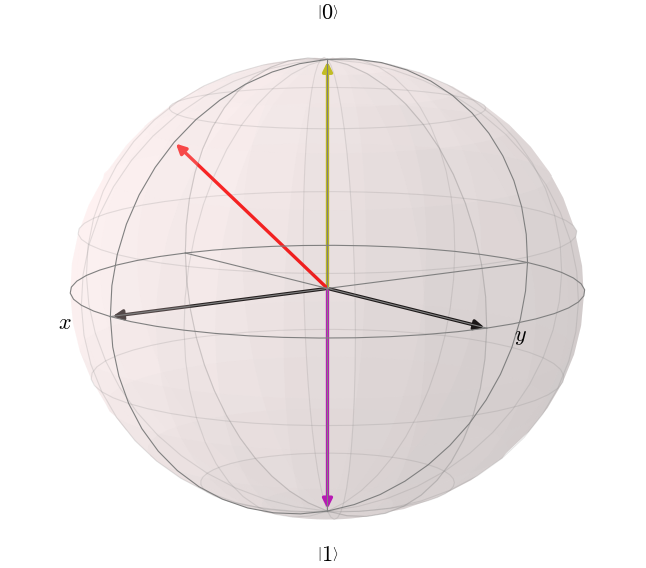
\includegraphics[scale=0.45]{img/3over4state.png}
       \caption{\label{fig:3over4}Visualisation of a simple binary classification problem of a quantum state vector on the Bloch sphere. The two training vectors are the \0 and \1 state coloured yellow and purple. The input state $e^{-i\frac{\pi}{8}}\big[0.92388\ket{0} + 0.38268\ket{1}\big]$ is shown in red.}
\end{figure}

\begin{minipage}[c]{.4\textwidth}
    \begin{tabular}{| C{0.8cm} | C{1.7cm} |C{2cm}|}
      \toprule
      Qubit state & Vector representation & Class\\
      \midrule
       $\ket{0}$ & $\colvec{1\\0}$ & $\ket{0}$ (yellow)\\\midrule
       $\ket{1}$ & $\colvec{0\\1}$ & $\ket{1}$ (purple)\\\midrule
      \bottomrule
    \end{tabular}
        \captionsetup{justification=justified, singlelinecheck=false}
    \captionof{table}{\label{tab:trainingset}Training dataset consisting of the two orthonormal states \0 and \1 with their respective class label.}
\end{minipage}%%%%
\hspace{0.5cm}
\begin{minipage}[c][][b]{.55\textwidth}
\flushright
    \begin{tabular}{| C{2.7cm} | C{2.3cm} |C{2cm}|}
      \toprule
      Qubit state & Vector representation & Expected class\\
      \midrule
       $e^{-i\frac{\pi}{8}}\big[0.92388\ket{0} + 0.38268\ket{1}\big]$ & $e^{-i\frac{\pi}{8}}\colvec{0.92388\\0.38268}$ & $\ket{0}$ (yellow)\\\midrule
      \bottomrule
    \end{tabular}
        \captionsetup{justification=justified, singlelinecheck=false}
    \captionof{table}{\label{tab:inputvectors}Input dataset containing a single state vector for the Bloch vector classification problem.}
\end{minipage}

\subsubsection{Initial state preparation}
\label{subsubsubsec:initialstatepreparation}

The first step towards an actual implementation of this problem is to prepare the initial quantum state $\ket{\psi_0}$ previously defined in Eq.~\ref{equ:ampinitial} to be of the form:
\begin{equation}
\label{equ:ampinitial2}
\ket{\psi_0} = \frac{1}{\sqrt{2M}}\sum_{m=1}^{M} (\ket{0}\ket{\textcolor{red}{\Psi_{x}}}+\ket{1}\ket{\textcolor{darkyellow}{\Psi}_{\textcolor{purple}{t^{m}}}})\ket{c^{m}}\ket{m}\, ,
\end{equation}
where in the case of the selected classification problem:
\begin{align} 
\label{equ:vectordefs}
&\ket{\textcolor{red}{\Psi_{x}}} = e^{-i\frac{\pi}{8}}\big[0.92388\ket{0} + 0.38268\ket{1}\big]\, ,\\
&\ket{\textcolor{darkyellow}{\Psi_{t^{1}}}} = \ket{0} \, ,\\
&\ket{\textcolor{purple}{\Psi_{t^{2}}}} = \ket{1}\, .
\end{align}
 
Since there are only two training vectors the index $m$ in Eq.~\ref{equ:ampinitial2} only takes the values 1 and 2. However, the $m$ qubit can only take binary values such that we need to redefine $1\rightarrow 0$ and $2\rightarrow 1$. With this observation, the required number of qubits can be deduced from Eq.~\ref{equ:ampinitial2}: one ancilla, one qubit for input and training vectors, one class qubit and one $m$ qubit making a total of four qubits. In the subsequent discussion the quantum state of the IBM QC in the $i^{th}$ step will be denoted $\ket{\chi_i}$. Since all qubits in the IBM Quantum Composer are initialised in state \0 the initial state $\ket{\chi_0}$ is simply:
\begin{equation}
\ket{\chi_0} = \ket{a}\ket{d}\ket{c}\ket{m} = \ket{0}\ket{0}\ket{0}\ket{0}\, ,
\end{equation}
where $a$ stands for ancilla, $d$ for data, $c$ for class and $m$ for the $m$ qubit. The sum over $m$ is introduced by simply acting an H gate on the $m$ qubit:
\begin{equation}
\label{equ:chi1}
\ket{\chi_1} = (\mathbb{1} \otimes \mathbb{1} \otimes \mathbb{1} \otimes H)\ket{0}\ket{0}\ket{0}\ket{0} = \frac{1}{\sqrt{2}} \sum_{m=0}^1 \ket{0}\ket{0}\ket{0}\ket{m}\, .
\end{equation}
%ADD CIRCUIT REPRESENTATION?
Using another H gate, the ancilla qubit is put in superposition:
\begin{equation}
\label{equ:chi2}
\ket{\chi_2} = (H \otimes \mathbb{1} \otimes \mathbb{1} \otimes \mathbb{1})\ket{\chi_1} = \frac{1}{2} \sum_{m=0}^1 \ket{0}\ket{0}\ket{0}\ket{m} + \ket{1}\ket{0}\ket{0}\ket{m} = \frac{1}{2} \sum_{m=0}^1 \big[ \ket{0}\ket{0} + \ket{1}\ket{0}\big] \ket{0}\ket{m}\, .
\end{equation}
%ADD CIRCUIT REPRESENTATION?

Next, the input vector $\ket{\textcolor{red}{\Psi_{x}}}$ should be loaded into the quantum state by means of a yet unknown gate sequence $GS$ such that the state is described by:
\begin{align}
\label{equ:chi3}
\ket{\chi_3} &= GS \ket{\chi_2} = \frac{1}{2} \sum_{m=0}^1 \big[ \ket{0}\ket{\textcolor{red}{\Psi_{x}}} + \ket{1}\ket{0}\big] \ket{0}\ket{m}\notag\\
&= \frac{1}{2} \sum_{m=0}^1 \Big[ \ket{0}\textcolor{red}{e^{-i\frac{\pi}{8}}\big[0.92388\ket{0} + 0.38268\ket{1}\big]} + \ket{1}\ket{0}\Big] \ket{0}\ket{m}\, .
\end{align}

By looking closely at Fig.~\ref{fig:3over4} one can deduce that the red input vector can be reached by simply rotating the \0 vector by an angle of $\frac{\pi}{4}$ around the y-axis. A y-rotation by an arbitrary angle $\vartheta$ can be achieved with the rotation operator $R_y(\vartheta)$. As described by \citeA{nielsen2010quantum}, $R_y(\vartheta)$ is obtained from exponentiating the Y gate and can be represented as the unitary 2x2 matrix:
\begin{equation}
\label{equ:rydef}
R_y(\vartheta) = e^{-i\vartheta\frac{Y}{2}} = \cos\frac{\vartheta}{2}\mathbb{1} - i\sin\frac{\vartheta}{2}Y \doteq \begin{pmatrix}
\cos\frac{\vartheta}{2} & -\sin\frac{\vartheta}{2} \\
\sin\frac{\vartheta}{2} & \cos\frac{\vartheta}{2}
\end{pmatrix}\, .
\end{equation}

As shown in Eq.~\ref{equ:chi3}, the input vector $\ket{\textcolor{red}{\Psi_{x}}}$ should only be entangled with the \0 state of the ancilla. To achieve this type of entanglement the controlled version of the y-rotation gate, $CR_y(\frac{\pi}{4})(c,t)$, is required. When applying it, using the $a$ qubit as control and the $d$ qubit as target, the input vector will be entangled with the \1 state of the ancilla. Flipping the $a$ qubit with an X gate moves the input vector to the \0 state of the ancilla. Hence, the desired state $\ket{\chi_3}$ is obtained by applying the following gate sequence $GS$:
\begin{equation}
\label{equ:gs}
GS = (X \otimes \mathbb{1} \otimes \mathbb{1} \otimes \mathbb{1}) (CR_y(\frac{\pi}{4})(a,d) \otimes \mathbb{1} \otimes \mathbb{1})\, . \\
\end{equation}
Substituting $GS$ into Eq.~\ref{equ:chi3} yields:
\begin{align}
\label{equ:chi3prepared}
\ket{\chi_3} &=  GS \ket{\chi_2} = (X \otimes \mathbb{1} \otimes \mathbb{1} \otimes \mathbb{1}) (CR_y(\frac{\pi}{4})(a,d) \otimes \mathbb{1} \otimes \mathbb{1}) \ket{\chi_2}\notag\\
&= (X \otimes \mathbb{1} \otimes \mathbb{1} \otimes \mathbb{1}) \Big[\frac{1}{2} \sum_{m=0}^1 \big[\ket{0}\ket{0} + \ket{1}\ket{\textcolor{red}{\Psi_{x}}}\big] \ket{0}\ket{m}\Big]\notag\\
&= \frac{1}{2} \sum_{m=0}^1 \Big[ \ket{0}\ket{\textcolor{red}{\Psi_{x}}} + \ket{1}\ket{0}\Big] \ket{0}\ket{m}\, .
\end{align}
At this point, note that $CR_y(\frac{\pi}{4})(c,t)$ is not an element of IBM's universal gate set. Its implementation on the IBM QC will be discussed in Section~\ref{subsubsubsec:controlledugate}.

%At this point, note that $R_y(\vartheta)$ is not an element of IBM's universal gate set. The problem of how to implement $R_y(\vartheta)$ on the IBM QC will be addressed later. For now, suppose $R_y(\frac{\pi}{4})$ can be implemented. Acting this gate on the data qubit in $\ket{\chi_2}$ yields the expression

%\begin{equation}
%(\mathbb{1} \otimes R_y(\frac{\pi}{4}) \otimes \mathbb{1} \otimes \mathbb{1})\ket{\chi_2} = \frac{1}{2} \sum_{m=0}^1 \big[ \ket{0}\ket{\textcolor{red}{\Psi_{x}}} + \ket{1}\ket{\textcolor{red}{\Psi_{x}}}\big] \ket{0}\ket{m}
%\end{equation}

%This, however, is not the desired state $\ket{\chi_3}$ defined in Eq.~\ref{equ:chi3} since 

The next step is to entangle the first training vector $\ket{\textcolor{darkyellow}{\Psi_{t^{0}}}}$  with the \1 state of the ancilla and the \0 state of the $m$ qubit. Additionally, the second training vector $\ket{\textcolor{purple}{\Psi_{t^{1}}}}$ should be entangled with the \1 states of the ancilla and the $m$ qubit. Note that $\ket{\textcolor{darkyellow}{\Psi_{t^{1}}}}$ and $\ket{\textcolor{purple}{\Psi_{t^{2}}}}$ defined in Eq.~\ref{equ:vectordefs} were redefined to $\ket{\textcolor{darkyellow}{\Psi_{t^{0}}}}$ and $\ket{\textcolor{purple}{\Psi_{t^{1}}}}$ respectively. Expanding the sum in Eq.~\ref{equ:chi3prepared} demonstrates that $\ket{\textcolor{darkyellow}{\Psi_{t^{0}}}} = \ket{0}$ is already at its desired place:
\begin{align}
\label{equ:chi3expanded}
\ket{\chi_3} &= \frac{1}{2}\Big[ \big[\ket{0}\ket{\textcolor{red}{\Psi_{x}}} + \ket{1}\ket{0}\big] \ket{0}\ket{0} + \big[ \ket{0}\ket{\textcolor{red}{\Psi_{x}}} + \ket{1}\ket{0}\big] \ket{0}\ket{1}\Big]\notag\\
&= \frac{1}{2}\Big[ \big[\ket{0}\ket{\textcolor{red}{\Psi_{x}}} + \ket{1}\ket{\textcolor{darkyellow}{\Psi_{t^{0}}}}\big] \ket{0}\ket{0} + \big[ \ket{0}\ket{\textcolor{red}{\Psi_{x}}} + \ket{1}\ket{0}\big] \ket{0}\ket{1}\Big]\, .
\end{align}

In order to entangle $\ket{\textcolor{purple}{\Psi_{t^{1}}}}$ with the \1 state of the ancilla and the $m$ qubit, a Toffoli (CCNOT) gate needs to be applied. Using the ancilla ($a$) and $m$ qubit as controls and choosing the data ($d$) qubit as target one obtains the following state:
\begin{align}
\label{equ:chi4}
\ket{\chi_4} &= CCNOT(a,m,d)\ket{\chi_3}\notag\\
&= \frac{1}{2}\Big[ \big[\ket{0}\ket{\textcolor{red}{\Psi_{x}}} + \ket{1}\ket{\textcolor{darkyellow}{\Psi_{t^{0}}}}\big] \ket{0}\ket{0} + \big[ \ket{0}\ket{\textcolor{red}{\Psi_{x}}} + \ket{1}\ket{1}\big] \ket{0}\ket{1}\Big]\notag\\
&= \frac{1}{2}\Big[ \big[\ket{0}\ket{\textcolor{red}{\Psi_{x}}} + \ket{1}\ket{\textcolor{darkyellow}{\Psi_{t^{0}}}}\big] \ket{0}\ket{0} + \big[ \ket{0}\ket{\textcolor{red}{\Psi_{x}}} + \ket{1}\ket{\textcolor{purple}{\Psi_{t^{1}}}}\big] \ket{0}\ket{1}\Big]\, .
\end{align}
Note again, that also the CCNOT gate is not an element of IBM's universal gate set which will be addressed later in Section~\ref{subsubsubsec:toffoli}.

\newpage
Eq.~\ref{equ:chi4} shows that the class qubit for the first training vector is already in the correct \0 state. It remains to flip the class qubit for the second training vector by applying a CNOT gate using the $d$ qubit as control and the class($c$) qubit as target. The resulting state is then defined by:
\begin{align}
\label{equ:chi5}
\ket{\chi_5} &= CNOT(d,c)\ket{\chi_4}\notag\\
&= \frac{1}{2}\Big[ \big[\ket{0}\ket{\textcolor{red}{\Psi_{x}}} + \ket{1}\ket{\textcolor{darkyellow}{\Psi_{t^{0}}}}\big] \ket{\textcolor{darkyellow}{0}}\ket{0} + \big[ \ket{0}\ket{\textcolor{red}{\Psi_{x}}} + \ket{1}\ket{\textcolor{purple}{\Psi_{t^{1}}}}\big] \ket{\textcolor{purple}{1}}\ket{1}\Big]\, ,
\end{align}
which can be rewritten as:
\begin{align}
\label{equ:chi5psi0}
\ket{\chi_5} &= \frac{1}{2} \sum_{m=1}^{2} \big[\ket{0}\ket{\textcolor{red}{\Psi_{x}}} + \ket{1}\ket{\textcolor{darkyellow}{\Psi_{t^{0}}}}\big] + \big[ \ket{0}\ket{\textcolor{red}{\Psi_{x}}} + \ket{1}\ket{\textcolor{purple}{\Psi_{t^{1}}}}\big]\ket{c^{m}}\ket{m}\notag\\
&= \frac{1}{2} \sum_{m=1}^{2} \big[\ket{0}\ket{\textcolor{red}{\Psi_{x}}} + \ket{1}\ket{\textcolor{darkyellow}{\Psi_{\textcolor{purple}{t^{m}}}}}\big]\ket{c^{m}}\ket{m}\, .
\end{align}

When comparing Eq.~\ref{equ:chi5psi0} to $\ket{\psi_0}$ in Eq.~\ref{equ:ampinitial} it becomes clear that $\ket{\chi_5}$ is in the form of the desired initial quantum state $\ket{\psi_0}$. The theoretical quantum state preparation is therefore completed. However, to implement the quantum state preparation on the IBM QC, it remains to find a way of realising the controlled y-rotation $CR_y(\frac{\pi}{4})(c,t)$ using only the ten gates from IBM's universal gate set. Hence, the focus of the following section will be to outline the necessary gate decomposition.

\subsubsection{Decomposition of a controlled-U gate}
\label{subsubsubsec:controlledugate}

In their book, \citeA{nielsen2010quantum} describe how a controlled U (CU) gate can be decomposed into a sequence of CNOT and single qubit gates. Thereby, U can be any unitary single-qubit gate. A CU gate is then defined as:
\begin{equation}
CU = \begin{pmatrix}
 \mathbb{1} & 0 \\ 
 0 & U
 \end{pmatrix}\, .
\end{equation}

Most of the time the CU gate cannot be implemented directly since it is not element of the universal gate set at hand and it has to be realised through larger quantum circuits. Fig.~\ref{img:cudecomposition} shows the decomposition described by \citeA{nielsen2010quantum} into two CNOTs, three unitary single-qubit gates $A,B,C$ and a phase-adjusting matrix which will be denoted $P$ of the form:
\begin{equation}
P = \begin{pmatrix}
 1 & 0 \\ 
 0 & e^{i\alpha}
 \end{pmatrix}\, .
\end{equation}

\begin{figure}[ht]
   \centering
   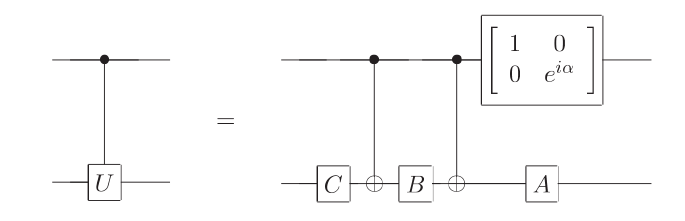
\includegraphics[width=0.7\textwidth]{img/controlledudecomp.png}
   \caption[]{Circuit decomposition of controlled-U quantum gate into two CNOTs, three unitary single-qubit gates $A$,$B$,$C$ and a phase-adjusting matrix.\footnotemark[15]}
   \label{img:cudecomposition}
\end{figure}

\footnotetext[15]{Reprinted from Michael A. Nielsen and Isaac L. Chuang. Quantum Computation and Quantum Information. Cambridge University Press, 2000. Copyright 2010 by Nielsen \& Chuang.}

The idea of this decomposition is, that when the control qubit (top qubit in Fig.~\ref{img:cudecomposition}) is \0 the gate combination $ABC$ is applied to the target qubit (bottom qubit in Fig.~\ref{img:cudecomposition}) and has to equal the identity gate:
\begin{equation}
\label{equ:abcidentity}
ABC = \mathbb{1}\, .
\end{equation}

If and only if the control qubit is \1 then the gate sequence $e^{i\alpha}AXBXC$ is applied to the target. Since the goal is to apply the unitary U to the target qubit the following equation must be satisfied:
\begin{equation}
\label{equ:UAXBXC}
e^{i\alpha}AXBXC = U\, .
\end{equation}
\citeA{nielsen2010quantum} make the following choices for the unitary gates $A,B,C$:
\begin{align}\label{equ:abc}
A &=  R_z(\beta)R_y(\frac{\gamma}{2})\, ,\\
B &= R_y(-\frac{\gamma}{2})R_z(-\frac{\delta+\beta}{2})\, ,\\
C &= R_z(\frac{\delta-\beta}{2})\, ,
\end{align}
where $R_z(\varrho)$ is the general rotation gate about the z-axis of the Bloch sphere. Similarly to the $R_y(\vartheta)$ gate it can be obtained by exponentiating the Z gate as shown below in Eq.~\ref{equ:rzdef}.
\begin{equation}
\label{equ:rzdef}
R_z(\varrho) = e^{-i\varrho\frac{Z}{2}} = \cos\frac{\varrho}{2} \mathbb{1}- i\sin\frac{\varrho}{2}Z = \begin{pmatrix}
e^{-i\frac{\varrho}{2}} & 0 \\
0 & e^{i\frac{\varrho}{2}}
\end{pmatrix}\, .
\end{equation}

When substituting the expressions for $A,B,C$ from Eq.~\ref{equ:abc} into Eq.~\ref{equ:abcidentity} one will indeed obtain the identity operation as shown by \citeA{nielsen2010quantum}(proof omitted). These choices of $A,B,C$ are also a solution to Eq.~\ref{equ:UAXBXC}. Substituting into Eq.~\ref{equ:UAXBXC} leads to the following expression for matrix $U$:
\begin{equation}
\label{equ:udecompdef}
U = \begin{pmatrix}
 e^{i(\alpha-\frac{\beta}{2}-\frac{\delta}{2})}\cos{\frac{\gamma}{2}} & -e^{i(\alpha-\frac{\beta}{2}+\frac{\delta}{2})}\sin{\frac{\gamma}{2}} \\ 
e^{i(\alpha+\frac{\beta}{2}-\frac{\delta}{2})}\sin{\frac{\gamma}{2}} & e^{i(\alpha+\frac{\beta}{2}+\frac{\delta}{2})}\cos{\frac{\gamma}{2}}
 \end{pmatrix}\, .
\end{equation}
%Furthermore, \citeA{nielsen2010quantum} show that any unitary matrix U can be decomposed as,
%\begin{equation}
%\label{equ:URzRyRz}
%U = e^{i\alpha}R_z(\beta)R_y(\gamma)R_z(\delta)
%\end{equation}
%\begin{equation}
%\label{equ:UAXBXC}
%e^{i\alpha}AR_x(\pi)BR_x(\pi)C = U
%\end{equation}

To decompose $CR_y(\frac{\pi}{4})$, one simply chooses $U = R_y(\frac{\pi}{4})$. By substituting $\vartheta = \frac{\pi}{4}$ into Eq.~\ref{equ:rydef} the matrix representation of $R_y(\frac{\pi}{4})$ is obtained:
\begin{equation}
U = R_y(\frac{\pi}{4}) = \begin{pmatrix}
\cos\frac{\pi}{8} & -\sin\frac{\pi}{8} \\
\sin\frac{\pi}{8} & \cos\frac{\pi}{8}
\end{pmatrix}\, .
\end{equation}
Substituting this expression for $U$ into Eq.~\ref{equ:udecompdef} leads to:
\begin{equation}
\label{equ:udecompsubbed}
U = \begin{pmatrix}
\cos\frac{\pi}{8} & -\sin\frac{\pi}{8} \\
\sin\frac{\pi}{8} & \cos\frac{\pi}{8}
\end{pmatrix} = \begin{pmatrix}
 e^{i(\alpha-\frac{\beta}{2}-\frac{\delta}{2})}\cos{\frac{\gamma}{2}} & -e^{i(\alpha-\frac{\beta}{2}+\frac{\delta}{2})}\sin{\frac{\gamma}{2}} \\ 
e^{i(\alpha+\frac{\beta}{2}-\frac{\delta}{2})}\sin{\frac{\gamma}{2}} & e^{i(\alpha+\frac{\beta}{2}+\frac{\delta}{2})}\cos{\frac{\gamma}{2}}
 \end{pmatrix}\, .
\end{equation}

\newpage
When setting the expressions for the respective matrix entries in Eq.~\ref{equ:udecompsubbed} equal, the following system of non-linear complex equations is obtained :
\begin{align}
\label{equ:nlsystem}
\cos\frac{\pi}{8} &= e^{i(\alpha-\frac{\beta}{2}-\frac{\delta}{2})}\cos{\frac{\gamma}{2}}\, ,\\
\sin\frac{\pi}{8} &= e^{i(\alpha-\frac{\beta}{2}+\frac{\delta}{2})}\sin{\frac{\gamma}{2}}\, ,  \\
\sin\frac{\pi}{8} &= e^{i(\alpha+\frac{\beta}{2}-\frac{\delta}{2})}\sin{\frac{\gamma}{2}}\, ,\\
\cos\frac{\pi}{8} &= e^{i(\alpha+\frac{\beta}{2}+\frac{\delta}{2})}\cos{\frac{\gamma}{2}}\, .
\end{align}


This is a system of four non-linear complex equations with four unknowns. In order to solve for the parameters $\alpha,\beta,\gamma$ and $\delta$ one can use any root finding algorithm for non-linear equations such as Secant or Newton's method. Using Newton's method the solutions are found to be:
\begin{equation}
\alpha =  \pi; \quad 
\beta = 2\pi;\quad 
\delta = \frac{7}{8}\pi;\quad 
\gamma = 0\, .
\end{equation}
Substituting these parameters into the expressions for $A,B$ and $C$ defined in Eq.~\ref{equ:abc} yields:
\begin{align}
\label{equ:abcsubbed1}
A \quad= \quad R_z(\beta)R_y(\frac{\gamma}{2})\quad =& \quad R_z(2\pi) \quad = \quad \textcolor{emerald}{\mathbb{1}}\, , \\
\label{equ:abcsubbed2}
B\quad =\quad R_y(-\frac{\gamma}{2})R_z(-\frac{\delta+\beta}{2})\quad =& \quad R_z(-\frac{23}{16}\pi) \quad= \quad \textcolor{red}{?} \, ,\\
\label{equ:abcsubbed3}
C \quad=\quad R_z(\frac{\delta-\beta}{2})\quad =& \quad R_z(-\frac{9}{16}\pi) \quad= \quad \textcolor{red}{?}\, , \\
\label{equ:abcsubbed4}
P\quad =\quad \begin{pmatrix} 1&0\cr0&e^{i\alpha} \end{pmatrix}\quad=& \quad \begin{pmatrix} 1&0\cr0&e^{i\pi} \end{pmatrix}\quad= \quad \textcolor{emerald}{Z}\, .
\end{align}


Quantum gate $A$ is just equal to the identity gate which certainly is an element of IBM's universal gate set. The phase-adjusting gate $P$ is equal to the Z gate that also is within IBM's gate set. Only gates $B$ and $C$ result in more complex z-rotations of $-\frac{23}{16}\pi$ and $-\frac{9}{16}\pi$ radians respectively. Unfortunately, these quantum gates are not found in IBM's gate set as indicated by the red question marks in Eq.~\ref{equ:abcsubbed2} and \ref{equ:abcsubbed3}. The further decomposition of these z-rotations will be the focus of the next section.

\subsubsection{The Solovay-Kitaev theorem}
\label{subsubsubsec:solovaykitaev}

An important theorem in quantum information is the Solovay-Kitaev theorem first proposed by Solovay and later published by \citeA{kitaev1995quantum}. It will be used to decompose the quantum gates $B$ and $C$ into a sequence of quantum gates from IBM's universal gate set. At this point, it is important to remember that any universal quantum gate set is a dense subset of the special unitary group $\mathrm{SU}(2)$ as previously defined in Section~\ref{subsubsec:qubits}.
\vspace{0.3cm}
\begin{redbox}
\textbf{Theorem: Solovay-Kitaev theorem}\\
\newline
Let $G$ be a universal quantum set $G$ consisting of quantum gates from $\mathrm{SU}(2)$ and let $\epsilon > 0$ be a desired accuracy. Then there is a constant $b$ such that for any single-qubit gate $W \in \mathrm{SU}(2)$ there exists a
finite gate sequence $\tilde{G}$ of gates from the set $G$ of length $O(\log^b (1/\epsilon))$ such that $d(W, \tilde{G}) < \epsilon$. In their proof, \citeA{dawson2005solovay} show that $b \approx 3.97$.\\
\newline
In other words, given a set of single-qubit quantum gates which is a dense subset of $\mathrm{SU}(2)$, then the Solovay-Kitaev theorem guarantees that this set will quickly fill $\mathrm{SU}(2)$.
\cite{dawson2005solovay}.
\end{redbox}
%\vspace{0.2cm}
The importance of the Solovay-Kitaev theorem arises from proving that given any universal gate set it is possible to obtain good approximations to any desired single-qubit gate $W$. In their paper, \citeA{dawson2005solovay} describe how to design an algorithm implementing the Solovay-Kitaev theorem. Unfortunately, the Solovay-Kitaev algorithm needs to be implemented on a classical computer which adds to the overall time complexity of the quantum compiling process as will be shown later. For this thesis, the open-source software package 'Quantum Compiler, v0.03'\footnotemark[16] developed in Python by Paul Pham was used to run the Solovay-Kitaev algorithm described by \citeA{dawson2005solovay}. This software package compares different gate approximations to the desired gate by a new distance metric called Fowler distance.

\footnotetext[16]{The software package 'Quantum Compiler, v0.03' by Paul Pham can be downloaded from \url{https://sourceforge.net/projects/quantumcompiler/files/v0.03/}.}

\begin{redbox}
\textbf{Definition: Fowler distance}\\
\newline
When approximating a unitary gate $W$ with a gate sequence yielding another unitary gate $W_\mathrm\mathrm{approx}$ it is important to quantify how 'close' the action of $W_\mathrm{approx}$ is to $W$. The Fowler distance makes use of the matrix representations of $W$ and $W_\mathrm{approx}$ and is defined by \citeA{booth2012quantum} as:
\begin{equation}
d(W,W_\mathrm{approx}) = \sqrt{\frac{2-\mid tr(W\cdot W_{\mathrm\mathrm{approx}}^\dagger)\mid}{2}}
\end{equation}

In contrast to $W$, $W_\mathrm{approx}$ might introduce a shift in the global phase of the quantum state it is acting on. However, since a global phase of a quantum state is immeasurable in experiment, it can be neglected \cite{nielsen2010quantum}. As a result, the Fowler distance is defined in such a way that possible global phase differences are ignored.
\end{redbox}

Subsequently, the desired gates $B = R_z(-\frac{23}{16}\pi)$ and $C = R_z(-\frac{9}{16}\pi)$ where decomposed using the Solovay-Kitaev algorithm. Fig.~\ref{fig:skresultplot} shows a plot visualising how the Fowler distance depends on the number of gates in the approximating gate sequence $W_\mathrm{approx}$. The number of gates in the approximating gate sequence is also called \emph{gate count}. The plot clearly shows an exponential increase in the gate count for decreasing Fowler distance. For example, 146 gates suffice to achieve $d(W_\mathrm{approx},R_z(-\frac{9}{16}\pi)) = 0.04389$. Yet, already 17,838 gates are required to reduce the Fowler distance to $d(W_\mathrm{approx},R_z(-\frac{9}{16}\pi)) = 0.01008$.

\begin{figure}[H]
\centering
    \begin{tikzpicture}[scale=0.85]
\begin{axis}[xlabel={Gate count},ylabel={Fowler distance [$d(U,U_{approx})$]}]

% Graph column 2 versus column 0
\addplot table[x index=1,y index=0,col sep=comma] {datax.dat};
\addlegendentry{$R_z(-\frac{9}{16}\pi)$}% y index+1 since humans count from 1

% Graph column 1 versus column 0    
\addplot table[x index=5,y index=4,col sep=comma] {datax.dat};
\addlegendentry{$R_z(-\frac{23}{16}\pi)$}

\end{axis}
\end{tikzpicture}
\caption{Fowler distance plotted against the required gate count for quantum gates $B = R_z(-\frac{23}{16}\pi)$ and $C = R_z(-\frac{9}{16}\pi)$. The plot shows an exponential increase in the gate count with decreasing Fowler distance.}
\label{fig:skresultplot}
  \end{figure}

\begin{figure}[H]
\centering
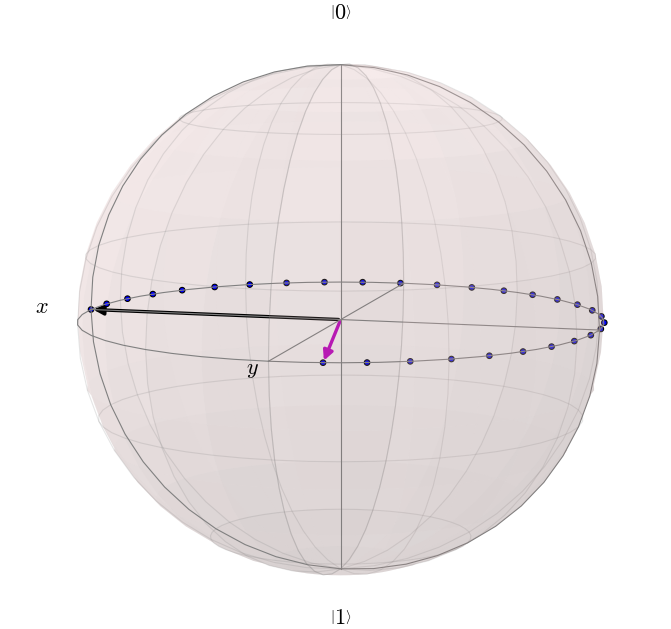
\includegraphics[scale=0.38]{img/bloch23over16.png}
\caption{\label{fig:bloch23over16} Applying $B = R_z(-\frac{23}{16}\pi)$ to the state $\ket{\psi} = \frac{\ket{0} + \ket{1}}{\sqrt{2}}$ leads to the purple vector $\vec{b}$. The plot shows the rotation of $-\frac{23}{16}\pi$ radians around the $\hat{z}$-axis of the Bloch sphere.}
\end{figure}
Fowler distance is best understood with a visual example using the gate $B = R_z(-\frac{23}{16}\pi)$. Acting the desired gate $B$ on the state $\ket{\psi} = \frac{\ket{0} + \ket{1}}{\sqrt{2}}$ (black vector in Fig.~\ref{fig:bloch23over16}) results in the purple Bloch vector $\vec{b}$ shown in Fig.~\ref{fig:bloch23over16}. In comparison, Fig.~\ref{fig:fowlerdistances} shows the action of four different approximating gate sequences $B_\mathrm{approx,1}$, $B_\mathrm{approx,2}$, $B_\mathrm{approx,3}$, $B_\mathrm{approx,4}$ on the state $\ket{\psi} = \frac{\ket{0} + \ket{1}}{\sqrt{2}}$.
\begin{minipage}[c]{.8\textwidth}
    %\vspace{-20mm}
    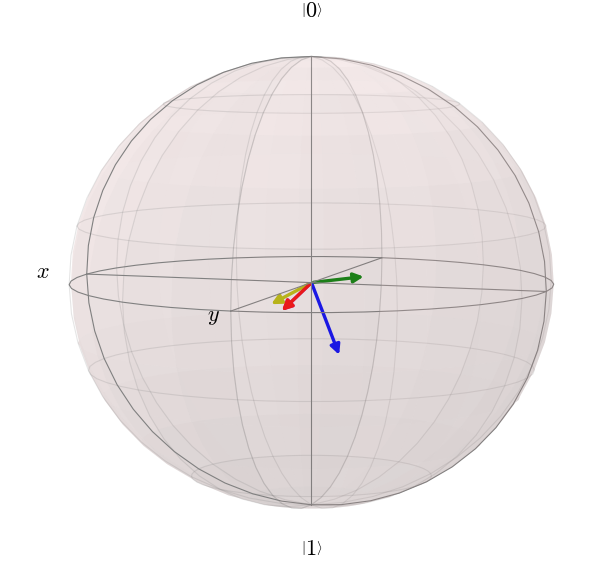
\includegraphics[height=0.7\textwidth]{img/fowlerdistances.png}
       \captionsetup{justification=raggedright, singlelinecheck=false}
       \captionof{figure}{\label{fig:fowlerdistances}Visualisation of the obtained state vectors from the action of gate sequences $B_\mathrm{approx,1}$, $B_\mathrm{approx,2}$, $B_\mathrm{approx,3}$, $B_\mathrm{approx,4}$ onto the state $\ket{\psi} = \frac{\ket{0} + \ket{1}}{\sqrt{2}}$. The plot visually shows the difference between different Fowler distances on the Bloch sphere.}
\end{minipage}%%%%%
\begin{minipage}[c]{.2\textwidth}
\begin{equation}
\textcolor{emerald}{d(B,B_\mathrm{approx,1}) = 0.15165} \notag
\end{equation}
\begin{equation}
\textcolor{blue}{d(B,B_\mathrm{approx,2}) = 0.10722} \notag
\end{equation}
\begin{equation}
\textcolor{darkyellow}{d(B,B_\mathrm{approx,3}) = 0.02086} \notag
\end{equation}
\begin{equation}
\textcolor{red}{d(B,B_\mathrm{approx,4}) = 0.00158} \notag
\end{equation}
\end{minipage}

Gate sequence $B_\mathrm{approx,1}$ consists of 25 gates and is a Fowler distance of $d = 0.15165$ away from $B$. The resulting state vector is coloured green in Fig.~\ref{fig:fowlerdistances}. The green vector lies above the Bloch equator and is relatively far away from the desired vector $\vec{b}$ in Fig.~\ref{fig:bloch23over16}. With 109 gates, $B_\mathrm{approx,2}$ yields a Fowler distance of $d = 0.10722$ resulting in the blue vector. It can be seen, that the blue state vector lies below the Bloch equator and is still relatively far from $\vec{b}$. Using $B_\mathrm{approx,3}$ the Fowler distance drops to $d = 0.02086$ leading to the yellow vector in  Fig.~\ref{fig:fowlerdistances}. This yellow vector is almost on the Bloch equator and relatively close to $\vec{b}$ implying that $B_\mathrm{approx,3}$ is a good approximation of $B$. However, $B_\mathrm{approx,3}$ already requires the implementation of 2,997 single-qubit gates. The purple vector from Fig.~\ref{fig:bloch23over16} is also plotted in Fig.~\ref{fig:fowlerdistances} but is not visible since the red vector with $d = 0.00158$ constitutes a very good approximation to the desired state $\vec{b}$.  The red vector is the result of the action of $B_\mathrm{approx,4}$ which, unfortunately, needs 370,813 gates to achieve such a small Fowler distance. Hereby, Gate $B$ was used as an example but such an exponential increase in the gate count is observed for any quantum gate $W$ when applying the Solovay-Kitaev algorithm \cite{dawson2005solovay}.

Implementing any quantum gate $D$ inevitably takes some time $t$ since it involves the use of hardware components e.g. targeting a specific atom with a laser pulse. Based on IBM's single-qubit and CNOT gate times described in Section~\ref{subsec:ibmqc} the total execution time of twelve different gate sequences, approximating $B = R_z(-\frac{23}{16}\pi)$ and $C = R_z(-\frac{9}{16}\pi)$ to different Fowler distances, were calculated. The results can be seen in Table~\ref{tab:sktimes}. Keeping in mind that in the best case, the maximum decoherence time of a qubit in IBM's QC is \SI{112.4}{\micro\second} most gate sequences are too long for an IBM implementation (coloured red in Table~\ref{tab:sktimes}). Feasible execution times are marked green in Table~\ref{tab:sktimes}. However, decoherence is not the only limiting factor since IBM only allows for 39 gates and one measurement gate per qubit. Even when selecting the smallest sequences of 25 gates for $B$ and 16 gates for $C$, the total gate count is 41 which is two gates more than the allowed gate count of the IBM Quantum Composer. Note that the approximating gate sequences of $B$ and $C$ are not the only gates needed to prepare the initial quantum state and execute the akNN algorithm. Unfortunately, this makes an actual implementation of this particular classification problem on IBM's present QC impossible. However, to complete the quantum compiling, assume that gates $B$ and $C$ could somehow be implemented with shorter gate sequences. For the following section, it remains to decompose the Toffoli gate that was required to 'load' the second training pattern $\ket{\textcolor{purple}{\Psi_{t^{1}}}}$ into the quantum state $\ket{\chi_4}$ as shown in Eq.~\ref{equ:chi4}.

%Thus, the only possibility would be to select the sequence of 25 gates for $B$ and the sequence of 16 gates for $C$ at the cost of relatively large Fowler distances. This, however, still sums up to 41 gates which are two gates more than the allowed gate count of the IBM Quantum Composer. 
\begin{table}[H]
\centering
    \begin{tabular}{c| c |c |c }
      \toprule
      Approx. Gate & Fowler distance & Gate count & Execution time\\
      \midrule
      $R_z(-\frac{23}{16}\pi)$ & 0.15165 & 25 & \textcolor{emerald}{$\sim$\SI{3}{\micro\second}}\\
       & 0.10722 & 109 & \textcolor{emerald}{$\sim$\SI{14}{\micro\second}}\\
       & 0.02086 & 2,997 & \textcolor{red}{$\sim$\SI{390}{\micro\second}}\\
       & 0.01494 & 14,721 & \textcolor{red}{$\sim$\SI{1914}{\micro\second}}\\
       & 0.003327 & 74,009 & \textcolor{red}{$\sim$\SI{9621}{\micro\second}}\\
       & 0.001578 & 370,813 & \textcolor{red}{$\sim$\SI{48206}{\micro\second}}\\
       \midrule
      $R_z(-\frac{9}{16}\pi)$ & 0.28390 & 16 & \textcolor{emerald}{$\sim$\SI{2}{\micro\second}}\\
       & 0.04389 & 146 & \textcolor{emerald}{$\sim$\SI{18}{\micro\second}}\\
       & 0.049511 & 728 & \textcolor{emerald}{$\sim$\SI{87}{\micro\second}}\\
       & 0.02823 & 3,622 & \textcolor{red}{$\sim$\SI{435}{\micro\second}}\\
       & 0.01008 & 17,838 & \textcolor{red}{$\sim$\SI{2141}{\micro\second}}\\
       & 0.00156 & 444,646 & \textcolor{red}{$\sim$\SI{53358}{\micro\second}}\\
      \bottomrule
      \bottomrule
    \end{tabular}
    \caption{\label{tab:sktimes} The table shows the Fowler distance and gate count for different gate sequences approximating the gates $B = R_z(-\frac{23}{16}\pi)$ and $C = R_z(-\frac{9}{16}\pi)$ after decomposition with the Solovay-Kitaev algorithm. The execution time for each gate sequence was calculated by multiplying the gate count with IBM's single-qubit gate time of 130ns.}
  \end{table}

\subsubsection{Toffoli Gate Decomposition}
\label{subsubsubsec:toffoli}

The Toffoli or CCNOT gate can be decomposed into CNOT and single-qubit gates in several ways. In their book, \citeA{nielsen2010quantum} describe the decomposition into six CNOTs and nine single-qubit gates; two H gates, three T and three T$^\dagger$ gates. See Fig.~\ref{img:toffolidecomp} for the corresponding circuit diagram. This decomposition does not require any further compiling work since all involved gates are elements of IBM's universal gate set.

\begin{figure}[!ht]
       \centering
       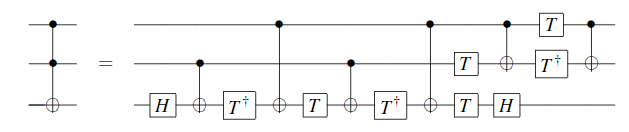
\includegraphics[scale=0.5]{img/toffolidecomposition.png}
       \caption[]{\label{img:toffolidecomp} Decomposition of a Toffoli gate into six CNOT and nine single-qubit gates\footnotemark[17]}
\end{figure}

\footnotetext[17]{Reprinted from Michael A. Nielsen and Isaac L. Chuang. Quantum Computation and Quantum Information. Cambridge University Press, 2000. Copyright 2010 by Nielsen \& Chuang.}

The Toffoli decomposition finalises the compiling of the quantum state preparation into gates from IBM's gate set only. In summary, the compiled state preparation requires: 
\begin{itemize}
\item 2 H gates applied to the ancilla and the $m$ qubit
\item the decomposed $CR_y(\frac{\pi}{4})$ gate (2 CNOTs, 1 Z gate, 1 $\mathbb{1}$ gate (can be neglected) \& a sequence of minimum 25 gates for $B$ and minimum 16 gates for $C$)
\item 1 X gate to flip the ancilla (Eq.~\ref{equ:chi3prepared})
\item 1 decomposed Toffoli (6 CNOTs, 2 H gates, 3 T \& 3 T$^\dagger$ gates) to load the second training vector
\item 1 CNOT to flip the class qubit
\end{itemize}
Thus, the quantum state preparation was compiled into 9 CNOT and 53 single-qubit gates. The akNN algorithm only requires one additional H gate and two measurement gates (for ancilla and class qubit) leading to a total of 9 CNOT, 54 single-qubit gates and two measurement gates. However, even cleverly arranging these gates does not suffice to implement the algorithm within IBM's 40 gate slots. The full circuit diagram for the compiled state preparation and the aKNN algorithm can be seen in Fig.~\ref{img:toffolidecomp}.

\begin{figure}[!ht]
       \centering
       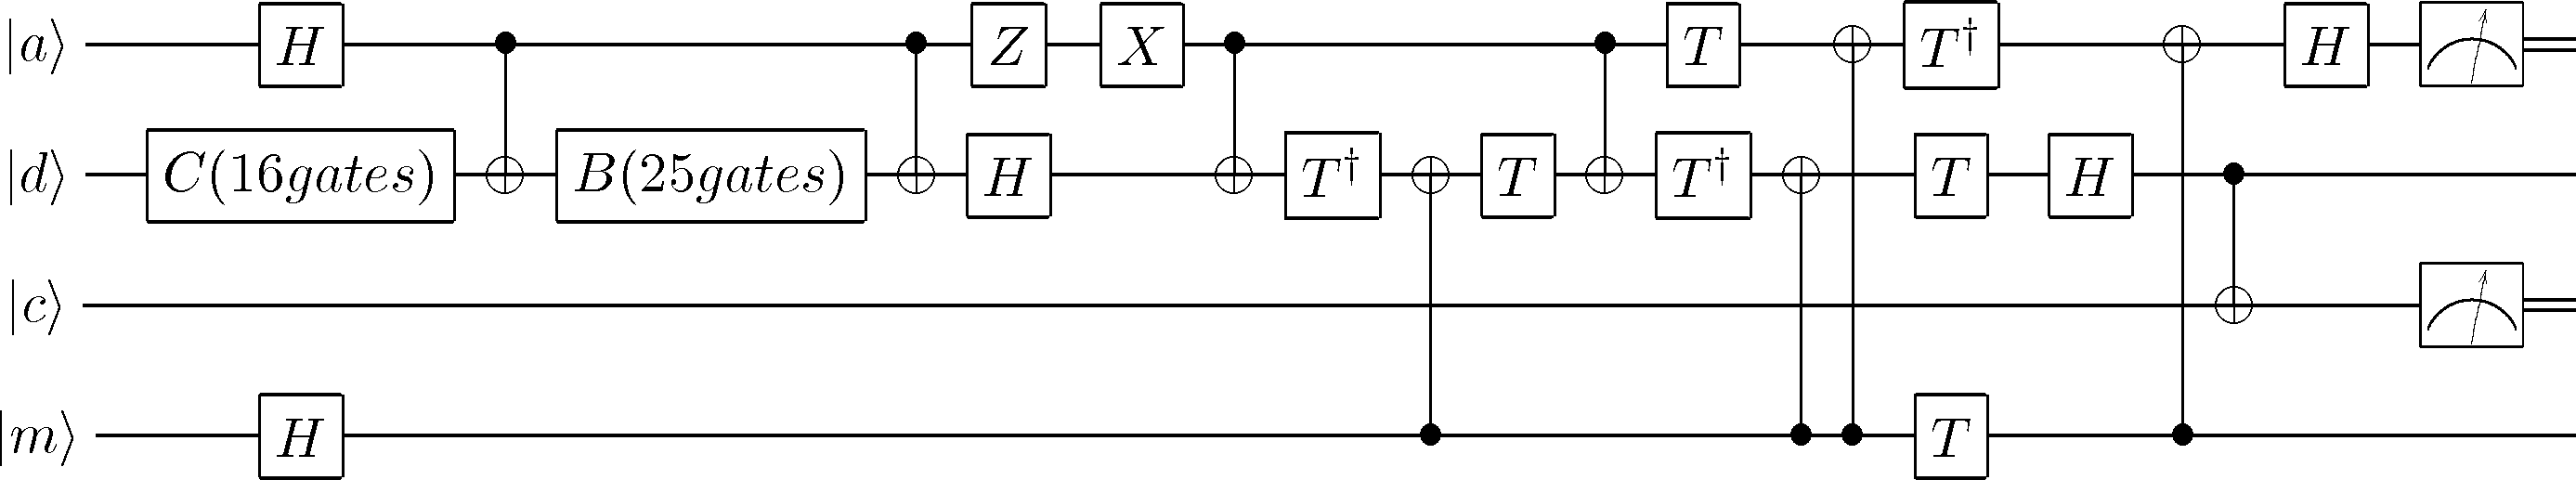
\includegraphics[width=\textwidth]{img/fullQKNN.png}
       \caption[]{\label{img:toffolidecomp} Compiled quantum circuit implementating the aKNN algorithm for the binary Bloch vector classification problem.}
\end{figure}

%state preparation
%H Gate m qubit
%H Gate ancilla
%CR_y decomposed
%X Gate ancilla
%Toffoli(a,m,d)
%CNOT(d,c)
%algorithm
%H ancilla
%CM ancilla
%M class
%Final circuit diagram showing the compile state preparation + akNN algorithm steps

\begin{greenbox}
\textbf{Complexity analysis including quantum compiling steps}\\
\newline
The amplitude-based kNN algorithm itself was found to run in constant time $\mathcal{O}(\frac{1}{\mathrm{Prob(CM)}})$. However, to determine the overall algorithmic complexity all steps required to prepare the initial quantum state $\ket{\psi_0}$ from Eq.~\ref{equ:ampinitial} need to be included. The decomposition of the $CR_y(\frac{\pi}{4})$ gate involved solving a system of non-linear equations by means of a root-finding algorithm. Any iterative root-finding algorithm e.g. Secant or Newton's method has a complexity of $\mathcal{O}(k)$ where $k$ is the number of root finding iterations. Furthermore, the Solovay-Kitaev algorithm was required to find two single-qubit gate sequences approximating the two gates $B = R_z(-\frac{23}{16}\pi)$ and $C = R_z(-\frac{9}{16}\pi)$. According to \citeA{dawson2005solovay} the Solovay-Kitaev algorithm has a complexity of $\mathcal{O}(m\cdot \log^{2.71}(\frac{m}{\epsilon}))$ for $\epsilon$-approximations of $m$ gates. Thus the total complexity is given by:
\begin{equation}
\mathcal{O}(\frac{1}{\mathrm{Prob(CM)}})+\mathcal{O}(k)+\mathcal{O}(m\cdot \log^{2.71}(\frac{m}{\epsilon}))
\end{equation}
    
When adding algorithmic complexities only the most dominant term is considered relevant. Thus, the overall complexity including state preparation is found to be $\mathcal{O}(m\cdot \log^{2.71}(\frac{m}{\epsilon}))$.\\
\newline
In conclusion, due to the necessary quantum compiling steps the initial constant complexity of the akNN algorithm
\begin{equation}  
\mathcal{O}(\frac{1}{\mathrm{Prob(CM)}})
\end{equation}
increased to a polylogarithmic complexity of
\begin{equation}
\mathcal{O}(m\cdot \log^{2.71}(\frac{m}{\epsilon}))
\end{equation}
dependening on the number of gates $m$ that need $\epsilon$-approximations by means of the Solovay-Kitaev algorithm.
\end{greenbox}

All in all, it is important to note that the input vector $e^{-i\frac{\pi}{8}}\big[0.92388\ket{0} + 0.38268\ket{1}\big]$ was chosen as an illustrative example. The quantum compiling steps necessary to initialise this input vector cannot be generalised to other state vectors on the Bloch sphere. There might be state vectors that are much easier to prepare and which do not result in long decomposed gate sequences. On the other hand, there might also be many state vectors that are as or even more difficult to prepare than the presented input vector. Yet, it is important to keep in mind that in the field of quantum machine learning, one cannot just select training and input vectors that can easily be encoded into quantum states since this would introduce a strong bias into the data. This becomes especially important when considering that QML aims to provide speedups with respect to big data processing. Big data can involve millions or billions of training vectors of which many might be difficult to encode into quantum states. Despite the fact, that this example cannot be formally generalised to other state vectors, it still demonstrated the general quantum compiling procedure required to implement the Bloch vector classification problem using IBM's universal gate set.

%All in all, it was shown that for this particular classification problem the constant complexity of the aKNN algorithm is dominated by the complexity of the quantum compiling. 

\subsection{Simulating the amplitude-based kNN algorithm}
\label{subsubsec:simulationamplitudeKNN}

Since the IBM Quantum Experience does not allow for an implementation, the aKNN algorithm was simulated in Liqui$\ket{}$ to determine the performance and the outcome of the algorithm. This section is subdivided into two parts: First, the classification of Bloch vectors described in the previous section is simulated. Second, the aKNN algorithm is used to classify different Gaussian distributions, thereby, constituting a slightly more complex classification task.

\begin{figure}[H]
       \centering
       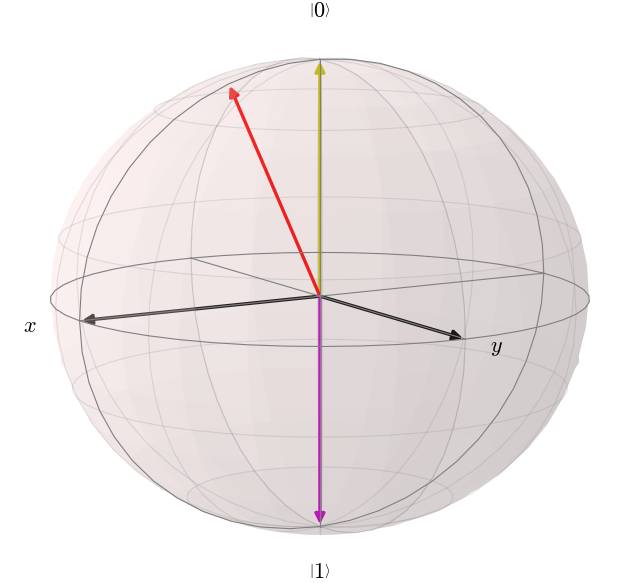
\includegraphics[scale=0.35]{img/bloch7over8.png}
       \caption{\label{img:7over8} Visualisation of the second input qubit state $e^{-i\frac{\pi}{16}}\big[0.98079\ket{0} + 0.19509\ket{1}\big]$ coloured red on the Bloch sphere. The first training vector \0 is shown in yellow and the second training vector \1 is shown in purple.}
\end{figure}

\subsubsection{Classification of Bloch vectors}
\label{subsubsubsec:classificationblochvectors}

The Bloch vector classification problem described in Section~\ref{subsubsec:implementationamplitudeKNN} was reconsidered and simulated in Liqui$\ket{}$ to determine if the algorithm yields the expected classification outcome. Section~\ref{subsubsec:implementationamplitudeKNN} pointed out that the implementation of the controlled y-rotation $CR_y(\frac{\pi}{4})$ was the main issue preventing an implementation within IBM's 40 gate slots. However, by specifying its matrix representation, Liqui$\ket{}$ allows any unitary single- or multi-qubit gate to be defined within its programming framework. Therefore, $CR_y(\frac{\pi}{4})$ can be easily implemented in Liqui$\ket{}$. This enables loading the input vector specified in Table~\ref{tab:inputvectors} without having to decompose the controlled y-rotation gate and with no need for the Solovay-Kitaev algorithm. Due to this enormous simplification of the quantum state preparation routine, a second input vector was considered for simulation. Fig.~\ref{img:7over8} shows the new second input vector on the Bloch sphere. This new input vector can be obtained by rotating the \0 state by $\frac{\pi}{8}$ radians around the y-axis. The resulting new input dataset is listed in Table~\ref{tab:inputvectors2}.

\begin{table}[H]
\centering
\begin{tabular}{| C{0.5cm} | C{2.7cm} | C{2.3cm} |C{2cm}|}
      \toprule
      ID & Qubit state & Vector representation & Expected class\\
      \midrule
       1 & $e^{-i\frac{\pi}{8}}\big[0.92388\ket{0} + 0.38268\ket{1}\big]$ & $e^{-i\frac{\pi}{8}}\colvec{0.92388\\0.38268}$ & $\ket{0}$ (yellow)\\\midrule
       2 & $e^{-i\frac{\pi}{16}}\big[0.98079\ket{0} + 0.19509\ket{1}\big]$ & $e^{-i\frac{\pi}{16}}\colvec{0.98079\\0.19509}$ & $\ket{0}$ (yellow)\\\midrule
      \bottomrule
    \end{tabular}
    \caption{\label{tab:inputvectors2} Input dataset II for the simulation of the aKNN algorithm. The dataset consists of two different qubit states both lying in the z-x plane of the Bloch sphere.}
\end{table}

\newpage
Table~\ref{tab:inputvectors2} shows that the probability of measuring the new input vector (ID 2) in state \0 is slightly higher than for the first input vector (ID 1). This can also be seen visually when comparing Fig.~\ref{img:7over8} to Fig.~\ref{fig:3over4}: the second input vector (ID 2) is closer to the \0 state than the first input vector (ID 1). For the quantum simulation, the training dataset listed in Table~\ref{tab:trainingset} was not changed.

The obtained simulation results after 1000 runs for both Bloch vectors from input dataset II are shown in Table~\ref{tab:blochresults}. The theoretically predicted probabilities are marked with asterisks and are always displayed on top of the corresponding simulation results. Comparing these values shows strong agreement between prediction and simulation and the expected maximum error of $\frac{1}{\sqrt{1000}}=0.03$ is not exceeded. 

\begin{table}[H]
\begin{tabular}{| C{0.5cm} | C{2.7cm} |C{1.7cm} | C{1.7cm} | C{1.7cm} |C{1.8cm}| C{1.8cm}|}
      \toprule
      ID & Vector representation  & $\mathrm{Prob(CM)}$ & $\mathrm{Prob}$ $(\ket{c} = \ket{0})$ & $\mathrm{Prob}$ $(\ket{c} = \ket{1})$ & Expected class & Algorithm output\\
      \midrule
        1 & $e^{-i\frac{\pi}{8}}\colvec{0.92388\\0.38268}$ & \begin{tabular}{c} 0.8266* \\\midrule 0.8050 \end{tabular} & \begin{tabular}{c} 0.5818* \\\midrule 0.5863 \end{tabular} & \begin{tabular}{c} 0.4182* \\\midrule 0.4137 \end{tabular} & $\ket{0}$ (yellow) & $\ket{0}$ (yellow)\\\midrule
        
       2 & $e^{-i\frac{\pi}{16}}\colvec{0.98079\\0.19509}$ & \begin{tabular}{c} 0.7940* \\\midrule 0.7710 \end{tabular} & \begin{tabular}{c} 0.6237* \\\midrule 0.6420 \end{tabular} & \begin{tabular}{c} 0.3763* \\\midrule 0.3580 \end{tabular} & $\ket{0}$ (yellow) & $\ket{0}$ (yellow)\\\midrule
      \bottomrule
    \end{tabular}
    \caption{\label{tab:blochresults} aKNN classification results for two Bloch vectors after 1000 runs. The algorithm was trained with the training set defined in Table~\ref{tab:trainingset} consisting of the \0 and \1 qubit states. Theoretical predictions (marked with asterisks) on top, simulation results at the bottom.}
\end{table}

Both input Bloch vectors were correctly classified as \0 (yellow vector in Fig.~\ref{fig:3over4} and Fig.~\ref{img:7over8}). This was expected since both vectors lie within the upper half of the Bloch sphere. The input vector with ID 2 has a slightly higher probability of being classified as \0 than the vector with ID 1. This is expected since the second vector (ID 2) is closer to the training state \0 on the Bloch sphere.     

In summary, using the small input dataset II the amplitude-based kNN algorithm has achieved 100\% accuracy. However, since only two Bloch vectors were considered this number should not be taken too seriously but rather be seen as a small test bench. The main purpose of this simulation was to show that the aKNN algorithm would have performed as expected when an implementation with IBM's QC would have been feasible.

The classification of Bloch vectors considered in this section only made use of one qubit for each training and input vector. Since one qubit can only be in a superposition of maximally two states (e.g. the \0 and \1 state) only $2^1=2$ amplitudes are available for data encoding. This was deliberately chosen since it made it relatively easy to construct the initial quantum state (Eq.~\ref{equ:ampinitial}) required for the aKNN algorithm. The next section will increase the number of qubits used to encode each training and input vector and will describe how the simulated aKNN algorithm can be used to classify different Gaussian distributions.

\newpage
\subsubsection{Classification of Gaussian distributions}
\label{subsubsubsec:classificationblochvectors}

Section~\ref{subsubsec:classicaldataamplitudes} introduced the idea of encoding classical data into the $2^n$ amplitudes of a quantum state with $n$ qubits leading to exponential data compression compared to classical computers. Initialising arbitrary amplitude distributions is still actively researched and as discussed in Section~\ref{subsubsec:classicaldataamplitudes} requires the use of non-trivial quantum algorithms. However, this section will demonstrate and use the fact that it is relatively easy to initialise Gaussian amplitude distributions. Thereafter, the amplitude-based kNN algorithm will be used to classify different Gaussian distributions in Liqui$\ket{}$. However, a few important concepts, heavily utilised in the later discussion, need to be introduced first. Consider the following classical probability vector $w$ with eight entries representing a discrete Gaussian distribution:

\begin{equation}
w = \colvec{0.58566\\0.11434\\0.11434\\0.022322\\0.11434\\0.022322\\0.022322\\0.0043579}\, .
\end{equation}

The goal is to initialise an amplitude distribution of a multi-qubit system such that it represents the classical vector $w$. Since $w$ has eight entries the multi-qubit system needs to consist of three qubits giving rise to $2^3=8$ amplitudes. Thus, the desired quantum memory state $\ket{w}$ representing the classical vector $w$ should be of the form:

\begin{align}
\label{equ:desiredmemorystate}
\ket{w} = \quad &0.58566 \ket{000} + 0.11434 \ket{001} + 0.11434 \ket{010} +
0.02232 \ket{011}\notag\\
&+ 0.11434 \ket{100} + 0.02232 \ket{101} + + 0.02232 \ket{110} 
+ 0.00436 \ket{111}\, .
\end{align}

Knowing that the classical vector $w$ is Gaussian-distributed it follows that the amplitudes of $\ket{w}$ are also Gaussian-distributed which will become important later. To initialise the state $\ket{w}$ a suitable quantum gate is required. For this purpose, the idea of a coin operator can be borrowed from the theory of quantum random walks \cite{chandrashekar2010discrete}. Such a coin operator can be used as a quantum gate to initialise a Gaussian distribution centered around a chosen binary qubit pattern as will be shown later. For this purpose, the coin gate, denoted $C$, will be defined as the following unitary matrix:

\begin{equation}
\label{equ:coingate}
C(\delta) = \begin{pmatrix}
\sqrt{\delta} & 1-\sqrt{\delta} \\
1-\sqrt{\delta} & -\sqrt{\delta}
\end{pmatrix}\, ,
\end{equation}
where $0.5 \leq \delta \leq 1$.

\newpage
The action of $C(\delta)$ on a quantum state needs to be analysed to understand how it can be used to create Gaussian-distributed quantum states and how the parameter $\delta$ influences the shape of these distributions. For example, acting $C(\delta)$ on each individual qubit in the three-qubit state $\ket{000}$ yields:

\begin{align}
&(C(\delta) \otimes C(\delta) \otimes C(\delta)) \ket{000} = C(\delta)\ket{0} \otimes C(\delta)\ket{0} \otimes C(\delta)\ket{0}\notag\\
&\equiv \begin{pmatrix}
\sqrt{\delta} & 1-\sqrt{\delta} \\
1-\sqrt{\delta} & -\sqrt{\delta}
\end{pmatrix} \colvec{1\\0} \otimes \begin{pmatrix}
\sqrt{\delta} & 1-\sqrt{\delta} \\
1-\sqrt{\delta} & -\sqrt{\delta}
\end{pmatrix} \colvec{1\\0} \otimes \begin{pmatrix}
\sqrt{\delta} & 1-\sqrt{\delta} \\
1-\sqrt{\delta} & -\sqrt{\delta}
\end{pmatrix} \colvec{1\\0}\notag\\
&= \colvec{\sqrt{\delta}\\1-\sqrt{\delta}} \otimes \colvec{\sqrt{\delta}\\1-\sqrt{\delta}} \otimes \colvec{\sqrt{\delta}\\1-\sqrt{\delta}}\notag\\
&= \colvec{\sqrt{\delta}*\colvec{\sqrt{\delta}\\1-\sqrt{\delta}}\\(1-\sqrt{\delta})*\colvec{\sqrt{\delta}\\1-\sqrt{\delta}}} \otimes \colvec{\sqrt{\delta}\\1-\sqrt{\delta}}\notag\\
&= \colvec{\delta\\\sqrt{\delta}-\delta\\\sqrt{\delta}-\delta\\1-2\sqrt{\delta}+\delta} \otimes \colvec{\sqrt{\delta}\\1-\sqrt{\delta}}\notag\\
\label{equ:deltatensor}
&= \colvec{\delta\sqrt{\delta}\\\delta-\delta\sqrt{\delta}\\\delta-\delta\sqrt{\delta}\\\sqrt{\delta}(\delta+1)-2\delta\\\delta-\delta\sqrt{\delta}\\\sqrt{\delta}(\delta+1)-2\delta\\\sqrt{\delta}(\delta+1)-2\delta\\-\sqrt{\delta}(3+\delta)+1+3\delta}\, .
\end{align}

When choosing $\delta = 0.7$, the last expression in Eq.~\ref{equ:deltatensor} is equal to the desired quantum memory state $\ket{w}$ defined in Eq.~\ref{equ:desiredmemorystate}:

\begin{align}
\label{equ:deltatensorsubbed}
\ket{w} &\doteq \colvec{0.58566\\0.11434\\0.11434\\0.022322\\0.11434\\0.022322\\0.022322\\0.0043579}\notag\\
&\doteq 0.58566 \ket{000} + 0.11434 \ket{001} + 0.11434 \ket{010} +
0.02232 \ket{011}\notag\\
&\quad \quad + 0.11434 \ket{100} + 0.02232 \ket{101} + + 0.02232 \ket{110} 
+ 0.00436 \ket{111}\, .
\end{align}

Thus, it was demonstrated that acting $C(0.7)$ on each qubit in the state $\ket{000}$ yields the desired quantum memory state $\ket{w}$. Since the amplitudes of $\ket{w}$ represent a discretised Gaussian distribution, it was shown that the coin gate $C(0.7)$ could indeed be used to generate Gaussian amplitude distributions. As will be shown later, for any $\delta$ the gate $C(\delta)$ creates a different Gaussian amplitude distribution. Next, two separate ways of visualising these Gaussian distributions will be introduced.

\newpage
Keeping in mind that $\ket{w}$ resulted from the action of $(C(0.7) \otimes C(0.7) \otimes C(0.7))$ onto the $\ket{000}$ state an important pattern is observed when calculating the Hamming distances (HDs) between $\ket{000}$ and all eight possible three-qubit states. Firstly, the state $\ket{000}$ has a HD of zero relative to itself and has the highest amplitude of 0.58566. Secondly, $\ket{100}$, $\ket{010}$ and $\ket{001}$ all have amplitudes of 0.11434 and a HD of one with respect to $\ket{000}$. Thirdly, $\ket{110}$, $\ket{011}$ and $\ket{101}$ have amplitudes of 0.02232 and a HD of two compared to $\ket{000}$. Lastly, $\ket{111}$ has a HD of three with respect to $\ket{000}$ and an amplitude of 0.00436. Hence, the amplitudes are always equal for equal Hamming distances and decrease with increasing Hamming distance.

To visualise the Gaussian distribution represented by $\ket{w}$, one simply needs to plot amplitudes against Hamming distances and mirror the resulting plot with respect to the vertical line connecting the horizontal zero value with the data point representing the highest amplitude. The corresponding plot is given in Fig.~\ref{fig:gaussdeltaplot1} and clearly shows a discrete Gaussian distribution centred around the binary qubit pattern with Hamming distance zero: in this case $\ket{000}$. It follows that applying the coin gate $C(0.7)$ to each qubit in an $n$-qubit systems $\ket{q_1,q_2,...,q_n}$ yields a similar discretised Gaussian distribution centered around the binary qubit pattern $\ket{q_1,q_2,...,q_n}$.
%redefine the Hamming distance between $\ket{100}$ and $\ket{000}$ to be -1 instead of 1 and the Hamming distance between $ket{110}$ and $\ket{000}$ to be -2 instead of 2. Furthermore, suppose one can add a ninth entry to $\ket{w}$ by duplicating the entry for state $\ket{111}$. Define the new duplicate entry of $\ket{111}$ to have a Hamming distance of -3 instead of 3. When plotting the Hamming distances against the amplitudes of this new artificial vector representation of $\ket{w}$ a discrete Gaussian distribution can be observed. The corresponding plot in Fig.~\ref{fig:gaussdeltaplot1} illustrates this clearly.
\vspace{0.5cm}
\begin{figure}[H]
\centering
    \begin{tikzpicture}[scale=1]
\begin{axis}[xlabel={Hamming distance},ylabel={Amplitude},
                xtick=data,xticklabel style={align=center},xticklabels={3,2,1,0,1,2,3}]
                
                %xticklabels={{3\\($\ket{111}$)},{2\\($\ket{011}$)\\($\ket{110}$)\\($\ket{101}$)},{1\\($\ket{100}$)\\($\ket{010}$)\\($\ket{001}$)},{0\\($\ket{000}$)},{1\\($\ket{100}$)\\($\ket{010}$)\\($\ket{001}$)},{2\\($\ket{011}$)\\($\ket{110}$)\\($\ket{101}$)},{3\\($\ket{111}$)}}]

% Graph column 0 versus column 1
\addplot table[x index=1,y index=0,col sep=comma] {gauss2.dat};
\addlegendentry{$\delta = 0.7$}% y index+1 since humans count from 1

\end{axis}
\end{tikzpicture}
\caption{Plot visualising the discrete Gaussian distribution of $\ket{w}$ resulting from acting coin gate $C$ with $\delta =0.7$ on each qubit in state $\ket{000}$. Amplitudes of the quantum state $\ket{w}$ (Eq.~\ref{equ:desiredmemorystate}) are plotted against the Hamming distances between binary pattern $\ket{000}$ and all eight binary three-qubit pattern. The plot was mirrored with respect to the vertical line connecting the horizontal zero value with the data point representing the highest amplitude.}
\label{fig:gaussdeltaplot1}
  \end{figure}
  
The observed pattern within the amplitudes can be generalised using Eq.~\ref{equ:deltatensor}: Acting the coin gate $C(\delta)$ on each qubit in the three-qubit state $\ket{q_1,q_2,q_3}$ will result in a discretised Gaussian distribution centered around the binary qubit pattern $\ket{q_1,q_2,q_3}$. The resulting amplitudes are dependent on the Hamming distance with respect to state $\ket{q_1,q_2,q_3}$: the state $\ket{q_1,q_2,q_3}$ with HD zero will have the largest amplitude of $\delta\sqrt{\delta}$, all states with HD one have amplitudes equal to $\delta-\delta\sqrt{\delta}$, states with HD two have amplitudes equal to $\sqrt{\delta}(\delta+1)-2\delta$ and the state with the largest HD of three has the smallest amplitude of $-\sqrt{\delta}(3+\delta)+1+3\delta$. A similar pattern will be observed when acting $C(\delta)$ on each qubit in any $n$-qubit state.

\newpage
To demonstrate how different values of the parameter $\delta$ affect the shape of the resulting distribution, the coin gate $C(\delta)$ was applied to the four-qubit state $\ket{0000}$ using five different values for $\delta$: $0.5$, $0.6$, $0.7$, $0.8$, $0.9$. The five different distributions are shown in Fig.~\ref{fig:gaussdeltaplot2}. The example uses the four-qubit state $\ket{0000}$ since it leads to a larger range on the horizontal axis showing clearer differences between the distributions. Fig.~\ref{fig:gaussdeltaplot2} shows that the distribution flattens out with decreasing $\delta$ values. In the case of $\delta = 0.5$, the distribution has no visible peaks implying an equal superposition over all four-qubit states due to equal amplitudes.
\begin{figure}[H]
\centering
    \begin{tikzpicture}[scale=0.9]
\begin{axis}[xlabel={Hamming distance},ylabel={Amplitude},xtick=data,xticklabels={4,3,2,1,0,1,2,3,4}]

% Graph column 0 versus column 1
%\addplot table[x index=0,y index=6,col sep=comma] {gaussamp2.dat};
%\addlegendentry{$\delta = 1.0$}

% Graph column 0 versus column 1
\addplot table[x index=0,y index=5,col sep=comma] {gaussamp2.dat};
\addlegendentry{$\delta = 0.9$}

% Graph column 2 versus column 1 
\addplot table[x index=0,y index=4,col sep=comma] {gaussamp2.dat};
\addlegendentry{$\delta = 0.8$}

% Graph column 3 versus column 1    
\addplot table[x index=0,y index=3,col sep=comma] {gaussamp2.dat};
\addlegendentry{$\delta = 0.7$}

% Graph column 4 versus column 1    
\addplot table[x index=0,y index=2,col sep=comma] {gaussamp2.dat};
\addlegendentry{$\delta = 0.6$}

% Graph column 5 versus column 1   
\addplot table[x index=0,y index=1,col sep=comma] {gaussamp2.dat};
\addlegendentry{$\delta = 0.5$}

\end{axis}
\end{tikzpicture}
\caption{Plot visualising the resulting discrete Gaussian distribution from the action of the coin gate $C(\delta)$ on each qubit in state $\ket{0000}$ for five different $\delta$ values. Amplitudes are plotted against the Hamming distances between binary pattern $\ket{0000}$ and all 16 binary four-qubit pattern. The plot was mirrored with respect to the vertical line connecting the horizontal zero value with the data point representing the highest amplitude.}
\label{fig:gaussdeltaplot2}
  \end{figure}
To better illustrate the later classification problem another way of visualising the Gaussian distribution needs to be introduced.
This second tool for visualising HDs between three-qubit patterns is a three-dimensional cube as shown in Fig.~\ref{img:cubenoprobs}. On that cube, adjacent qubit patterns have a HD of one, and it increases by one with every additional corner. For example, the qubit state $\ket{100}$ is adjacent to $\ket{110}$ since they only differ in one qubit (HD$=1$). Moving one more corner yields the state $\ket{111}$ or $\ket{010}$ which both have a HD of two when compared to $\ket{100}$.
\begin{figure}[H]
       \centering
       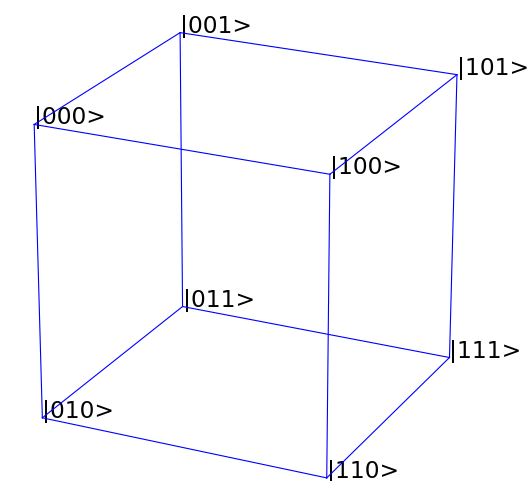
\includegraphics[width=0.35\textwidth]{img/cubewithoutprobs.png}
       \caption{\label{img:cubenoprobs} Visualising Hamming distances on a three-dimensional cube. The Hamming distance between two binary qubit patterns is given by the shortest path on the edges of the cube between them. Thereby, the Hamming distance increases by one for every corner.}
\end{figure}

\begin{minipage}[c]{.5\textwidth}
       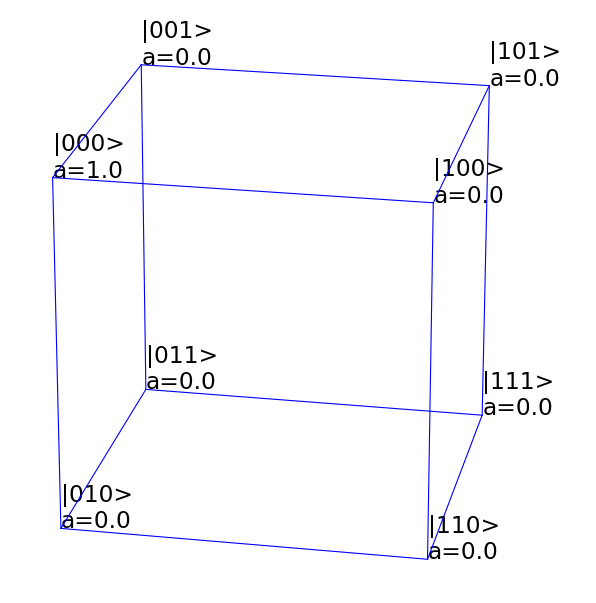
\includegraphics[width=1\textwidth]{img/cubeoneprob.png}
       \captionsetup{justification=raggedright, singlelinecheck=false}
       \captionof{figure}{\label{img:cubeoneprob} The qubit state $\ket{000}$ with amplitude ($a$) of 1.0 visualised on a three-dimensional cube representing the Hamming distances between binary qubit patterns.}
\end{minipage}%%%%%
%\begin{minipage}[c]{.5\textwidth}
%       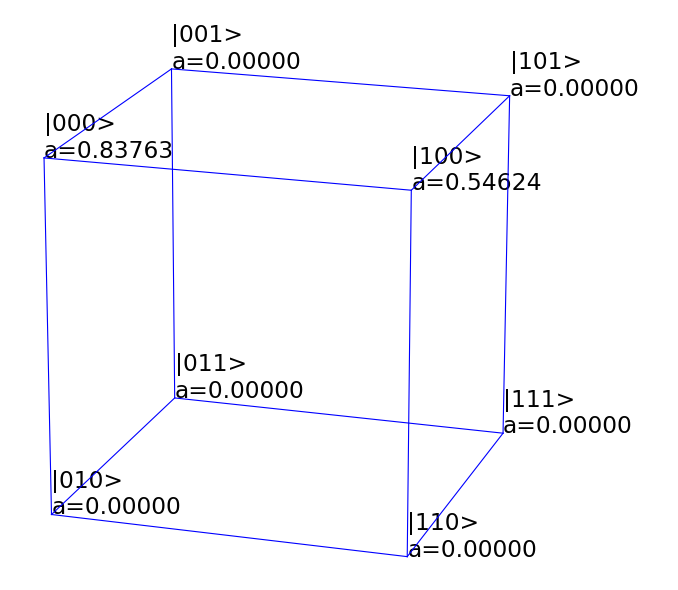
\includegraphics[width=1\textwidth]{img/cube_diffused1.png} \captionsetup{justification=raggedright, singlelinecheck=false}
%       \captionof{figure}{\label{img:cubediffused1} Visualisation of the amplitude distribution over all three-qubit states after application of coin gate $C$ to the first qubit of the state $\ket{000}$.}
%\end{minipage}
%\begin{minipage}[c]{.5\textwidth}
%       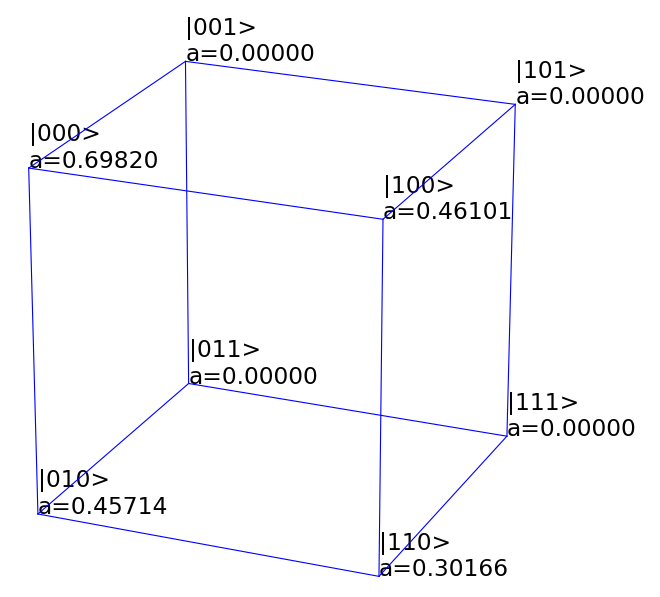
\includegraphics[width=1\textwidth]{img/cube_diffused2.png}
%       \captionsetup{justification=raggedright, singlelinecheck=false}
%       \captionof{figure}{\label{img:cubediffused2} Visualisation of the amplitude distribution over all three-qubit states after application of coin gate $C$ to the first two \\qubits in the state $\ket{000}$.}
%\end{minipage}%%%%%
\begin{minipage}[c]{.5\textwidth}
       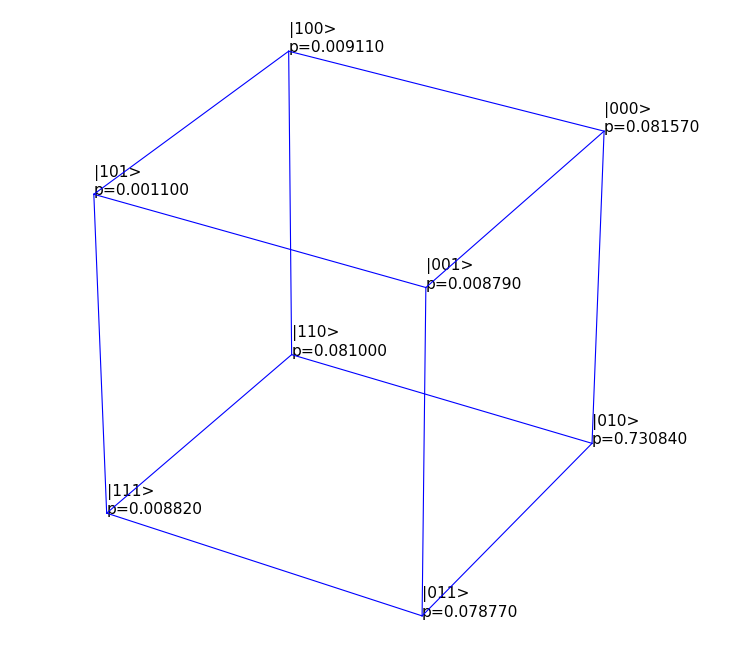
\includegraphics[width=1\textwidth]{img/cube_diffused.png} \captionsetup{justification=raggedright, singlelinecheck=false}
       \captionof{figure}{\label{img:cubediffused3} Final amplitude distribution over all three-qubit states after application of coin gate $C$ to each qubit in the state $\ket{000}$ visualised on a three-dimensional cube.}
\end{minipage}

The cube can now be used as another way of visualising the action of the coin gate $C(0.7)$ on each qubit in the $\ket{000}$ state. Before applying the $C$ gates the qubit state is $\ket{000}$ with an amplitude of 1.0 shown in Fig.~\ref{img:cubeoneprob} wherein amplitudes are denoted by $a$.
%Applying the coin gate $C$ to the first qubit redistributes the amplitudes between the $\ket{000}$ and $\ket{100}$ state which is visualised in Fig.~\ref{img:cubediffused1} below.
%Fig.~\ref{img:cubediffused2} illustrates the amplitude distribution after application of $C$ gates to the first and second qubit in the state $\ket{000}$. It can be seen that at this point already four out of eight three-qubit states have non-zero amplitudes.
After the application of the three $C(0.7)$ gates to the three qubits in $\ket{000}$ all eight-qubit patterns have non-zero amplitudes and the quantum state $\ket{w}$ from Eq.~\ref{equ:desiredmemorystate} is obtained. Fig.~\ref{img:cubediffused3} shows this final quantum superposition representing a discrete Gaussian distribution over a three-dimensional cube based on Hamming distances.
%In this example, Fig.~\ref{img:cubediffused1}, ~\ref{img:cubediffused2} and \ref{img:cubediffused3} visually demonstrated a stepwise diffusion of the initial amplitude 1.0 of $\ket{000}$ over all eight three-qubit patterns on the cube.

With the familiarisation with the coin gate $C$ and the use of cubes to visualise amplitude distributions, the introduction of most required tools to simulate the classification of Gaussian distributions with the aKNN algorithm is completed. Yet, since any distance-weighted kNN algorithm is based on measuring distances between the input sample and each training sample, a new distance metric for distributions needs to be introduced. For this reason, the Hellinger distance is defined in the red box below.

\begin{redbox}
\textbf{Definition: Hellinger distance}\\
\newline
The Hellinger distance is a distance metric used to quantify the difference between any two probability distributions. In the case of continuous probability distributions it is defined using the Hellinger integral first proposed by \citeA{hellinger1909neue}. However, since the $2^n$ amplitudes of an $n$-qubit system will always constitute a discrete probability distribution only the Hellinger distance for discrete distributions will be introduced.
\end{redbox}
\begin{redbox}
According to \citeA{harsha}, the Hellinger distance between two discrete probability distributions $R = (r_1,...,r_N)$ and $L = (l_1,...,l_N)$, each with $N$ entries, is defined as:

\begin{equation}
\label{equ:hellingerdistance}
H(R,L) = \frac{1}{\sqrt{2}}\sqrt{\sum_{i=1}^N (\sqrt{r_i} - \sqrt{l_i})^2}\, ,
\end{equation}
which can be rewritten in terms of the Euclidean distance between the square root vectors $\sqrt{R}$ and $\sqrt{L}$:
\begin{equation}
\label{equ:hellingereuclidean}
H(R,L) = \frac{1}{\sqrt{2}} \mid\mid\sqrt{R} - \sqrt{L}\mid\mid_2\, .
\end{equation}
Furthermore, the squared Hellinger distance can be expressed as
\begin{equation}
\label{equ:squaredhellingerdistance}
H^2(R,T) = \frac{1}{\sqrt{2}}\sum_{i=1}^N (\sqrt{r_i} - \sqrt{t_i})^2\, .
\end{equation}
\end{redbox}

Consequently, the aKNN algorithm should ideally classify Gaussian distributions based on their Hellinger distance and not based on Euclidean distance. Yet, Eq.~\ref{equ:hellingerdistance} and Eq.~\ref{equ:hellingereuclidean} revealed a strong relationship between the two distance metrics which can be exploited for the use in the aKNN algorithm. As previously discussed in Section~\ref{subsec:amplitudeKNNalgorithm}, the probability of measuring a certain class, e.g. $\ket{1}$, after the execution of the algorithm is given by
\begin{equation}
\label{equ:probcagain}
\mathrm{Prob}(\ket{c^m} = \ket{1})= \sum_{m \mid c^m=1} 1 - \frac{1}{4M} \sum_{i=1}^N \mid x_i - t^m_i \mid ^2\, .
\end{equation}

Suppose the probability distribution $R = (r_1,...,r_N)$ is the input sample that shall be classified and the distributions $L^m = (l_1^m,...,l_N^m)$ are the training samples. Instead of directly using them for the aKNN algorithm, one chooses their square root vectors such that $x_i \rightarrow \sqrt{r_i}$ and $t_i^m \rightarrow \sqrt{l_i^m}$. Eq.~\ref{equ:probcagain} then reads:
\begin{equation}
\mathrm{Prob}(\ket{c^m} = \ket{1})= \sum_{m \mid c^m=1} 1 - \frac{1}{4M} \sum_{i=1}^N \mid \sqrt{r_i} - \sqrt{l^m_i} \mid ^2\, ,
\end{equation}
which is now dependent on the squared Hellinger distance between the input distribution $R$ and each training distribution $L^m$.

It remains to discuss how to load the input and training distributions into the initial quantum state required for the amplitude-based kNN algorithm as defined in Eq.~\ref{equ:ampinitial}. The necessary procedure is outlined in Appendix~\ref{sec:stateprepgaussian}. Thus, all tools needed to classify Gaussian distributions with the amplitude-based kNN algorithm have been introduced.

The quantum simulation will be limited to discrete Gaussian distributions with eight entries, thus, making use of three data qubits with $2^3 = 8$ amplitudes. For the classification, two distinct Gaussian training distributions will be used. These training distributions should be chosen as different as possible to enable better classification results. The training dataset is listed in Table~\ref{tab:gausstrainingset}. The first training sample is selected to be a Gaussian distribution centred around $\ket{000}$ and is arbitrarily defined to be of class $\ket{0}$. The second training sample is defined to belong to class $\ket{1}$ and is chosen to be a Gaussian distribution centred around the $\ket{111}$ state. The cube in Fig.~\ref{img:cubenoprobs} illustrates that these are the most contrasting distributions because they are centred around diagonally opposite corners of the cube. Subsequently, the amplitude-based kNN algorithm will be evaluated on the input dataset listed in Table~\ref{tab:gaussinputset} which contains Gaussian distributions centred around the six binary three-qubit patterns that are not part of the training set.

\begin{minipage}[c]{.49\textwidth}
    \begin{tabular}{| C{0.8cm} | C{2.3cm} |C{2cm}|}
      \toprule
      ID & Gaussian distr. centered around & Class label\\
      \midrule
       1 & $\ket{000}$ & $\ket{0}$ \\\midrule
       2 & $\ket{111}$ & $\ket{1}$ \\
      \bottomrule
    \end{tabular}
        \label{tab:gausstrainingset}
        \captionsetup{justification=justified, singlelinecheck=false}
    \captionof{table}{Training dataset used for the classification of Gaussian distributions centered around different binary three-qubit patterns. The training dataset consists of two maximally different distributions with different class labels centered around diagonally opposite corners of the cube shown in Fig.~\ref{img:cubenoprobs}.}
\end{minipage}%%%%
\hspace{0.5cm}
\begin{minipage}[c][][b]{.49\textwidth}
\flushright
    \begin{tabular}{| C{0.8cm} | C{2.3cm} |C{2cm}|}
      \toprule
      ID & Gaussian distr. centered around & Expected class\\
      \midrule
       1 & $\ket{100}$ & $\ket{0}$ \\\midrule
       2 & $\ket{010}$ & $\ket{0}$ \\\midrule
       3 & $\ket{001}$ & $\ket{0}$ \\\midrule\midrule
       
       4 & $\ket{110}$ & $\ket{1}$ \\\midrule
       5 & $\ket{011}$ & $\ket{1}$ \\\midrule
       6 & $\ket{101}$ & $\ket{1}$ \\
      \bottomrule
    \end{tabular}
        \label{tab:gaussinputset}
        \captionsetup{justification=justified, singlelinecheck=false}
    \captionof{table}{Input dataset for the classification of Gaussian distributions with the amplitude-based kNN algorithm. The dataset contains Gaussian distributions centred around the six three-qubit patterns that are not part of the training dataset shown in Table~\ref{tab:gausstrainingset}. A particular input distribution is expected to be of the class for which the Hamming distance between the input distribution centre and the training distribution centre is smallest.}
\end{minipage}

The expected class label of an input distribution is dependent on the Hamming distance between its distribution centre and the distribution centre of the training samples. For example, looking at the cube in Fig.~\ref{img:cubenoprobs} reveals that the first input sample is a Gaussian distribution centred around $\ket{100}$ which is only one corner away from the distribution centre $\ket{000}$ of the first training sample. It is, however, two corners away from the distribution centre $\ket{111}$ of the second training sample. Thus, its expected class is that of the first training sample ($\ket{0}$).

Liqui$\ket{}$ was used to perform the quantum simulations, and the probability distributions for the classification of each input sample were collected within 1000 runs. The obtained simulation results are shown in Table~\ref{tab:gauss3qubitresults}. Note that all Gaussian distributions were initialised with the coin gate $C(\delta)$ whereby the shape of the resulting distribution depends on the parameter $\delta$ (as it was shown in Fig.~\ref{fig:gaussdeltaplot2}). It is, therefore, interesting to analyse how the value of $\delta$ alters the classification outcome. For this reason, three different values for $\delta$ were tested: In Table~\ref{tab:gauss3qubitresults} the results for $\delta = 0.6$ are always on top and marked with an empty circle ($\circ$), results for $\delta = 0.85$ are always in the middle marked with a filled circle ($\bullet$) and results for $\delta = 0.95$ are always at the bottom and marked with a triangle ($\triangleright$).

\begin{table}[H]
\begin{tabular}{| C{0.5cm} | C{2.7cm} |C{1.7cm} | C{1.7cm} | C{1.7cm} |C{1.8cm}| C{1.8cm}|}
      \toprule
      ID & Gaussian distr. centered around & $\mathrm{Prob(CM)}$ & $\mathrm{Prob}$ $(\ket{c} = \ket{0})$ & $\mathrm{Prob}$ $(\ket{c} = \ket{1})$ & Expected class & Algorithm output\\
      \midrule
        1 & $\ket{100}$ & \begin{tabular}{c} 0.9930$^\circ$ \\\midrule 0.8090$^\bullet$ \\\midrule 0.6740$^\triangleright$ \end{tabular} & \begin{tabular}{c} 0.4904$^\circ$ \\\midrule 0.5414$^\bullet$ \\\midrule 0.5549$^\triangleright$ \end{tabular} & \begin{tabular}{c} 0.5096$^\circ$ \\\midrule 0.4586$^\bullet$ \\\midrule 0.4451$^\triangleright$ \end{tabular} & $\ket{0}$ & \begin{tabular}{c} $\ket{1}$ $^\circ$ \\\midrule $\ket{0}$ $^\bullet$ \\\midrule $\ket{0}$ $^\triangleright$ \end{tabular}\\\midrule
        
       2 & $\ket{010}$ & \begin{tabular}{c} 0.9830$^\circ$ \\\midrule 0.8050$^\bullet$ \\\midrule 0.6600$^\triangleright$ \end{tabular} & \begin{tabular}{c} 0.4914$^\circ$ \\\midrule 0.5205$^\bullet$ \\\midrule 0.5636$^\triangleright$ \end{tabular} & \begin{tabular}{c} 0.5086$^\circ$ \\\midrule 0.4795$^\bullet$ \\\midrule 0.4364$^\triangleright$ \end{tabular}& $\ket{0}$ & \begin{tabular}{c} $\ket{1}$ $^\circ$ \\\midrule $\ket{0}$ $^\bullet$ \\\midrule $\ket{0}$ $^\triangleright$ \end{tabular}\\\midrule
       
       3 & $\ket{001}$ & \begin{tabular}{c} 0.8280$^\circ$ \\\midrule 0.8120$^\bullet$ \\\midrule 0.6700$^\triangleright$ \end{tabular} & \begin{tabular}{c} 0.4980$^\circ$ \\\midrule 0.5582$^\bullet$ \\\midrule 0.5642$^\triangleright$ \end{tabular} & \begin{tabular}{c} 0.5020$^\circ$ \\\midrule 0.4418$^\bullet$ \\\midrule 0.4358$^\triangleright$ \end{tabular} & $\ket{0}$ & \begin{tabular}{c} $\ket{1}$ $^\circ$ \\\midrule $\ket{0}$ $^\bullet$ \\\midrule $\ket{0}$ $^\triangleright$ \end{tabular}\\\midrule\midrule
       
       4 & $\ket{110}$ & \begin{tabular}{c} 0.9830$^\circ$ \\\midrule 0.8040$^\bullet$ \\\midrule 0.6350$^\triangleright$ \end{tabular} & \begin{tabular}{c} 0.4914$^\circ$ \\\midrule 0.4726$^\bullet$ \\\midrule 0.4520$^\triangleright$ \end{tabular} & \begin{tabular}{c} 0.5086$^\circ$ \\\midrule 0.5274$^\bullet$ \\\midrule 0.5480$^\triangleright$ \end{tabular} & $\ket{1}$ &\begin{tabular}{c} $\ket{1}$ $^\circ$ \\\midrule $\ket{1}$ $^\bullet$ \\\midrule $\ket{1}$ $^\triangleright$ \end{tabular} \\\midrule
        
       5 & $\ket{011}$ & \begin{tabular}{c} 0.9830$^\circ$ \\\midrule 0.8300$^\bullet$ \\\midrule 0.6730$^\triangleright$ \end{tabular} & \begin{tabular}{c} 0.4964$^\circ$ \\\midrule 0.4398$^\bullet$ \\\midrule 0.4383$^\triangleright$ \end{tabular} & \begin{tabular}{c} 0.5036$^\circ$ \\\midrule 0.5602$^\bullet$ \\\midrule 0.5617$^\triangleright$ \end{tabular}& $\ket{1}$ & \begin{tabular}{c} $\ket{1}$ $^\circ$ \\\midrule $\ket{1}$ $^\bullet$ \\\midrule $\ket{1}$ $^\triangleright$ \end{tabular}\\\midrule
       
       6 & $\ket{101}$ & \begin{tabular}{c} 0.9840$^\circ$ \\\midrule 0.8110$^\bullet$ \\\midrule 0.6320$^\triangleright$ \end{tabular} & \begin{tabular}{c} 0.4888$^\circ$ \\\midrule 0.4451$^\bullet$ \\\midrule 0.4320$^\triangleright$ \end{tabular} & \begin{tabular}{c} 0.5112$^\circ$ \\\midrule 0.5549$^\bullet$ \\\midrule 0.5680$^\triangleright$ \end{tabular} & $\ket{1}$ & \begin{tabular}{c} $\ket{1}$ $^\circ$ \\\midrule $\ket{1}$ $^\bullet$ \\\midrule $\ket{1}$ $^\triangleright$ \end{tabular}\\
       
      \bottomrule
    \end{tabular}
    \caption{\label{tab:gauss3qubitresults} Amplitude-based kNN algorithm classification results after 1000 runs for various Gaussian distributions centered around six different three-qubit patterns. The Gaussian distributions were created using the coin gate $C(\delta)$. For each pattern three different distributions were prepared and classified by changing the parameter $\delta$: The results for $\delta = 0.6$ are always on top and marked with an empty circle ($\circ$), results for $\delta = 0.85$ are always in the middle marked with a filled circle ($\bullet$) and results for $\delta = 0.95$ are always at the bottom and marked with a triangle ($\triangleright$)}
\end{table}

The results in Table~\ref{tab:gauss3qubitresults} show that for all input distributions the probability of a successful conditional measurement $\mathrm{Prob}(\mathrm{CM})$ decreases with increasing values of $\delta$. Specifically, in the case $\delta = 0.6$ the values of $\mathrm{Prob}(\mathrm{CM})$ are very close to unity for all six input distributions. Furthermore, when $\delta = 0.6$ the probability distributions over the class qubit states \0 and \1 are close to being equal for all six input distributions indicating no clear preference for a particular class. This can be explained by looking back to Fig.~\ref{fig:gaussdeltaplot2} which shows that choosing $\delta = 0.6$ results in flat Gaussian distributions with little peaks. On the cube in Fig.~\ref{img:cubenoprobs} this would correspond to an almost uniform amplitude distribution over the cube. In this case, the training samples are almost equal to each other yielding nearly equal probabilities for class \0 and \1 for all six input distributions. As a result, for $\delta = 0.6$ the first three input distributions were all incorrectly classified, and the last three input samples were all correctly classified. Despite correct or incorrect classification, all six class qubit probability distributions show no clear preference and make clear that the training samples with $\delta = 0.6$ are not distinct enough for the algorithm to make a clear classification decision.

In the case $\delta = 0.85$ all six input distributions were correctly classified. In this case, the Gaussian training distributions correspond to more distinct amplitude distributions over the cube in Fig.~\ref{img:cubenoprobs}. This fact results in different probabilities for class \0 and \1, thereby clearly favouring one class over the other. Lastly, for $\delta = 0.95$ all six input distributions were again correctly classified with larger differences between the probabilities for class \0 and \1 compared to the case $\delta = 0.85$.


%Summarize the Gaussian part
%Stress that it was another toy example for the aKNN algorithm
%Need to implement more advanced state preparation algorithms!
%aKNN performed well for the fact that it is a very simple q alg



%Summarize the entire Results & Discussion section here?
%Contrast with some other work if possible
%Criticize what could be improved




%This way of visualising HDs can be extended to the 16 binary patterns made by four qubits that can be visualised on a 4-D cube, also called tesseract, as illustrated in Fig.~\ref{img:hypercubenoprobs}.

%\begin{figure}[!ht]
%       \centering
%       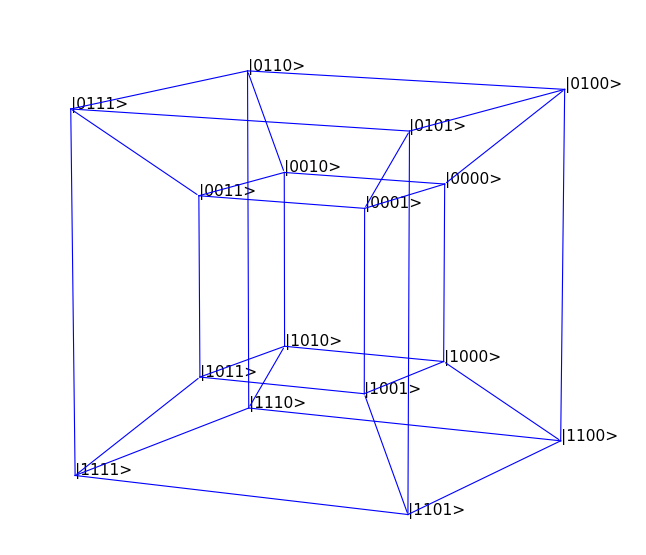
\includegraphics[width=0.5\textwidth]{img/hypercubewithoutprobs.png}
%       \caption{\label{img:hypercubenoprobs} Visualizing Hamming distances on a 4-D cube (tesseract)}
%\end{figure}

%Initialising gaussian distributed quantum states and classifying gaussian distributions by means of the Hellinger distance.
\chapter{Outlook}\label{sec:outlook}

Despite the use of small classification problems, neither the qubit- nor the amplitude-based kNN algorithm could be implemented on the quantum hardware provided by the IBM Quantum Experience (IBMQE). Thereby, the limiting factors were the small number of qubits as well as the small universal gate set consisting of only ten quantum gates. Yet, the latter issue might soon be resolved since IBM has made an announcement in the IBMQE discussion forum that there will be a major update to IBMQE 2.0 soon. According to IBM researcher \citeA{ibmquasm2.0}, this update will provide a larger universal gate set including more general rotation gates. However, it is unclear at this point if IBM will enable the use of more than 40 gates in their quantum composer. The author of this thesis will retry an implementation of the amplitude-based kNN algorithm as soon as this update has been rolled out. Future research might also consider the implementation of other quantum machine learning algorithms with small datasets using the IBMQE 2.0.

For this research relatively simple quantum state preparation routines were used. This was deliberately chosen since the timeframe of this thesis did not allow for the implementation of more sophisticated quantum state preparation algorithms. Future research should, therefore, focus on simulation and actual implementation of quantum algorithms initialising arbitrary amplitude distributions. This might provide insights into which types of classical data can be encoded into amplitudes as well as what resources are needed to do so.

Lastly, this bachelor thesis research was presented at the 4\textsuperscript{th} South African Conference for Quantum Information Processing, Communication and Control in Cape Town which sparked the interest of an experimental research group working on quantum computation based on trapped ions in Israel. Furthermore, there is the possibility for a collaboration with an experimental group working on nuclear magnetic resonance quantum computation in China. Shortly, one of the possible collaborations could lead to an experimental implementation and subsequent publication of the amplitude-based kNN algorithm by \citeA{SchuldFingerhuth}.

%Experimental implementation with an experimental quantum computation group
%possibly NMR, photonic or trapped ions

\chapter{Personal Reflection}\label{sec:personalreflection}

This bachelor thesis research has been instructive and beneficial in many different ways. Most importantly, I have had the opportunity to dedicate my entire time to learn about the subject of quantum information and, specifically, quantum machine learning in detail. Since these subjects are not taught within the curriculum of the Maastricht Science Programme (MSP) it was especially amazing to challenge myself with these notoriously difficult subjects within the intersection of quantum physics and computer science. In doing so, I have learned more about the methods of theoretical physics and gained additional experience in scientific programming with Octave, Python and F\#. Without prior knowledge of F\#, I was able to learn how to simulate quantum computations and quantum machine learning algorithms using the quantum simulation toolsuite Liqui$\ket{}$. Furthermore, I was able to use the first cloud-based quantum computer, the so-called IBM Quantum Experience, publicly released in May 2016 by IBM.

Alongside my research, I had the possibility to attend many great lectures, seminars and three conferences which were all generously funded by the Centre for Quantum Technology. This enabled me to get to know many renowned scientists working in the fields of quantum information, quantum machine learning, open quantum systems, quantum optics and quantum cryptography. Furthermore, I was provided with the opportunity to present my research at the 4\textsuperscript{th} South African Conference for Quantum Information Processing, Communication and Control in Cape Town in late November 2016. This constituted a big step with respect to my academic career and a great way of putting my acquired presentation skills to practice.

However, in retrospect I feel that I could have been more productive in office by structuring my work days more diligently. For example, the first one and a half months were mostly spent on reading research paper and text books to acquire the theoretical foundation for my research and little time was used to practice F\# within the Liqui$\ket{}$ framework. A possible solution for the future would be to divide each day into two parts: e.g. spending the morning with reading papers and books and the afternoon on practical work and programming. Besides this, I feel like I should have communicated my progress more with my internal supervisor Dr. Birembaut at the MSP.

In conclusion, the bachelor thesis research has showed me the importance of interdisciplinarity since the field of quantum information requires the understanding of concepts in computer science as well as quantum mechanics. Fortunately, MSP's liberal education does not only focus on textbook exercises and lectures but mostly teaches us how to systematically approach unknown topics and tackle problems therein. It was great to see that this enabled me to venture into a previously unfamiliar field and learn the necessary skills to conduct meaningful research. The newly acquired skills will certainly be useful for my planned masters in the field of quantum information.

%During the thesis work, I realized that encountering problem after problem is at the core of research but that one can resolve most of them when just showing enough dedication.

%The Centre for Quantum Technology at the University of KwaZulu-Natal in South Africa has been a wonderful host for my Bachelor thesis research. My supervisor Prof. Francesco Petruccione has become a mentor and friend and provided me with great opportunities for personal and academic growth. Furthermore, my collaborator Maria Schuld has shared vasts amount of knowledge, tricks and ideas with me and has always been a great help during my research work. Alongside my research, I had the possibility to attend many great lectures, seminars and three conferences which were all generously funded by the Centre for Quantum Technology. This enabled me to get to know many renowned scientists working in the fields of quantum information, quantum machine learning, open quantum systems, quantum optics and quantum cryptography. Attending the Quantum Machine Learning Workshop at the Dolphin Coast in July 2016 provided me with a broad overview of the field of quantum machine learning and was the first time that I ever attended a scientific conference. In November 2016, I was provided with the opportunity to present my research at the 4\textsuperscript{th} South African conference for Quantum Information Processing, Communication and Control in Cape Town. This opened the possibility for a collaboration with an experimental research group in Israel working on quantum computation with trapped ions. In January 2017, I am invited to the NiTheP Chris Engelbrecht Quantum Machine Learning Summer School where I will give three workshop sessions on quantum machine learning using the Liqui$\ket{}$ framework and the IBM Quantum Experience.

\chapter{Quantum state preparation routine for Gaussian distributions}\label{sec:stateprepgaussian}

To keep the discussion simple, the task is to load one Gaussian input distribution $R$ and two Gaussian training samples; $L_1$ and $L_2$, such that the amplitude-based kNN algorithm can be used to classify $R$. Note that the input and training distributions are restricted to Gaussian distributions that can be initialized by using the coin gate $C(\delta)$ for some value of $\delta$. The input and training samples all have $N$ entries whereby $N$ is restricted to be a multiple of two. To encode the distributions, $n$ data qubits are required such that there are $2^n = N$ amplitudes. Additionally, one ancilla, one class and one $m$ qubit are needed. Since all qubits are initialised to the \0 state, the initial state is 

\begin{equation}
\ket{\Upsilon_0} = \ket{a;d_1,...,d_n;c;m} = \ket{0;0_1,...,0_n;0;0}
\end{equation}

where the first register holds the ancilla ($a$), the second register contains the $n$ data qubits ($d$) used to encode the distributions and the third and fourth register consists of the class ($c$) and $m$-qubit respectively.

As already demonstrated in Eq.~\ref{equ:chi1} and Eq.~\ref{equ:chi2} in Section~\ref{subsubsec:implementationamplitudeKNN}, the ancilla and $m$-register are each put into an equal superposition through the application of two H gates. The state is then

\begin{equation}
\ket{\Upsilon_1} = \frac{1}{2} \sum_{m=0}^1 \big[ \ket{0}\ket{0_1,...,0_n} + \ket{1}\ket{0_1,...,0_n}\big] \ket{0}\ket{m}
\end{equation}

Suppose the Gaussian distribution $R$ is obtained by choosing $\delta = \tau$ for the coin gate $C(\delta)$. Then the next step is to make use of the controlled version of the coin gate $CC(\tau)$ controlled by the ancilla qubit. $CC(\tau)$ is applied to each of the $n$ qubits in the data register to load the input distribution $R$. Hence, the new quantum state is 

\begin{equation}
\ket{\Upsilon_2} = \prod^n_{j=1} CC(\tau)(a,d_j) \ket{\Upsilon_1} = \frac{1}{2} \sum_{m=0}^1 \big[ \ket{0}\ket{0_1,...,0_n} + \ket{1}\ket{R}\big] \ket{0}\ket{m}
\end{equation}

Since the algorithm is simulated in Liqui$\ket{}$, it is straightforward to define the controlled version of the coin gate $C(\delta)$. 

Next, using an X gate to flip the ancilla moves the input distribution $R$ onto the \0 state of the ancilla such that the state is now

\begin{equation}
\ket{\Upsilon_3} = X(a) \ket{\Upsilon_2} = \frac{1}{2} \sum_{m=0}^1 \big[ \ket{0}\ket{R} + \ket{1}\ket{0_1,...,0_n}\big] \ket{0}\ket{m}
\end{equation}

Suppose the first training distribution $L_1$ can be loaded by choosing $\delta = \sigma$ and applying $C(\sigma)$ to the qubit pattern $\ket{0_1,...,1_5,0_6,...,0_n}$. Thus, the fifth qubit in the data register connected to the \1 ancilla state needs to flipped into the \1 state. This can be done with a CCNOT gate, controlled by the ancilla and $m$ qubit, acting on the fifth data qubit. Next, by applying the controlled controlled version of the coin gate $CCC(\sigma)$ to each data qubit controlled by the ancilla and the $m$ qubit the training sample $L_1$ is loaded. The quantum state is then given by
\begin{align}
\ket{\Upsilon_4} &= \prod^n_{j=1} CCC(\sigma)(a,m,d_j) CCNOT(a,m,d_5) \ket{\Upsilon_3}\notag\\
&= \frac{1}{2} \Big[\big[ \ket{0}\ket{R} + \ket{1}\ket{0_1,...,0_n}\big] \ket{0}\ket{0} + \big[\ket{0}\ket{R} + \ket{1}\ket{L_1*}\big] \ket{0}\ket{1}\Big]
\end{align}

Since the last entry on the diagonal of the coin gate (see Eq.~\ref{equ:coingate}) is negative, the application of $CCC(\sigma)$ introduces a negative sign when applied to the fifth data qubit. Hence, not the exact distribution $L_1$ but a distribution $L_1^*$ with a sign difference was loaded into $\ket{\Upsilon_4}$. As explained in Section~\ref{subsec:amplitudeKNNalgorithm}, the amplitude-based kNN algorithm makes use of interference between the input and training samples whereby the negative sign would alter the outcome of the interference. Thus, the sign needs to be corrected by acting a controlled controlled Z gate on the fifth data qubit. Thereafter, the $m$ qubit is flipped with an X gate to move $L_1$ onto the \0 state of the $m$ qubit. After these gate operations the state is
\begin{align}
\ket{\Upsilon_5} &= X(m) CCZ(d_5) \ket{\Upsilon_4}\notag\\
&= \frac{1}{2} \Big[\big[ \ket{0}\ket{R} + \ket{1}\ket{L_1}\big] \ket{0}\ket{0} + \big[\ket{0}\ket{R} + \ket{1}\ket{0_1,...,0_n}\big] \ket{0}\ket{1}\Big]
\end{align}

For the second training distribution $L_2$, suppose it results from choosing $\delta = \nu$ and applying $C(\nu)$ to the qubit pattern $\ket{1_1,...,1_n}$. Thus, all data qubits connected to the \1 ancilla and \1 $m$-qubit state have to be flipped using a CCNOT gates. As outlined in the previous step, $CCC(\nu)$ loads the distribution $L_2^*$ and not $L_2$ because of sign differences. Since all data qubits are \1, these signs are corrected by acting controlled controlled Z gates on all data qubits controlled by the ancilla and $m$-qubit. The state containing the input and both training distributions is then

\begin{align}
\ket{\Upsilon_6} &= \prod^n_{j=1} CCZ(d_j) CCC(\sigma)(a,m,d_j) CCNOT(a,m,d_j) \ket{\Upsilon_5}\notag\\
&= \frac{1}{2} \Big[\big[ \ket{0}\ket{R} + \ket{1}\ket{L_1}\big] \ket{0}\ket{0} + \big[\ket{0}\ket{R} + \ket{1}\ket{L_2}\big] \ket{0}\ket{1}\Big]
\end{align}

Lastly, the class qubit for $L_2$ is flipped with a CNOT gate controlled by the $m$ qubit such that the final state is
\begin{align}
\ket{\Upsilon_6} &= CNOT(m,c) \ket{\Upsilon_6}\notag\\
&= \frac{1}{2} \Big[\big[ \ket{0}\ket{R} + \ket{1}\ket{L_1}\big] \ket{0}\ket{0} + \big[\ket{0}\ket{R} + \ket{1}\ket{L_2}\big] \ket{1}\ket{1}\Big]
\end{align}


$\ket{\Upsilon_7}$ is in the form of the initial quantum state (Eq.~\ref{equ:ampinitial}) required for the amplitude-based kNN algorithm. This completes the quantum state preparation routine for loading a restricted subset of discrete Gaussian distributions using the coin gate $C(\delta)$.

 \cleardoublepage
